%-*- coding: utf-8 -*-
\documentclass[11pt,a4paper,twoside,openright]{book} %report
%-*- coding: utf-8 -*-
\usepackage[utf8]{inputenc}
%\usepackage[T1]{fontenc}
\usepackage{lmodern}
\usepackage[francais]{babel}
\usepackage[babel=true]{csquotes} % csquotes va utiliser la langue définie dans babel
\usepackage{hyperref}
	\hypersetup{colorlinks,%
	citecolor=black,%
	filecolor=black,%
	linkcolor=black,%
	urlcolor=blue}
\usepackage{graphicx}
	\graphicspath{{images/}}
\usepackage[left=2.0cm,right=2.0cm,top=2.0cm,bottom=2.0cm]{geometry}

\usepackage[table, dvipsnames]{xcolor}

\usepackage{tocvsec2}
\maxsecnumdepth{all}
\usepackage{glossaries}
\makeglossaries

% Pour supprimer le mot 'Chapitre'
\usepackage{titlesec}
\titleformat{\chapter}[hang]{\bf\huge}{\thechapter}{2pc}{}

% Pour les entêtes et pieds de pages
\usepackage{fancyhdr}

%%%%%%%%%%%%%%%%%%%style front%%%%%%%%%%%%%%%%%%%%%%%%%%%%%%%%%%%%%%%%%
	\fancypagestyle{front}{%
  		\fancyhf{}%on vide les entêtes
  		\fancyfoot[C]{page \thepage}%
  		\renewcommand{\headrulewidth}{0pt}%trait horizontal pour l'entête
  		\renewcommand{\footrulewidth}{0.4pt}%trait horizontal pour les pieds de pages
		}

%%%%%%%%%%%%%%%%%%%style main%%%%%%%%%%%%%%%%%%%%%%%%%%%%%%%%%%%%
	\fancypagestyle{main}{%
		\fancyhf{}
		\fancyhead[c]{\textbf{VITAMEAL -}}
		\fancyfoot[C]{Formation Ingénieur Informatique en alternance - Première année}
		\fancyfoot[RO,LE]{\textbf{CNAM}}%
  		\fancyfoot[LO,RE]{\textbf{\thepage/\pageref{LastPage}}}
  		\renewcommand{\headrulewidth}{0.4pt}%trait horizontal pour l'entête
  		\renewcommand{\footrulewidth}{0.4pt}%trait horizontal pour les pieds de pages
  		}

%%%%%%%%%%%%%%%%%%%style plain%%%%%%%%%%%%%%%%%%%%%%%%%%%%%%%%%%%%
	\fancypagestyle{plain}{%
		\fancyhf{}
		\fancyhead[c]{\textbf{VITAMEAL -}}
		\fancyfoot[C]{Formation Ingénieur Informatique en alternance - Première année}
		\fancyfoot[RO,LE]{\textbf{CNAM}}%
  		\fancyfoot[LO,RE]{\textbf{\thepage/\pageref{LastPage}}}
  		\renewcommand{\headrulewidth}{0.4pt}%trait horizontal pour l'entête
  		\renewcommand{\footrulewidth}{0.4pt}%trait horizontal pour les pieds de pages
  		}

%%%%%%%%%%%%%%%%%%%style back%%%%%%%%%%%%%%%%%%%%%%%%%%%%%%%%%%%%%%%%%
	\fancypagestyle{back}{%
  		\fancyhf{}%on vide les entêtes
  		\fancyfoot[C]{page \thepage}%
  		\renewcommand{\headrulewidth}{0pt}%trait horizontal pour l'entête
  		\renewcommand{\footrulewidth}{0.4pt}%trait horizontal pour les pieds de pages
		}

\usepackage{float}
%\frenchbsetup{StandardLists=true}
\usepackage{pifont}
\usepackage{enumitem}
\setlistdepth{9}
\setlist[itemize,2]{label=$\triangleright$}
\setlist[itemize,3]{label=$\bullet$}
\setlist[itemize,4]{label=\ding{226}}
\renewlist{itemize}{itemize}{9}

\usepackage{wasysym}
\usepackage{amssymb}
\usepackage[section]{placeins}


\begin{document}
\let\cleardoublepage\clearpage
\frontmatter
\pagestyle{front}
%-*- coding: utf-8 -*-
%\phantomsection
\begin{titlepage}
\color[RGB]{91, 155, 213}
\parindent=0pt

\begin{center}

\includegraphics[scale=1.0]{images/deco1.png}%
\end{center}

\hrulefill
\begin{center}\bfseries\Huge
    PROJET VITAMEAL
\end{center}
\hrulefill

\begin{center}\bfseries\Large
Restauration hospitalière
\end{center}

\begin{center}

\includegraphics[scale=1.0]{images/deco2.png}%
\end{center}

\vspace*{1cm}
\begin{center}\bfseries\Large
Nicolas SYMPHORIEN

Sonia OTHMANI

Jean-Félix BENITEZ
\end{center}

\vspace*{\stretch{2}}

CNAM \hspace*{\stretch{1}} Formation en alternace

Ingénieur Informatique \hspace*{\stretch{1}} Première année

\end{titlepage}

\thispagestyle{empty}                        % pour la page de garde toute blanche

\mainmatter
\pagestyle{main}
%-*- coding: utf-8 -*-
\begin{center}\bfseries\Huge
    Feuille de suivi des évolutions
\end{center}
\begin{tabular}{|c|p{3.5cm}|c|p{9cm}|}
  \hline
  Indice & Éléments concernés & Date & Raison et nature de l'évolution \\ \hline
  - & Toutes les pages & 09/03/2017 & Création du document\\
  - & Élaboration & 11/03/2017 & Ajout de la description de l'usine logicielle\\
  - & Initialisation & 28/03/2017 & Ajout du document sur la nutrition en référence, avec ses exigences liées.\\
  - & Initialisation & 29/03/2017 & Ajout du contexte du problème.\\
  - & Initialisation & 29/03/2017 & Ajout d'un schema de modélisation du problème\\
  - & Initialisation & 30/03/2017 & 2 petits ajustements.\\
  - & Exigences & 30/03/2017 & Correction des incohérences dans les exigences.\\
  - & Les besoins & 13/04/2017 & Enrichissement des besoins.\\
  - & Annexe A & 13/04/2017 & Ajout d'une annexe sur la composition des petits-déjeuner\\
  - & Annexe A & 15/04/2017 & Ajout de la partie déjener sur l'annexe A\\
  - & Les besoins & 16/04/2017 & Corrections, reformulations de certains besoins.\\
  - & Annexe A & 20/04/2017 & Replacement partie composition des repas par une annexe\\
  - & Exigences & 22/04/2017 & Ajout des exigences extrètes du référentiel.\\
  - & Exigences & 22/04/2017 & Mise à jour des exigences.\\
  - & Périmètre & 23/04/2017 & Exclusion des personnes agées du périmètre du projet.\\
  - & Les besoins & 24/04/2017 & Mise à jour des besoins.\\
  - & Exigences & 24/04/2017 & Ajout d'exigences.\\
  - & Exigences & 29/04/2017 & Passage \No exigences sur 5 digit.\\
  - & Exigences & 29/04/2017 & Numérotation des besoins, mise à jour des exigences.\\
  - & Ajout Exigences & 29/04/2017 & Ajout d'un champ nature dans les exigences.\\
  - & Cas d'utilisations & 06/05/2017 & Ajout de la génération automatique des menus.\\
  - & Cas d'utilisations & 07/05/2017 & Correction cas d'utilisation et rapport.\\
  - & Cas d'utilisations & 08/05/2017 & Intégration des use case dans le rapport\\
  - & Exigences & 08/05/2017 & Correction exigences.\\
  - & Backlog & 08/05/2017 & Mise en place du Backlog.\\
  - & Backlog & 09/05/2017 & Enrichissement du backlog.\\
  - & Cas d'utilisation  & 10/05/2017 & Ajout d'un cas d'utilisation.\\
  - & Élaboration  & 11/05/2017 & Mise à jour usine logiciel dans le rapport\\
  - & Cas d'utilisation & 12/05/2017 & Remplacement de générer par élaborer les menus.\\
  - & & 12/05/2017 & Suppression des chapitres restant à faire qui n'ont plus de sens.\\
  - & Cas d'utilisation & 15/06/2017 & Enrichissement de l'élaboration des menus et ajout du diagramme de séquences. Ajout du modèle de domaine.\\
  - & Cas d'utilisation & 17/06/2017 & Ajout du modèle conceptuel de données. \\
  - & Cas d'utilisation & 28/06/2017 & Génération des menus: ajout du diagramme de séquences détaillé, du diagramme des classes et de la description de l'algorithme.\\
  - & Cas d'utilisation & 03/07/2017 & Composition d'un plat: ajout du diagramme de séquences détaillé, du diagramme des classes et des maquettes.\\
  &&&\\
  &&&\\
  &&&\\
  &&&\\
  &&&\\
  &&&\\ \hline
\end{tabular}

\tableofcontents
\listoffigures
\listoftables
%-*- coding: utf-8 -*-
\textcolor[RGB]{46, 116, 181}{\chapter{Présentation}}
\section{Objet du document}
Ce document est le rapport du travail fait sur le projet d'outil informatique destiné à la restauration hospitalière.

\section{Domaine d'application}
Formation du CNAM en ingénieur informatique première année.

\section{Description du document}
Les trois premiers chapitres définissent le contenu de ce document~; les chapitres suivants décrivent le travail fait sur ce projet.

\section{Emplacement du document}
\href{https://github.com/Seikomi/Vitameal/tree/master/doc}{\emph{https://github.com/Seikomi/Vitameal/tree/master/doc}}


%-*- coding: utf-8 -*-
\textcolor[RGB]{46, 116, 181}{\chapter{Documents}}
\section{documents applicables}
Sans objet.
\section{documents de référence}
\setenumerate{font=\bfseries, label=R\arabic*}
\begin{enumerate}
\item\label{docNutrition} RECOMMANDATION NUTRITION, Version 2.0 – JUILLET 2015, (nutrition.pdf)

\url{http://www.economie.gouv.fr/daj/recommandation-nutrition}
\end{enumerate}

%-*- coding: utf-8 -*-
\textcolor[RGB]{46, 116, 181}{\chapter{Terminologie}}
\section{Abréviations}
\rowcolors{1}{red!26!green!29!blue!31!}{}
\begin{table}[!h]
\begin{tabular}{p{2.5cm}p{13.5cm}}
  &\\
  &\\
  &\\
  &\\
  &\\
  &\\
  &\\
\end{tabular}
\caption{abréviations}
\end{table}

\section{Glossaire}
\begin{table}[!h]
\begin{tabular}{lp{13.5cm}}
  \textbf{Ingrédients} & Aliments de bases \\
  \textbf{Produits} & Composé de plusieurs aliments \\
  &\\
  &\\
  &\\
  &\\
  &\\
\end{tabular}
\caption{glossaire}
\end{table}
\printglossaries

%-*- coding: utf-8 -*-
\textcolor[RGB]{46, 116, 181}{\chapter{Contexte et problème}}
Quelle que soit l’importance des avancées scientifiques et technologiques, c’est le travail des
professionnels de santé qui détermine la qualité et l’efficacité des soins. Dans ce contexte, les soins
nutritionnels, qui portent sur l’évaluation de l’état nutritionnel et l’accompagnement alimentaire des
patients hospitalisés, en interaction étroite avec l’équipe de soin, ne font pas exception. Pour ce
faire, les diététiciens développent des actions de complexité variable, tant au niveau des services de
soins que du système de restauration.

Simultanément, les professionnels doivent faire face à de nouveaux défis, dus aux modifications des
profils épidémiologiques, démographiques et sociaux des populations, ce qui exige la mise en place
de nouvelles compétences et la reconfiguration des stratégies d’action. Pour les diététiciens du
secteur hospitalier, elles ont pour conséquences de nouvelles exigences mentales et surtout
cognitives.

Le niveau de développement industriel de la filière alimentaire française allège la charge de travail
technique des diététiciens, non seulement en ce qui concerne la diversité de matières premières,
mais également dans le domaine du contrôle \enquote{qualité}, tout au long de la chaîne de production. De
la même façon, les nouveaux concepts de production en restauration collective, caractérisés par
l’utilisation de produits pré élaborés et l’innovation technologique des équipements, gagnent
visiblement du terrain dans le secteur hospitalier français.

\section{Définition du problème}
L'élaboration de menus dans un hôpital pour la restauration des patients
est une tâche complexe, et doit tenir compte des différentes pathologies
rencontrées. Faute de moyens (temps et argent) seules quelques grandes
lignes de restauration sont retenues; alors qu'idéalement, chaque
patient devrait pourvoir avoir un repas adapté à sa pathologie.

\section{Vision du projet}
\subsection{Solution envisagée}
Le projet Vitameal a pour objectif de faire correspondre au mieux la planification des régimes et des
prescriptions diététiques aux repas réellement servis au patient. Il consiste en un outil interfaçant la
gestion de production, la prise de commande et le suivi nutritionnel des repas.

\subsection{Périmètre}
C'est un diététicien qui renseigne le profil diététique des patients,
sous les directives des médecins. C'est aussi un diététicien qui élabore
les menus des patients. L'outil élaborera donc
les menus par filtrage des produits correspondants aux profils
diététiques des patients. Pour des raisons de simplifications, nous nous limiterons dans ce projet aux seuls patients adolescents et adultes, à l'exclusion des personnes agées.
\begin{figure}[H]
\label{Modelisation_du _probleme}
  \centering
      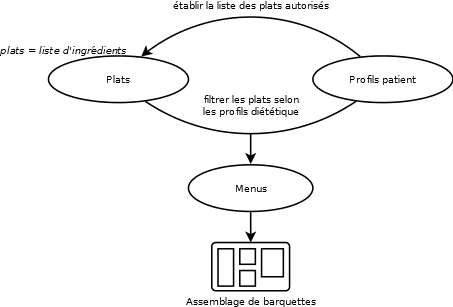
\includegraphics[width=0.75\textwidth]{problem_model} %
\caption{Modélisation du problème}
\end{figure}


%-*- coding: utf-8 -*-
\textcolor[RGB]{46, 116, 181}{\chapter{Méthode de travail}}
\section{Organisation}
\subsection{Planification des activités}
Nous fixons la date de livraison à 2 semaines avant la présentation. La présentation du projet étant prévue pour le 14/09/2017; notre date de livraison est donc le \textbf{31/08/2017}. Entre le 4 mars et le 31 août, il y a 181 jours moins 7 jours fériés, nous disposons donc de \textbf{174 jours}.

Nous avons identifié huit étapes de développement:
\begin{itemize}
	\item Analyse des exigences
	\item Cas d'utilisation
	\item Modèle de domaine.
	\item Séquences système
	\item Classes participantes.
	\item Diagramme d'interactions.
	\item Classes de conception.
	\item Code.
\end{itemize}
Pour évaluer la part de chaque étapes de développement, nous nous basons sur l'affirmation suivante \enquote{Aujourd'hui, un projet c'est 80\% de réflexion et 20\% de développement} (voir \url{http://www.logadap.fr/methodologie-creation-logiciel/}). Ainsi, le code va occuper 20\% de notre temps, soit 35 jours; reste 139 jours à répartir entre les 7 étapes précédentes, soit 20 jours chacunes.
Le diagramme de GANTT est donc le suivant:
\begin{figure}[H]
\label{Gantt}
  \centering
      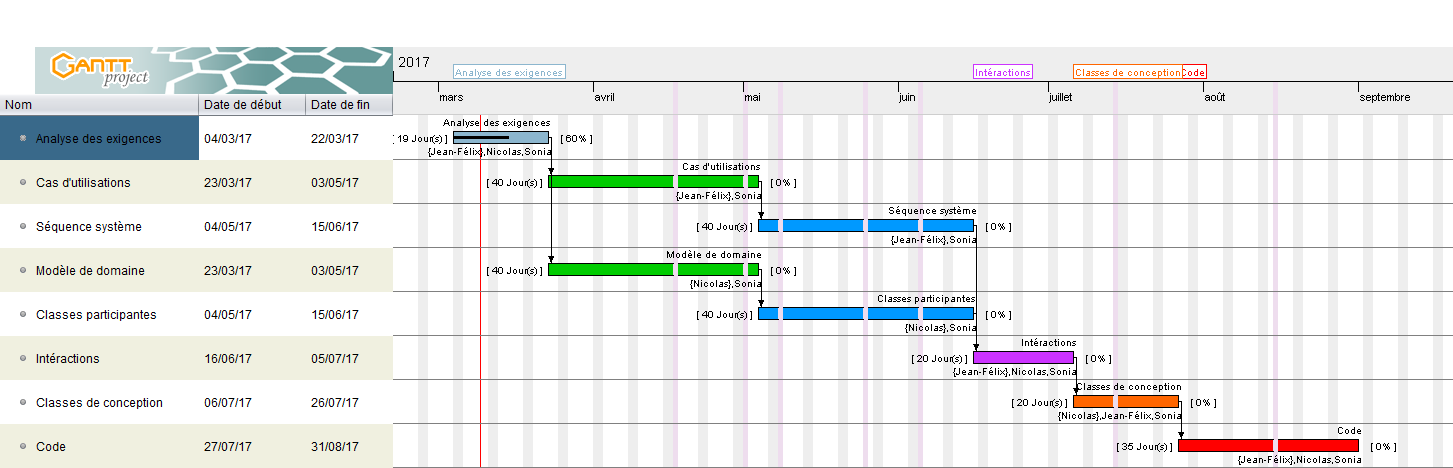
\includegraphics[width=1.0\textwidth]{Vitameal_gantt} %
\caption{Gantt}
\end{figure}

Le diagramme de PERT donne une autre vues de la répartition et de l'enchaînement des taches:
\begin{figure}[H]
\textbf{P}rogram \textbf{E}valuation and \textbf{R}eview \textbf{T}echnique
\label{PERT}
  \centering
      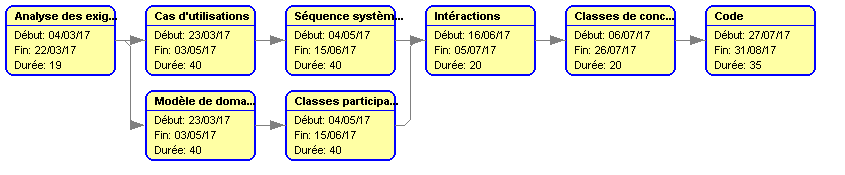
\includegraphics[width=1.0\textwidth]{Vitameal_pert} %
\caption{PERT}
\end{figure}

\subsection{Affectation des ressources}
Les ressources sont affectées comme suit:

\begin{tabular}{|l|l|}
\hiderowcolors
  \hline
  Tâches & Ressources \\ \hline
  Analyse des exigences & Nicolas, Sonia, Jean-Félix \\
  Cas d'utilisation & Jean-Félix 67\%, Sonia 33\% \\
  Modèle de domaine & Nicolas 67\%, Sonia 33\% \\
  Séquences système & Jean-Félix 67\%, Sonia 33\% \\
  Classes participantes & Nicolas 67\%, Sonia 33\% \\
  Diagramme d'interactions & Nicolas, Sonia, Jean-Félix \\
  Classes de conception & Nicolas, Sonia, Jean-Félix \\
  Code & Nicolas, Sonia, Jean-Félix \\ \hline
\end{tabular}

\begin{figure}[H]
\label{Ressources}
  \centering
      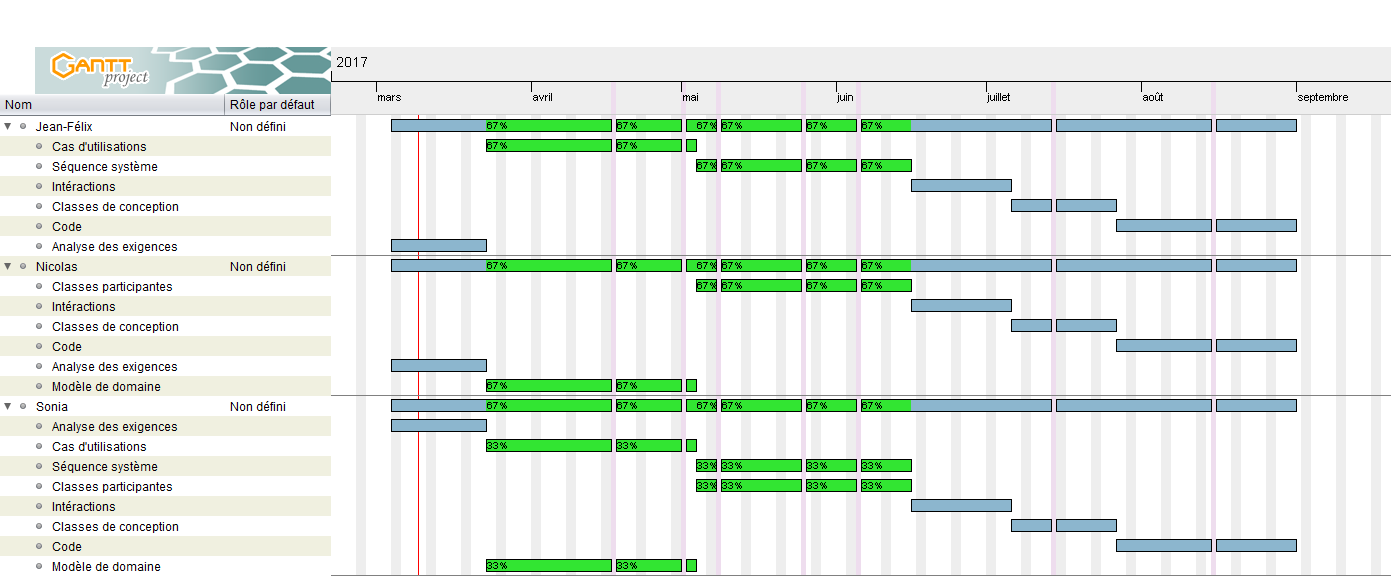
\includegraphics[width=1.0\textwidth]{Vitameal_ressources} %
\caption{Ressources}
\end{figure}

\section{Outils}

L'usine logicielle de Vitameal répond aux exigences suivantes :

\begin{itemize}
	\item respecter les règles de qualités ;
	\item avoir une documentation claire et intégrée au projet ;
	\item gérer les erreurs et assurer leurs suivies ;
	\item versionnionner le code source et la documentation ;
	\item avoir un espace commun accessible à distance ;
	\item gérer un espace de livraison générant des indicateurs de santé sur le projet ;
	\item avoir un outil de conception UML couvrant la methode minimal UML ;
	\item gérer la planification du projet.
\end{itemize}

\subsection{Outils utilisés}

Les outils utilisés par l'usine logicielle de Vitameal se sépare en deux catégories :

\begin{itemize}
	\item Le côté poste de développement qui correspond aux outils installés par chaque développeur sur sa machine ;
	\item Le côté espace d'intégration continue et de gestion de projet qui correspond aux outils composant l'espace communs de collaborations.
\end{itemize}

La documentation du projet est assurée par l'utilisation de la syntaxe \emph{markdown} intégrée à l'outil \emph{GitHub} et le langage de génération des livrables est \emph{LaTex}.

Le langage cible de cette usine est Java, mais elle peut facilement être adaptée à d'autre langage.

\subsubsection{Côté poste de développement}

\begin{itemize}
	\item \textbf{Eclipse} comme IDE pour écrire/éditer le code de l'application ;
	\item \textbf{Maven} comme constructeur du projet (gestion des dépendances, automatisation de la construction ;
	\item \textbf{JUnit} pour écrire les tests unitaires de l'application et \textbf{Codertura} pour analyser la couverture du projet par ces tests ;
	\item \textbf{Git} pour versionner les sources du projet ;
	\item \textbf{Papyrus} pour modéliser selon le standard UML le projet ;
	\item \textbf{GanttProject} pour planifier le projet avec un diagramme de Gantt ;
	\item \textbf{TEXMaker} pour éditer les fichiers\texttt{.tex} avec un comportement proche des \emph{WYSIWYG} (optionnel).
\end{itemize}

\subsubsection{Côté espace d'intégration continue et gestion de projet}

\begin{itemize}
	\item \textbf{GitHub} comme gestionnaire à distance du repositorie Git principal, comme tracker de bug et comme affichage visuel des taches à faire ;
	\item \textbf{Redmine} pour organiser le projet et rendre visible l'avancement du projet;
	\item \textbf{Jenkins} comme serveur d'intégration continue ;
	\item \textbf{SonarQube} comme analyseur de qualité du code.
\end{itemize}

\subsection{Schema de fonctionnement}

\begin{figure}[H]
	\label{Usine logicielle de Vitameal}
	\centering
	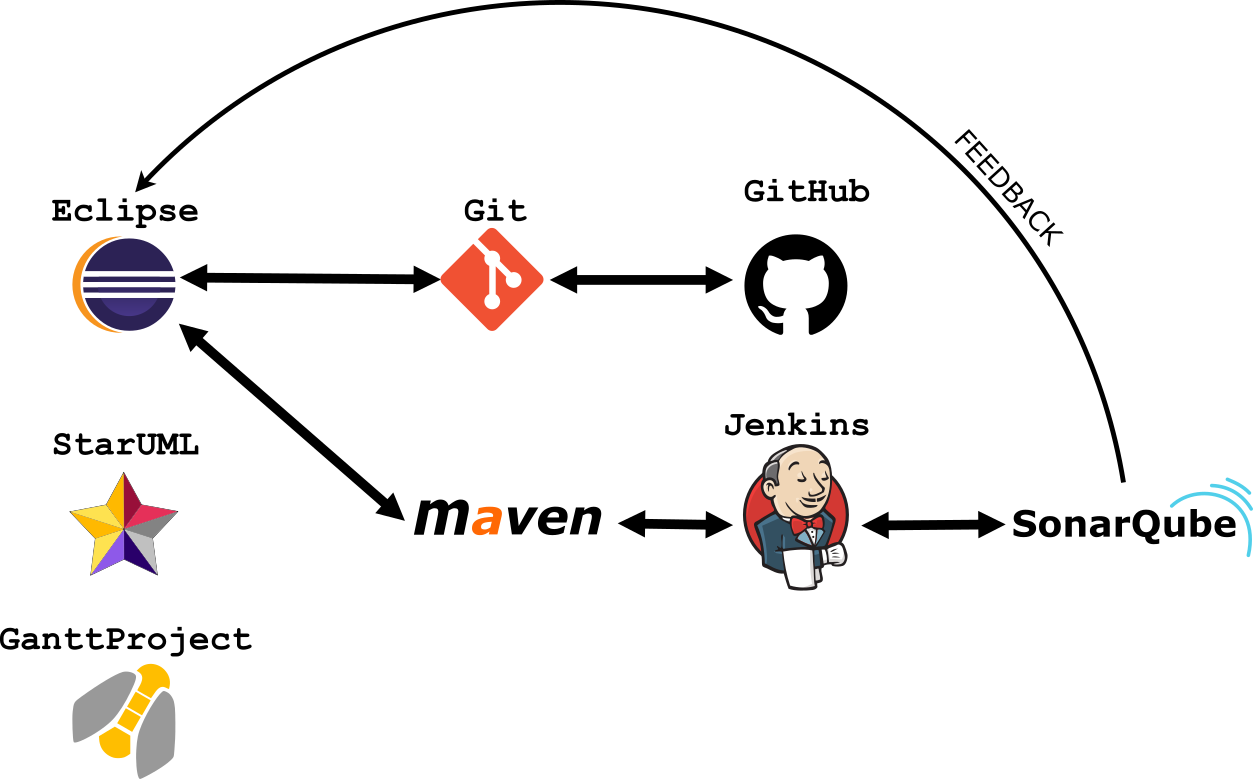
\includegraphics[width=0.8\textwidth]{usine_vitameal} %
	\caption{Usine logicielle de Vitameal}
\end{figure}


L'usine logicielle du projet Vitameal à pour porte d'entrée principale L'IDE  \textbf{Eclipse}, qui munis de plugins adéquat permet d'éditer la plupart des fichiers composants le projet.  
La collaboration sur le projet est assurée par le gestionnaire de version  \textbf{Git}, avec un repositorie central hébergé par \textbf{GitHub}.

Le  \textit{feedback} sur la santé du projet (qualité, couverture par les tests, build réussi, ...) est géré par le serveur d'intégration continue  \textbf{Jenkins}, utilisant \textbf{Maven} comme outils de configurations du projet et se branchant sur \textbf{SonarQube} pour obtenir les métriques.

L' outil  \textbf{Papyrus} est dédié à la conception UML de l'application, et l'outil  \textbf{Redmine} à la gestion de l'avancement du projet.

%\section{\colorbox{yellow}{TODO} Analyse}

%\section{\colorbox{yellow}{TODO} Vision détaillée}

%\section{\colorbox{yellow}{TODO} Cible}

%\section{\colorbox{yellow}{TODO} Risques}

%\section{\colorbox{yellow}{TODO} Besoins précis}

%\section{\colorbox{yellow}{TODO} Définition itérative de l'architecture}

%\section{\colorbox{yellow}{TODO} Estimation fine}

%-*- coding: utf-8 -*-
\textcolor[RGB]{46, 116, 181}{\chapter{Analyse des exigences}}
\section{Partie prenantes}
\begin{itemize}
\item Participantes~: les diététiciens, le service restauration
\item Concernés~: les médecins, la direction (budget)
\item Impactées~: les patients
\end{itemize}

\section{Les besoins}
\begin{description}
\item[] En tant que diététicien, j’ai besoin de :
\begin{description}
 \item[N001:] pouvoir renseigner le profil diététique des patients, afin qu’ils
 puissent bénéficier de menus adaptés.
 \item[N002:] pouvoir élaborer les menus des 3 repas journaliers
 (petit-déjeuner, déjeuner et dîner dont la composition est décrite en annexe
 \ref{annexeA}), de façon automatique, en tenant compte de grammages dépendant du type d'aliments et de la tranche d'age (Document \ref{docNutrition}, Annexe 2).
 \item[N003:] pouvoir saisir des plats et leur composition.
 \item[N004:] élaborer des menus selon les fréquences de service, selon le
 document \ref{docNutrition}, Annexe 4.
 \item[N005:] classer chaque aliment dans une des catégories d’aliments citée
 dans les tables de grammages du document \ref{docNutrition}, Annexes 2 et 4.
\end{description}
\item[N006:] En tant qu’administrateur du site internet de l’hôpital, j’ai
besoin de récupérer le menu de la semaine, afin pouvoir l’intégrer au site.
\item[N007:] En tant que médecin, j’ai besoin de consulter les profils
diététiques des patients admis, pour les  valider.
\item[N008:] En tant que cuisinier du service restauration, j’ai besoin de
consulter les menus élaborés, afin de pouvoir les préparer et prévoir les ingrédients à commander.
\item[N009:] En tant qu’agent de restauration hospitalière,  j’ai besoin de
connaître les menus de chaque patient, afin de pouvoir assembler les plateaux repas.
\end{description}
\section{Les contraintes}
\begin{description}
\item[N010:] Les médecins doivent pouvoir vérifier / valider les profils
diététiques des patients.
\item[N011:] La direction fixe un budget maximum par menu.
\end{description}

\section{Exigences}

\rowcolors{1}{}{}

\begin{table}[!h]

\begin{tabular}{|p{60mm}p{100mm}|}

\hline

\multicolumn{2}{|l|}{\textbf{REQ\_0100:} 3 repas} \\ \hline

\emph{Type:} Métier & \emph{Liens:} REQ\_0101 REQ\_0105  \\

\emph{Origine:}  & \emph{Validé:} Non \\

\emph{Version:} Initial & \emph{Test:}  \\

\emph{Priorité:} Must & \\ \hline

\multicolumn{2}{|p{16cm}|}{Le système doit permettre de concevoir les 3 repas (petit-déjeuner, déjeuner, souper) d'une journée.} \\ \hline

\end{tabular}

\end{table}



\begin{table}[!h]

\begin{tabular}{|p{60mm}p{100mm}|}

\hline

\multicolumn{2}{|l|}{\textbf{REQ\_0101:} Petit déjeuner} \\ \hline

\emph{Type:} Métier & \emph{Liens:} REQ\_0102 REQ\_0103 REQ\_0104  \\

\emph{Origine:}  & \emph{Validé:} Non \\

\emph{Version:} Initial & \emph{Test:}  \\

\emph{Priorité:} Should & \\ \hline

\multicolumn{2}{|p{16cm}|}{Le système doit permettre de concevoir un petit-déjeuner composé d'une boisson, d'un aliment céréalier, d'un produit laitier et d'un fruit.} \\ \hline

\end{tabular}

\end{table}



\begin{table}[!h]

\begin{tabular}{|p{60mm}p{100mm}|}

\hline

\multicolumn{2}{|l|}{\textbf{REQ\_0102:} Éléments petit déjeuner} \\ \hline

\emph{Type:} Métier & \emph{Liens:}  \\

\emph{Origine:}  & \emph{Validé:} Non \\

\emph{Version:} Initial & \emph{Test:}  \\

\emph{Priorité:} Must & \\ \hline

\multicolumn{2}{|p{16cm}|}{Le système doit permettre de rajouter au petit déjeuner un élément lipidique, sucré ou protodique.} \\ \hline

\end{tabular}

\end{table}



\begin{table}[!h]

\begin{tabular}{|p{60mm}p{100mm}|}

\hline

\multicolumn{2}{|l|}{\textbf{REQ\_0103:} Éléments non diététiques} \\ \hline

\emph{Type:} Métier & \emph{Liens:}  \\

\emph{Origine:}  & \emph{Validé:} Non \\

\emph{Version:} Initial & \emph{Test:}  \\

\emph{Priorité:} Should & \\ \hline

\multicolumn{2}{|p{16cm}|}{Le système doit avertir l'utilisateur de l'usage d'élément non diététique dans un petit déjeuner.} \\ \hline

\end{tabular}

\end{table}



\begin{table}[!h]

\begin{tabular}{|p{60mm}p{100mm}|}

\hline

\multicolumn{2}{|l|}{\textbf{REQ\_0104:} Fréquence éléments non diététiques} \\ \hline

\emph{Type:} Métier & \emph{Liens:}  \\

\emph{Origine:}  & \emph{Validé:} Non \\

\emph{Version:} Initial & \emph{Test:}  \\

\emph{Priorité:} Should & \\ \hline

\multicolumn{2}{|p{16cm}|}{Le système doit vérifier que la fréquence de l'usage d'élément non diététique des petits déjeuners ne dépasse pas 3 repas sur 20, il avertit l'utilisateur si c'est le cas.} \\ \hline

\end{tabular}

\end{table}



\begin{table}[!h]

\begin{tabular}{|p{60mm}p{100mm}|}

\hline

\multicolumn{2}{|l|}{\textbf{REQ\_0105:} Composition déjeuner} \\ \hline

\emph{Type:} Métier & \emph{Liens:}  \\

\emph{Origine:}  & \emph{Validé:} Non \\

\emph{Version:} Initial & \emph{Test:}  \\

\emph{Priorité:} Must & \\ \hline

\multicolumn{2}{|p{16cm}|}{Le système de concevoir un déjeuner et souper composés de 4 ou cinq composantes parmi : entrée, plat protodique, garniture, produit, laitier desserts + de l'eau et du pain (selon le tableau sur la composition du déjeuner en annexe A).} \\ \hline

\end{tabular}

\end{table}



\begin{table}[!h]

\begin{tabular}{|p{60mm}p{100mm}|}

\hline

\multicolumn{2}{|l|}{\textbf{REQ\_0106:} Ajout de plats} \\ \hline

\emph{Type:} Métier & \emph{Liens:}  \\

\emph{Origine:}  & \emph{Validé:} Non \\

\emph{Version:} Initial & \emph{Test:}  \\

\emph{Priorité:} Must & \\ \hline

\multicolumn{2}{|p{16cm}|}{Le système doit permettre d'ajouter des plats et leur définition dans la listes des plats pouvant être préparés.} \\ \hline

\end{tabular}

\end{table}



\begin{table}[!h]

\begin{tabular}{|p{60mm}p{100mm}|}

\hline

\multicolumn{2}{|l|}{\textbf{REQ\_0107:} Description d'un plat} \\ \hline

\emph{Type:} Métier & \emph{Liens:}  \\

\emph{Origine:}  & \emph{Validé:} Non \\

\emph{Version:} Initial & \emph{Test:}  \\

\emph{Priorité:} Must & \\ \hline

\multicolumn{2}{|p{16cm}|}{Le système doit permettre la description d'un plat avec sa liste d'ingrédients et les quantités nécessaires à sa réalisation.} \\ \hline

\end{tabular}

\end{table}



\begin{table}[!h]

\begin{tabular}{|p{60mm}p{100mm}|}

\hline

\multicolumn{2}{|l|}{\textbf{REQ\_0108:} Fréquence de service} \\ \hline

\emph{Type:} Métier & \emph{Liens:}  \\

\emph{Origine:}  & \emph{Validé:} Non \\

\emph{Version:} Initial & \emph{Test:}  \\

\emph{Priorité:} Must & \\ \hline

\multicolumn{2}{|p{16cm}|}{Le système doit proposer un plat selon la fréquence de service de ce plat (exemple 4 fois tous les 20 repas).} \\ \hline

\end{tabular}

\end{table}



\begin{table}[!h]

\begin{tabular}{|p{60mm}p{100mm}|}

\hline

\multicolumn{2}{|l|}{\textbf{REQ\_0410:} Composants des repas} \\ \hline

\emph{Type:} Métier & \emph{Liens:}  \\

\emph{Origine:}  & \emph{Validé:} Non \\

\emph{Version:} Initial & \emph{Test:}  \\

\emph{Priorité:} Must & \\ \hline

\multicolumn{2}{|p{16cm}|}{Le système doit permettre d'ajouter et de supprimer des éléments dans les composants des repas.} \\ \hline

\end{tabular}

\end{table}



\begin{table}[!h]

\begin{tabular}{|p{60mm}p{100mm}|}

\hline

\multicolumn{2}{|l|}{\textbf{REQ\_0411:} Listes par défaut} \\ \hline

\emph{Type:} Métier & \emph{Liens:}  \\

\emph{Origine:}  & \emph{Validé:} Non \\

\emph{Version:} Initial & \emph{Test:}  \\

\emph{Priorité:} Should & \\ \hline

\multicolumn{2}{|p{16cm}|}{Le système doit permettre de revenir aux listes par défaut recommandé par le gouvernement.} \\ \hline

\end{tabular}

\end{table}



\begin{table}[!h]

\begin{tabular}{|p{60mm}p{100mm}|}

\hline

\multicolumn{2}{|l|}{\textbf{REQ\_0500:} Fiche de commande} \\ \hline

\emph{Type:} Métier & \emph{Liens:}  \\

\emph{Origine:}  & \emph{Validé:} Non \\

\emph{Version:} Initial & \emph{Test:}  \\

\emph{Priorité:} Could & \\ \hline

\multicolumn{2}{|p{16cm}|}{Le système doit permettre, une fois les menus élaborés de générer un fiche de commande au format : à définir.} \\ \hline

\end{tabular}

\end{table}



\begin{table}[!h]

\begin{tabular}{|p{60mm}p{100mm}|}

\hline

\multicolumn{2}{|l|}{\textbf{REQ\_0501:} Publication menus} \\ \hline

\emph{Type:} Non Fonctionnelle & \emph{Liens:}  \\

\emph{Origine:}  & \emph{Validé:} Non \\

\emph{Version:} Initial & \emph{Test:}  \\

\emph{Priorité:} Could & \\ \hline

\multicolumn{2}{|p{16cm}|}{Le système doit permettre d'afficher les menus sur un site internet.} \\ \hline

\end{tabular}

\end{table}



\begin{table}[!h]

\begin{tabular}{|p{60mm}p{100mm}|}

\hline

\multicolumn{2}{|l|}{\textbf{REQ\_0600:} Validation des repas} \\ \hline

\emph{Type:} Contrainte & \emph{Liens:}  \\

\emph{Origine:}  & \emph{Validé:} Non \\

\emph{Version:} Initial & \emph{Test:}  \\

\emph{Priorité:} Must & \\ \hline

\multicolumn{2}{|p{16cm}|}{Le système doit gérer un cycle de validation des repas : en cours d'élaboration, en attente de validation, validé.} \\ \hline

\end{tabular}

\end{table}



\begin{table}[!h]

\begin{tabular}{|p{60mm}p{100mm}|}

\hline

\multicolumn{2}{|l|}{\textbf{REQ\_0601:} Droits utilisateurs} \\ \hline

\emph{Type:} Contrainte & \emph{Liens:}  \\

\emph{Origine:}  & \emph{Validé:} Non \\

\emph{Version:} Initial & \emph{Test:}  \\

\emph{Priorité:} Must & \\ \hline

\multicolumn{2}{|p{16cm}|}{Le système doit permettre de gérer différent droit selon le type d'utilisateur.} \\ \hline

\end{tabular}

\end{table}



\begin{table}[!h]

\begin{tabular}{|p{60mm}p{100mm}|}

\hline

\multicolumn{2}{|l|}{\textbf{REQ\_0700:} Menus à assembler} \\ \hline

\emph{Type:} Métier & \emph{Liens:}  \\

\emph{Origine:}  & \emph{Validé:} Non \\

\emph{Version:} Initial & \emph{Test:}  \\

\emph{Priorité:} Must & \\ \hline

\multicolumn{2}{|p{16cm}|}{Le système doit afficher les menu à assembler pour un jour donnée et émettre une étiquette au format : à définir.} \\ \hline

\end{tabular}

\end{table}



\begin{table}[!h]

\begin{tabular}{|p{60mm}p{100mm}|}

\hline

\multicolumn{2}{|l|}{\textbf{REQ\_0701:} Limite prix repas} \\ \hline

\emph{Type:} Contrainte & \emph{Liens:}  \\

\emph{Origine:}  & \emph{Validé:} Non \\

\emph{Version:} Initial & \emph{Test:}  \\

\emph{Priorité:} Must & \\ \hline

\multicolumn{2}{|p{16cm}|}{Le système doit permettre de fixer une limite au prix d'un repas.} \\ \hline

\end{tabular}

\end{table}



\begin{table}[!h]

\begin{tabular}{|p{60mm}p{100mm}|}

\hline

\multicolumn{2}{|l|}{\textbf{REQ\_0702:} Prix repas} \\ \hline

\emph{Type:} Métier & \emph{Liens:}  \\

\emph{Origine:}  & \emph{Validé:} Non \\

\emph{Version:} Initial & \emph{Test:}  \\

\emph{Priorité:} Must & \\ \hline

\multicolumn{2}{|p{16cm}|}{Le système doit permettre de renseigner le prix des éléments d'un repas.} \\ \hline

\end{tabular}

\end{table}



\begin{table}[!h]

\begin{tabular}{|p{60mm}p{100mm}|}

\hline

\multicolumn{2}{|l|}{\textbf{REQ\_0902:} Profil patient} \\ \hline

\emph{Type:} Métier & \emph{Liens:}  \\

\emph{Origine:}  & \emph{Validé:} Non \\

\emph{Version:} Initial & \emph{Test:}  \\

\emph{Priorité:} Must & \\ \hline

\multicolumn{2}{|p{16cm}|}{Le système doit permettre de renseigner un profil patient comportant les éléments suivants : regime particulier(liste à définir), allergie(liste à définir), contre-indication (liste à définir).} \\ \hline

\end{tabular}

\end{table}



\begin{table}[!h]

\begin{tabular}{|p{60mm}p{100mm}|}

\hline

\multicolumn{2}{|l|}{\textbf{REQ\_1000:} État civil} \\ \hline

\emph{Type:} Métier & \emph{Liens:}  \\

\emph{Origine:}  & \emph{Validé:} Non \\

\emph{Version:} Initial & \emph{Test:}  \\

\emph{Priorité:} Must & \\ \hline

\multicolumn{2}{|p{16cm}|}{Le système doit permettre de renseigner l'état civil d'un patient.} \\ \hline

\end{tabular}

\end{table}



\begin{table}[!h]

\begin{tabular}{|p{60mm}p{100mm}|}

\hline

\multicolumn{2}{|l|}{\textbf{REQ\_1001:} Localisation patient} \\ \hline

\emph{Type:} Métier & \emph{Liens:}  \\

\emph{Origine:}  & \emph{Validé:} Non \\

\emph{Version:} Initial & \emph{Test:}  \\

\emph{Priorité:} Must & \\ \hline

\multicolumn{2}{|p{16cm}|}{Le système doit permettre de renseigner la localisation particulière d'un patient.} \\ \hline

\end{tabular}

\end{table}



\begin{table}[!h]

\begin{tabular}{|p{60mm}p{100mm}|}

\hline

\multicolumn{2}{|l|}{\textbf{REQ\_1002:} Grammages} \\ \hline

\emph{Type:} Métier & \emph{Liens:}  \\

\emph{Origine:}  & \emph{Validé:} Non \\

\emph{Version:} Initial & \emph{Test:}  \\

\emph{Priorité:} Must & \\ \hline

\multicolumn{2}{|p{16cm}|}{Le système doit permettre de gérer les grammage de plat.} \\ \hline

\end{tabular}

\end{table}



\begin{table}[!h]

\begin{tabular}{|p{60mm}p{100mm}|}

\hline

\multicolumn{2}{|l|}{\textbf{REQ\_1003:} Plateaux repas} \\ \hline

\emph{Type:} Métier & \emph{Liens:}  \\

\emph{Origine:}  & \emph{Validé:} Non \\

\emph{Version:} Initial & \emph{Test:}  \\

\emph{Priorité:} Must & \\ \hline

\multicolumn{2}{|p{16cm}|}{Le système doit pouvoir gérer des plateaux repas de type : sans régime particulier ou avec régime particulier.} \\ \hline

\end{tabular}

\end{table}



\begin{table}[!h]

\begin{tabular}{|p{60mm}p{100mm}|}

\hline

\multicolumn{2}{|l|}{\textbf{REQ\_1004:} Groupes} \\ \hline

\emph{Type:} Métier & \emph{Liens:}  \\

\emph{Origine:}  & \emph{Validé:} Non \\

\emph{Version:} Initial & \emph{Test:}  \\

\emph{Priorité:} Should & \\ \hline

\multicolumn{2}{|p{16cm}|}{Le système doit gérer les patients par groupes selon leur régime, exemple le groupe des intolérant au lactose.} \\ \hline

\end{tabular}

\end{table}



\begin{table}[!h]

\begin{tabular}{|p{60mm}p{100mm}|}

\hline

\multicolumn{2}{|l|}{\textbf{REQ\_1005:} Génération automatique} \\ \hline

\emph{Type:} Fonctionnelle & \emph{Liens:}  \\

\emph{Origine:}  & \emph{Validé:} Non \\

\emph{Version:} Initial & \emph{Test:}  \\

\emph{Priorité:} Must & \\ \hline

\multicolumn{2}{|p{16cm}|}{Le système doit permettre de générer automatiquement les repas pour un groupe de patients particulier.} \\ \hline

\end{tabular}

\end{table}



\begin{table}[!h]

\begin{tabular}{|p{60mm}p{100mm}|}

\hline

\multicolumn{2}{|l|}{\textbf{REQ\_1006:} Titre} \\ \hline

\emph{Type:} Utilisateur & \emph{Liens:}  \\

\emph{Origine:} Origine & \emph{Validé:} Oui \\

\emph{Version:} Initial & \emph{Test:} Test \\

\emph{Priorité:} Must & \\ \hline

\multicolumn{2}{|p{16cm}|}{le système doit stocker les fiches patients, et permettre de les modifier ou supprimer le cas échéant.} \\ \hline

\end{tabular}

\end{table}



\begin{table}[!h]

\begin{tabular}{|p{60mm}p{100mm}|}

\hline

\multicolumn{2}{|l|}{\textbf{REQ\_1007:} Titre} \\ \hline

\emph{Type:} Utilisateur & \emph{Liens:}  \\

\emph{Origine:} Origine & \emph{Validé:} Oui \\

\emph{Version:} Initial & \emph{Test:} Test \\

\emph{Priorité:} Must & \\ \hline

\multicolumn{2}{|p{16cm}|}{Le système doit permettre de trier les plats par catégories.} \\ \hline

\end{tabular}

\end{table}



\begin{table}[!h]

\begin{tabular}{|p{60mm}p{100mm}|}

\hline

\multicolumn{2}{|l|}{\textbf{REQ\_1008:} Titre} \\ \hline

\emph{Type:} Utilisateur & \emph{Liens:}  \\

\emph{Origine:} Origine & \emph{Validé:} Oui \\

\emph{Version:} Initial & \emph{Test:} Test \\

\emph{Priorité:} Must & \\ \hline

\multicolumn{2}{|p{16cm}|}{Le système doit stocker les intitulés des plats, et permettre leur modification ou leur suppression.} \\ \hline

\end{tabular}

\end{table}






%-*- coding: utf-8 -*-
\textcolor[RGB]{46, 116, 181}{\chapter{Analyse fonctionnelle}}

\section{Cas d'utilisation}

Les acteurs humains pour le système Vitameal sont les suivants :

Le diététicien : la personne en charge de l'élaboration des menus servis aux patients. Pour cela il doit pouvoir composer les menus des 3 repas journaliers selon les contraintes médicales de chaque patients. Il peut remplir lui-même les profils diététiques des patients mais ceux-ci doivent être validé par un médecin.

Le médecin : la personne en charge du dossier médical des patients, qui valide les profils diététiques remplit par les diététiciens.
 
Le service restauration : Les personnes en charge de la préparation et de la commande des repas.

\begin{figure}[H]
\centering
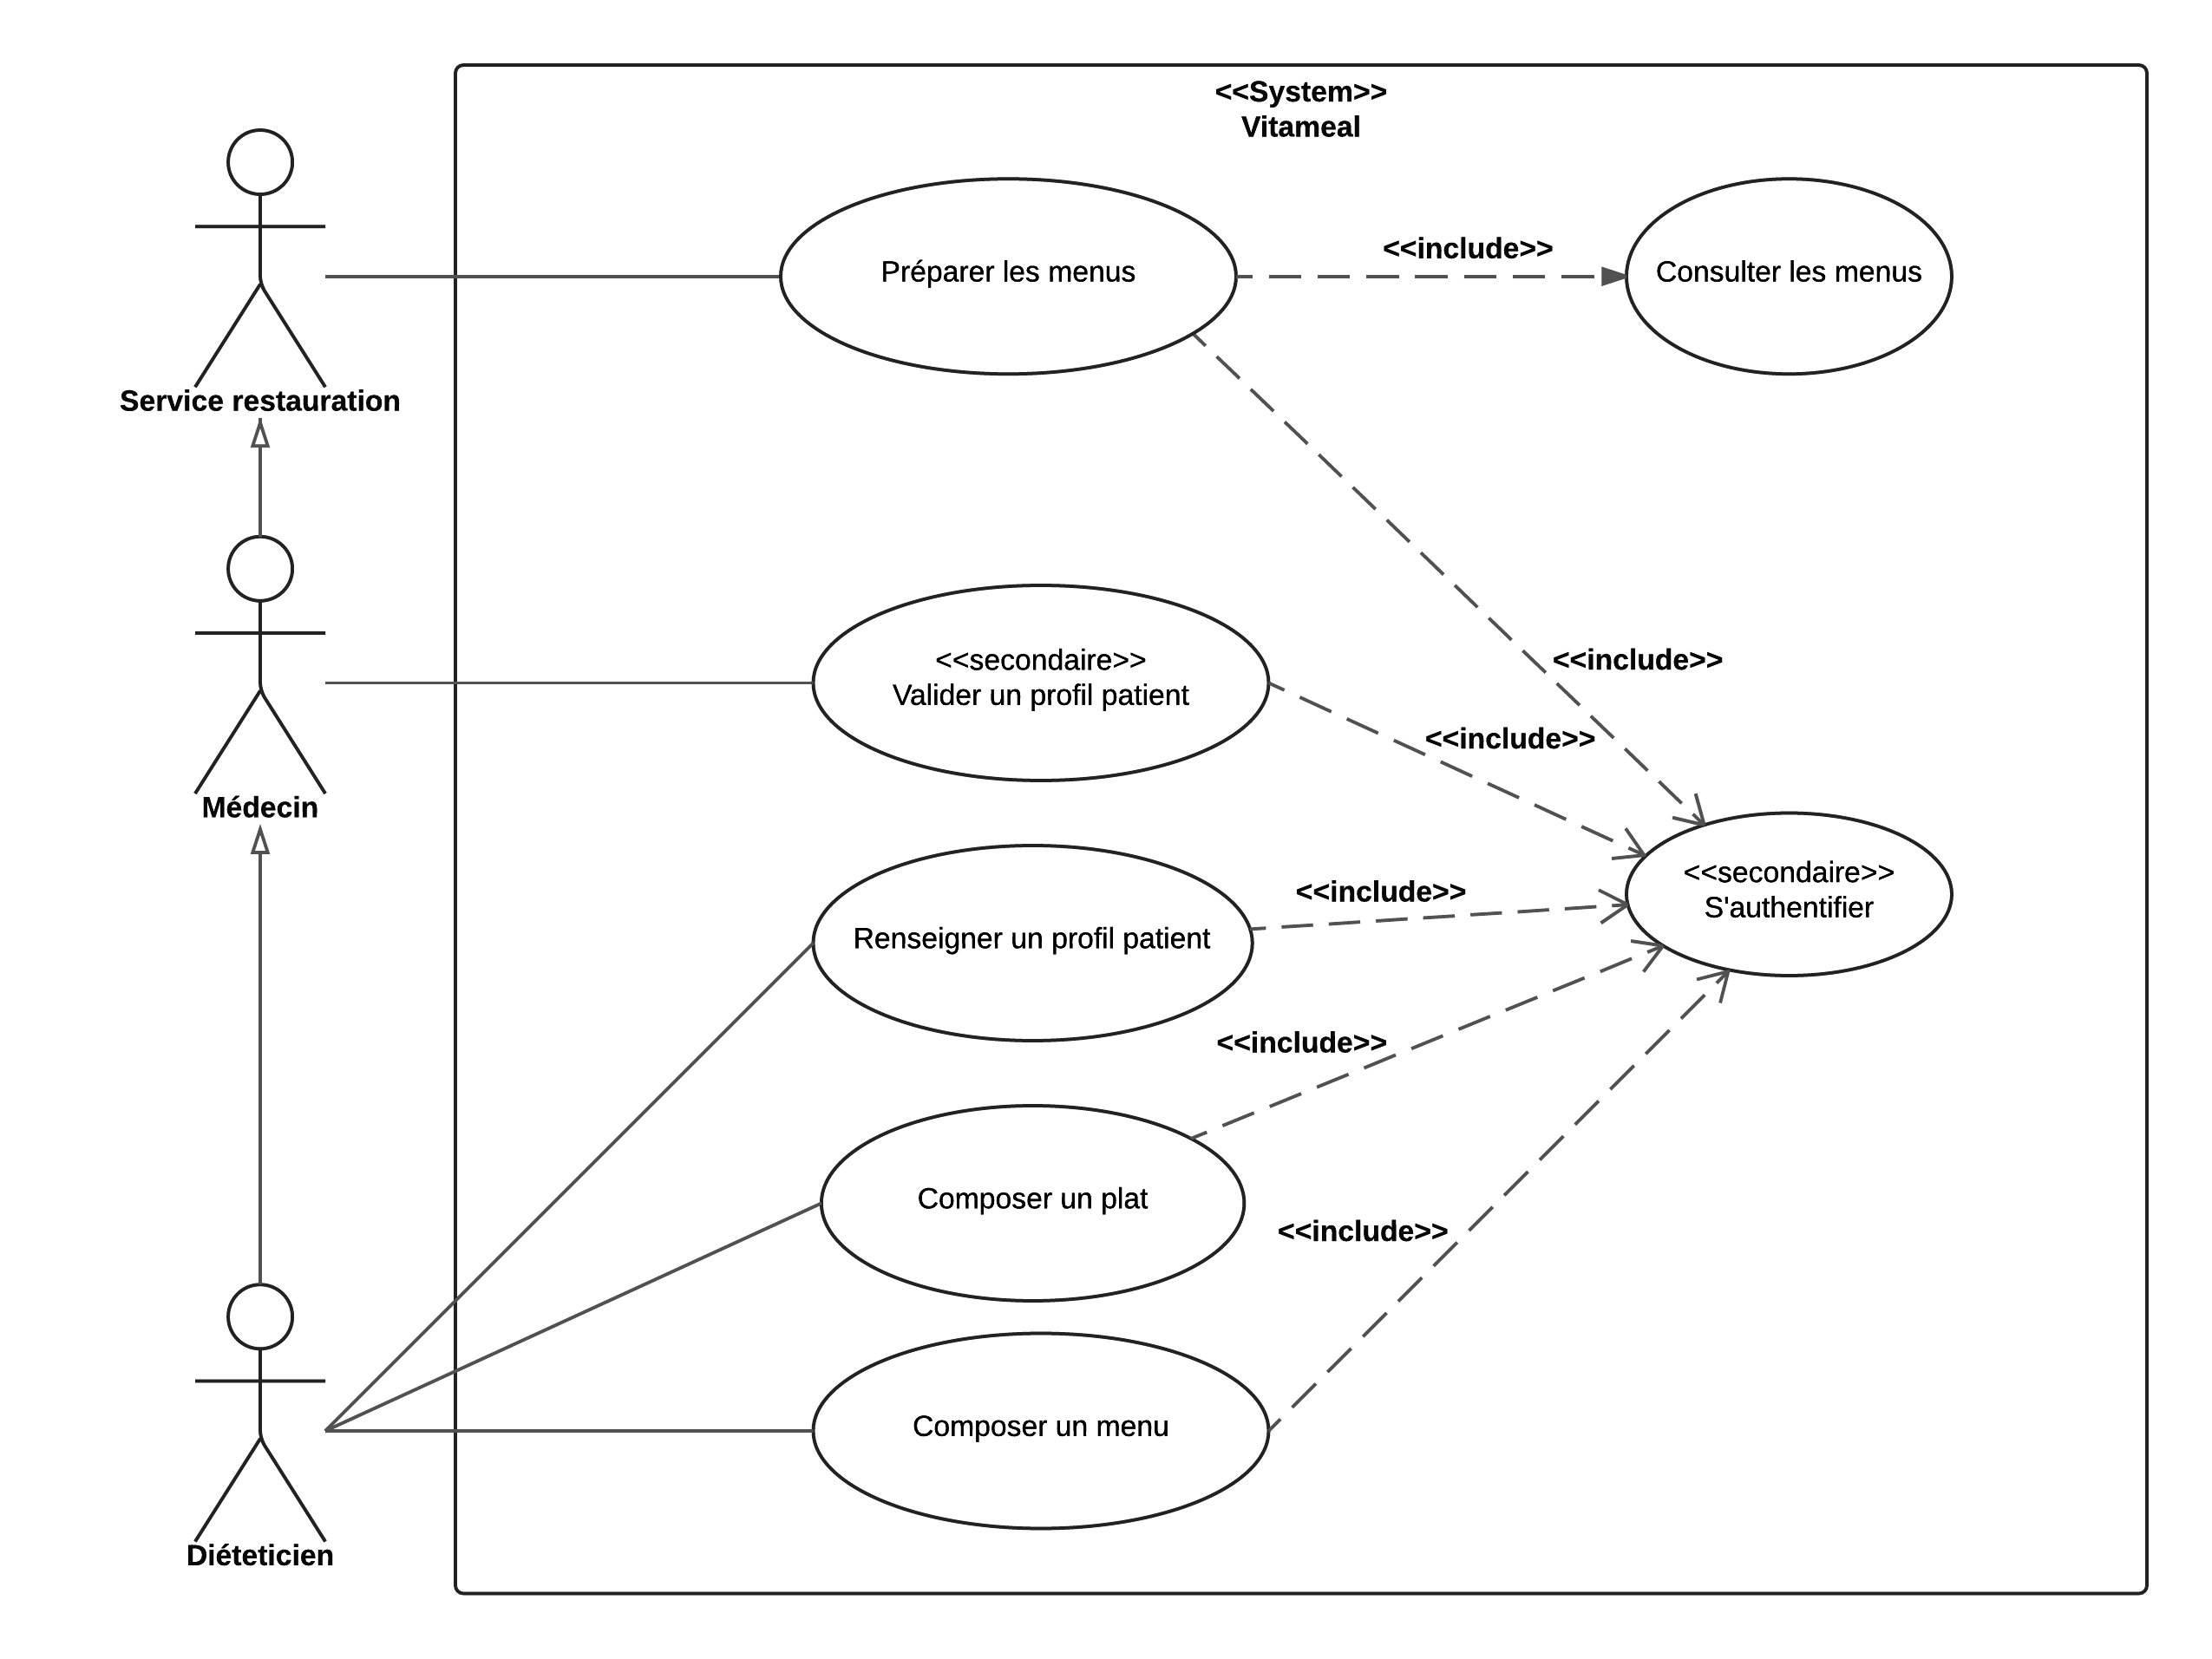
\includegraphics[scale=0.8]{../../CasDUtilisations/diagramme_cas_utilisation.png}
\caption{Diagramme des cas d'utilisation principal}
\end{figure}

Le stéréotype ``secondaire'' dans le diagramme des cas d'utilisation principal indique que le cas d'utilisation ne fait pas partie des cas d'utilisation principaux et qu'il n'est pas obligatoire pour que le système fonctionne.

\section{Description des cas d'utilisation}

\subsubsection{Préparer les menus}

\noindent\textbf{Nom :} Préparer les menus \\
\textbf{ID :} UC101 \\
\textbf{Description :} Le service restauration souhaite pouvoir préparé les menus par groupe de patient. \\
\textbf{Auteur :} Nicolas SYMPHORIEN \\
\textbf{Dates(s) :} 12/06/2017 \\
\textbf{Acteurs :} Le service restauration \\
\textbf{Pré-condition :} L'utilisateur a consulté les menus d'un groupe de patient (voir cas d'utilisation ''consulter les menus`` ).

\noindent \textbf{Scénario principal : } Figure \ref{PreparerMenuSeq}

\begin{enumerate}
	\item Le service restauration choisi les plat d'un jour qu'il veut préparer.
	\item Le système affiche la composition des plat du jour choisi avec les quantités pour chaque ingrédients
	\item Le service restauration peut choisir d'élaborer les plats d'un autre jour , dans ce cas le cas d'utilisation reprend à l'étape 1, sinon le cas d'utilisation se termine.
\end{enumerate}

\noindent \textbf{Post-Conditions:} Le service restauration a préparé tous les plats des jours qu'il souhaite.

\begin{figure}
\centering
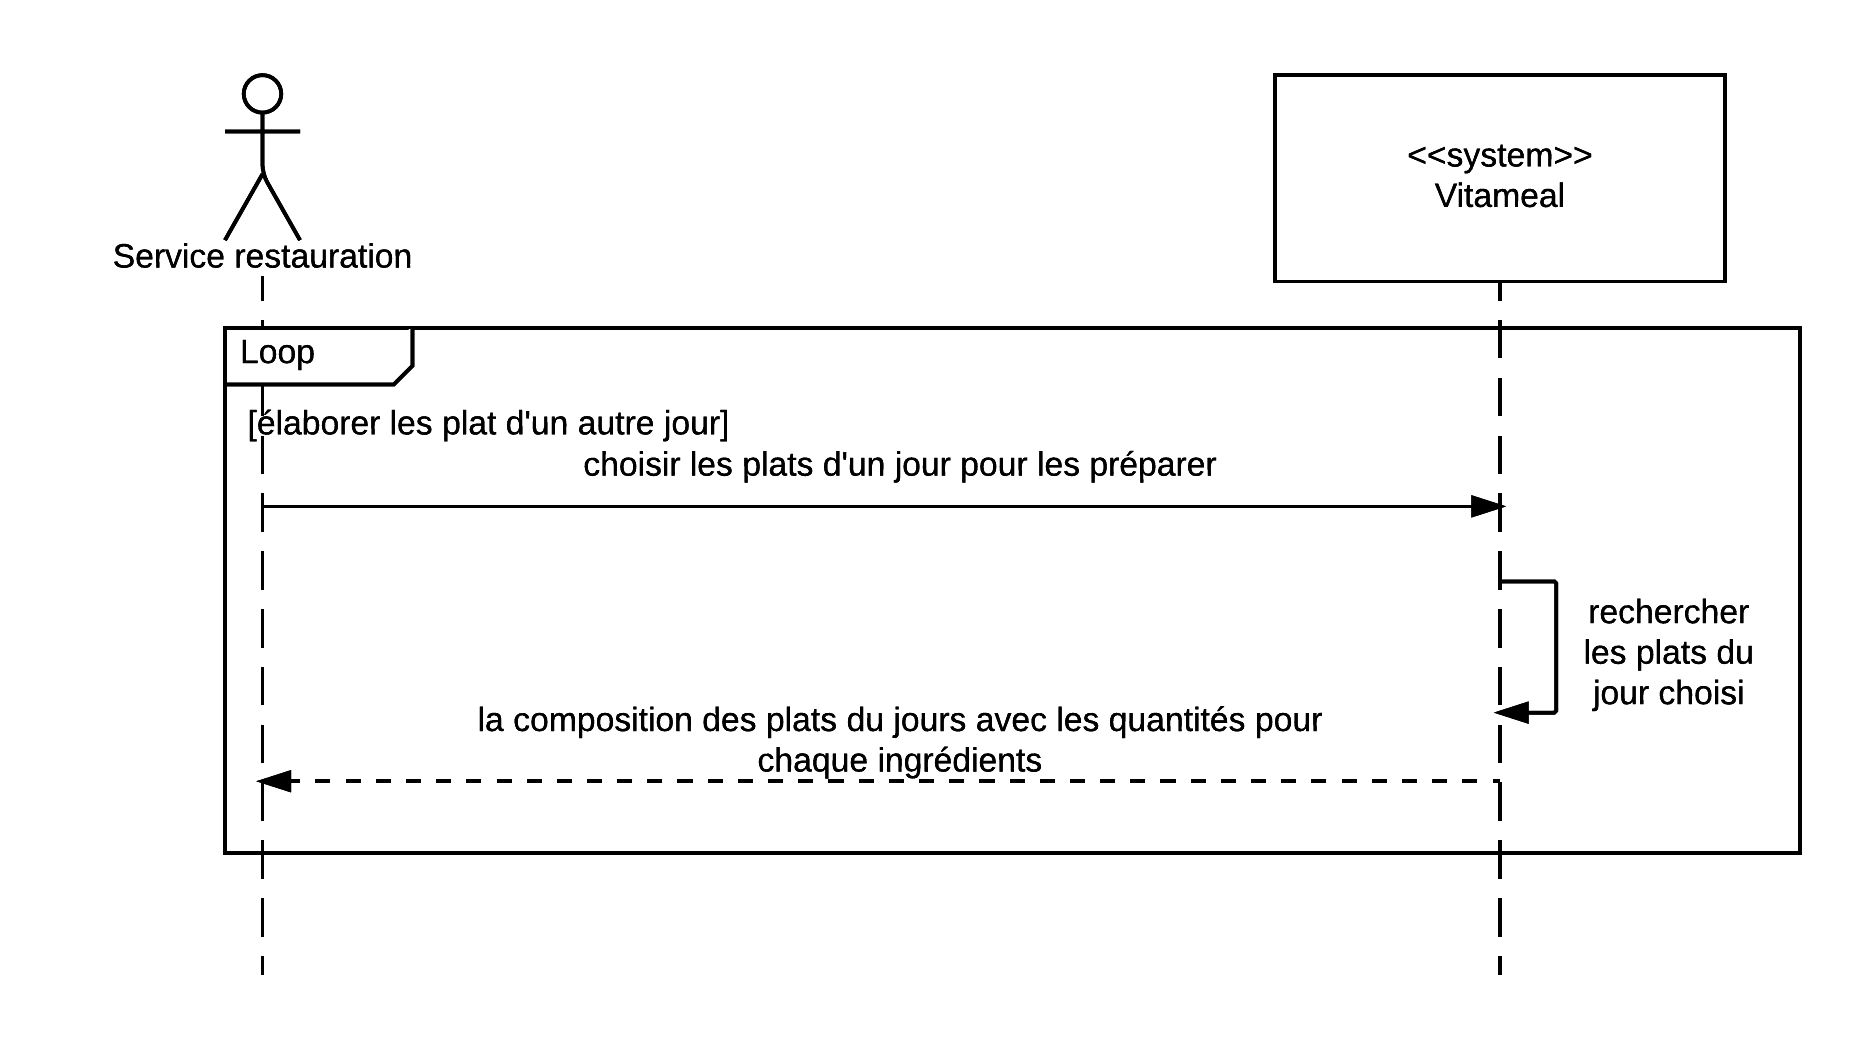
\includegraphics{../../CasDUtilisations/PreparerMenus/sequence_preparer_menus.png}
\caption{Diagramme de séquence du cas d'utilisation préparer les menus}
\label{PreparerMenuSeq}
\end{figure}

\subsection{Consulter les menus}

\noindent\textbf{Nom :} Consulter les menus \\
\textbf{ID :} UC102 \\
\textbf{Description :} Le service restauration souhaite pouvoir consulté les menus par groupe de patient. \\
\textbf{Auteur :} Nicolas SYMPHORIEN \\
\textbf{Dates(s) :} 11/06/2017 \\
\textbf{Acteurs :} Le service restauration \\
\textbf{Pré-condition :} L'utilisateur doit être identifié.

\noindent \textbf{Scénario principal :} Figure \ref{ConsulterMenusSeq}

\begin{enumerate}
	\item \label{UC102_step1}Le service restauration choisi le groupe de patient pour lequel il veut voir le menu.
	\item \label{UC102_step2}Le système affiche le menu de la semaine en cours selon le groupe de patient choisi
	\item \label{UC102_step3}Le service restauration peut choisir de consulter le menu pour un autre groupe de patient, dans ce cas le cas d'utilisation reprend à l'étape \ref{UC102_step1}, sinon le cas d'utilisation se termine.
\end{enumerate}

\noindent \textbf{Scénario alternatif :}

\textit{Premier scénario alternatif :}
Le scénario alternatif suivant débute après l'étape \ref{UC102_step2} du scénario nominal
\begin{enumerate}
	\item L'utilisateur peut changer de groupe de patient et le cas d'utilisation reprend à l'étape \ref{UC102_step2} du scénario nominal
\end{enumerate}

\textit{Second scénario alternatif :}
Le scénario alternatif suivant débute après l'étape \ref{UC102_step2} du scénario nominal
\begin{enumerate}
	\item Le service restauration peut changer de semaine
	\item Le système affiche le menu de la semaine choisi si il existe, sinon il affiche un message. 
\end{enumerate}
Le cas d'utilisation reprend à l'étape \ref{UC102_step3} du scénario nominal.

\noindent \textbf{Post-Conditions:} Le menu est affiché pour le groupe de patient choisi.

\begin{figure}
\centering
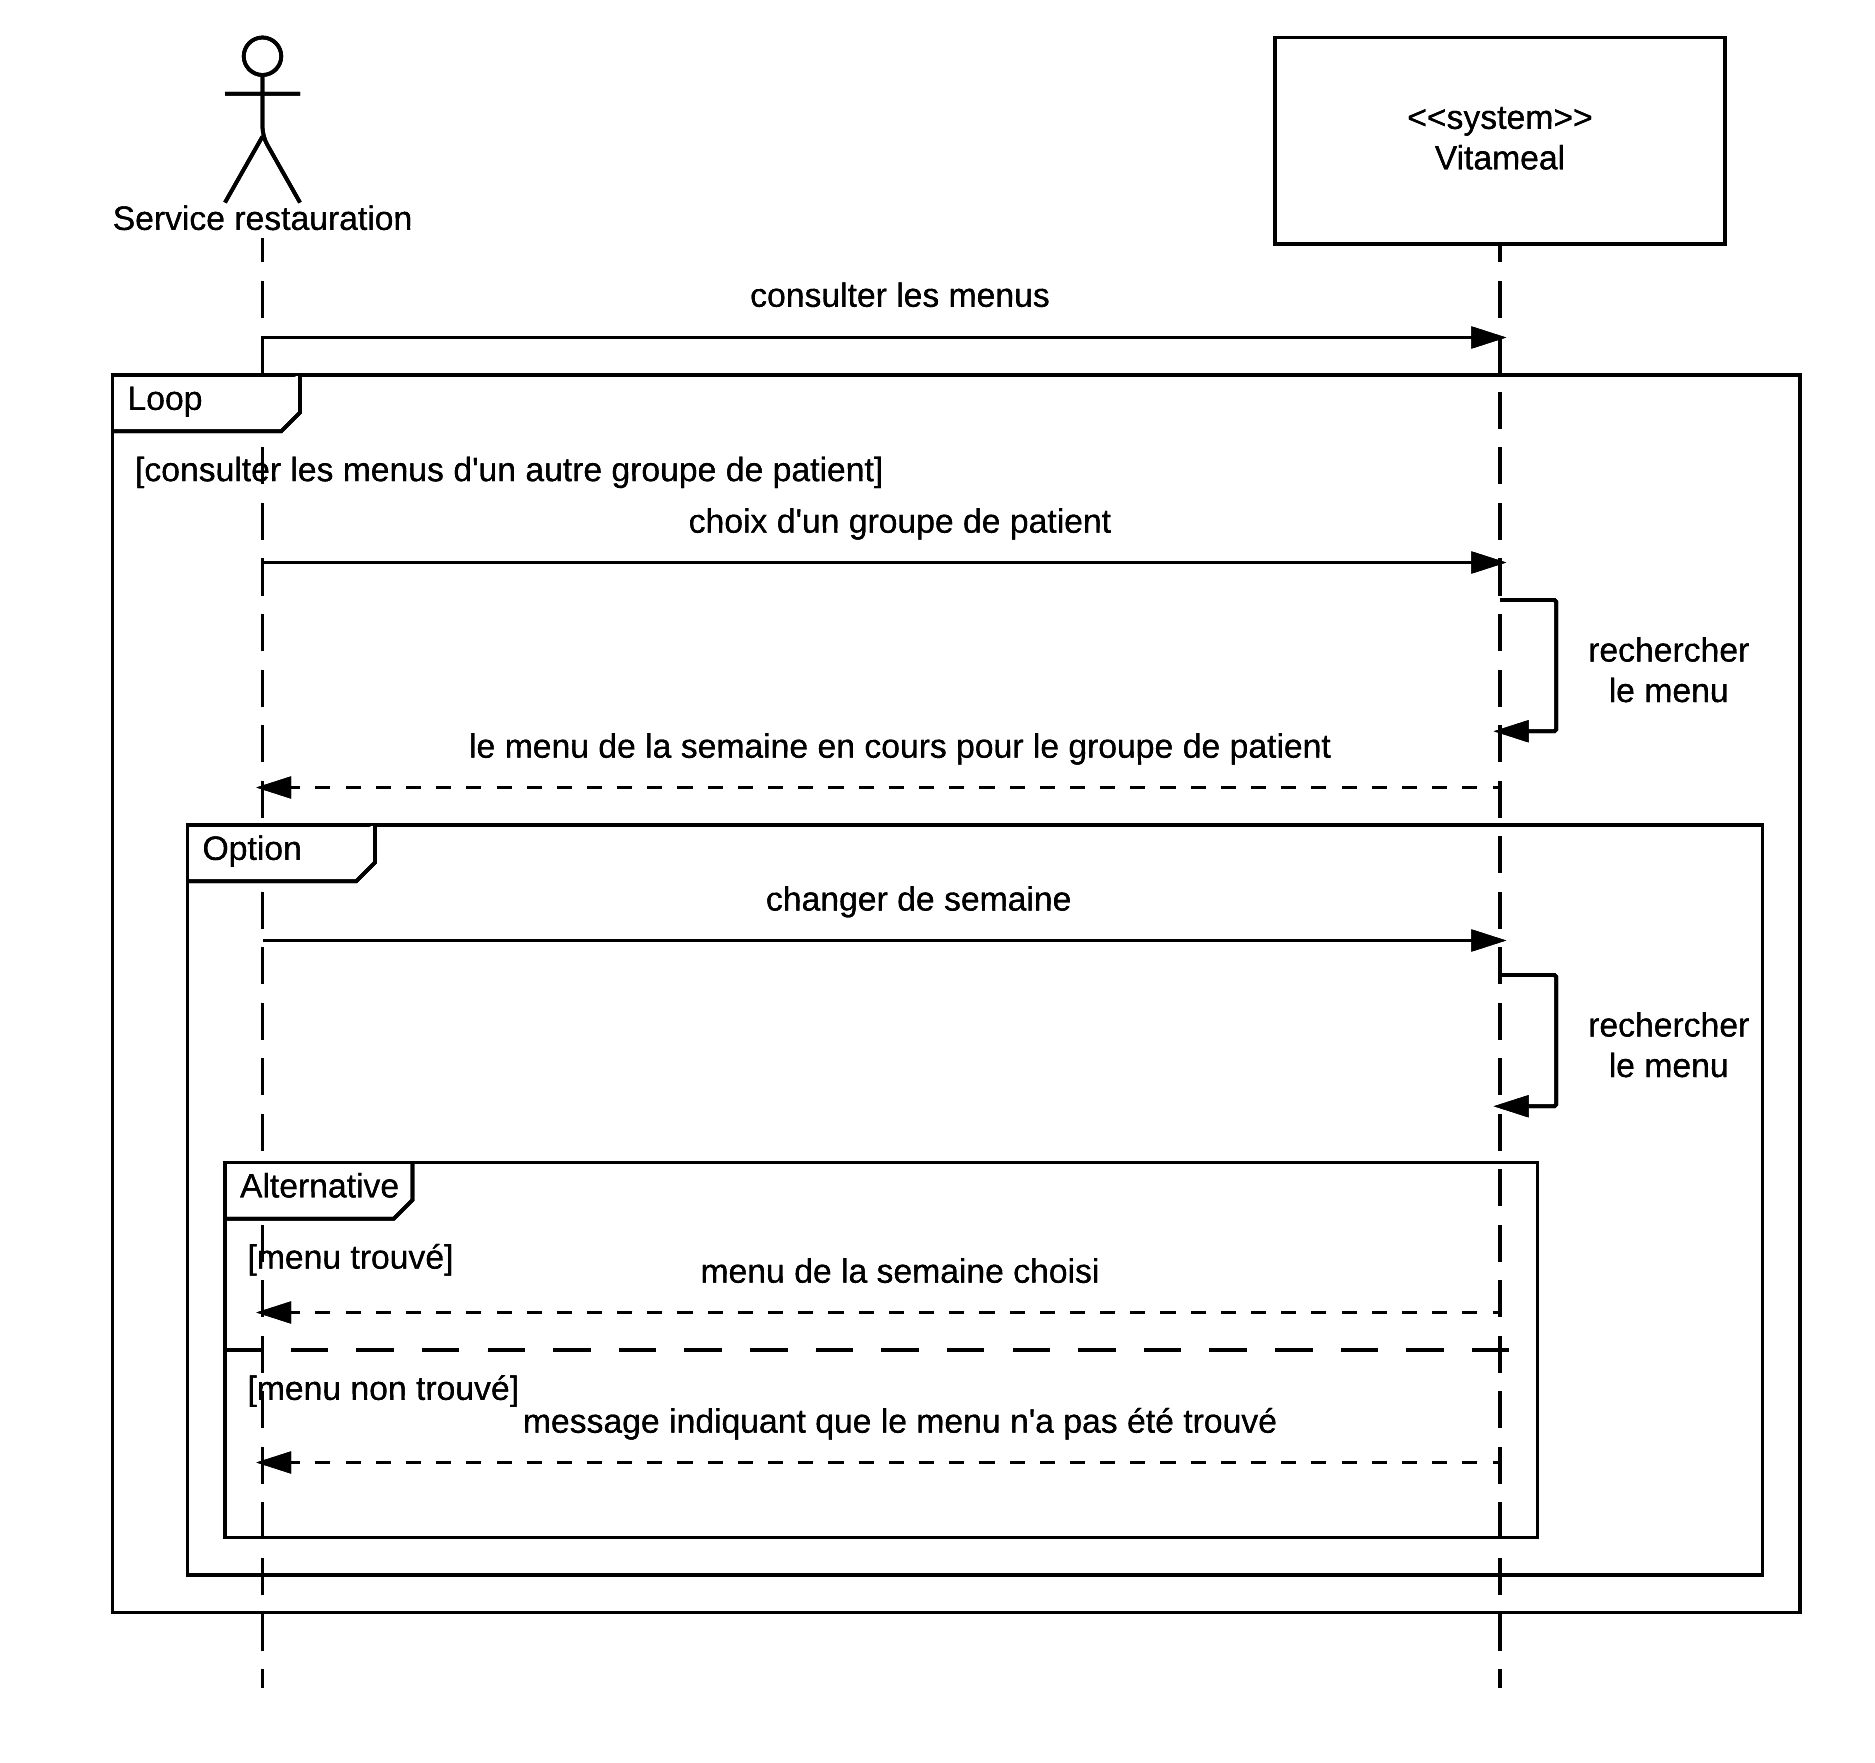
\includegraphics[scale=0.75]{../../CasDUtilisations/ConsulterMenus/sequence_consulter_menus.png}
\caption{Diagramme de séquence du cas d'utilisation consulter les menus}
\label{ConsulterMenusSeq}
\end{figure}

\subsubsection{Composer un plat}

\noindent \textbf{Nom:} Composer un plat \\
\textbf{ID:} UC401\\
\textbf{Description :} Le diététicien souhaite pouvoir composé un plat (petit-déjeuner, déjeuner, souper) en renseignant sa composition.\\
\textbf{Auteurs :} Nicolas SYMPHORIEN\\
\textbf{Date :} 16/06/2017 \\
\textbf{Acteurs :} Le diététicien \\
\textbf{Pré-condition :} \\
Le diététicien doit être connecter (Voir le cas d'utilisation secondaire ``S'authentifier''). \\
La liste des plats doit être accessible.

\noindent \textbf{Scénario principal : } Figure \ref{ComposerPlatSeq}

\begin{enumerate}
	\item \label{UC401_step1}Le système affiche la liste des plats déjà crée.
	\item \label{UC401_step2}Le diététicien choisi de créer un nouveau plat.
	\item Le système affiche une page permettant d'entrer les ingrédients composant le plat ainsi que leurs quantités
	\item Le diététicien choisi les ingrédients qu'il veut mettre dans son plat
	\item Le système enregistre le plat crée et affiche un message de confirmation de création
\end{enumerate}

 \noindent \textbf{Scénario alternatif :}

Les deux scénario alternatifs débute après l'étape \ref{UC401_step1} du scénario nominal.
\begin{enumerate}
	\item Le diététicien choisi de modifier un plat déjà existant.
	\begin{enumerate}
		\item Le système affiche les ingrédients du plat à modifier
		\item Le diététicien modifie la composition du plat et confirme les modifications
		\item Le système enregistre le plat modifié et affiche un message de confirmation de modification
	\end{enumerate}
	\item Le diététicien choisi de supprimer un plat déjà existant.
	\begin{enumerate}
		\item Le système affiche un message d'avertissement avant la suppression
		\item L'utilisateur confirme la suppression du plat
		\item Le système supprime le plat modifié et affiche un message de confirmation de suppression
	\end{enumerate}
\end{enumerate}
Dans les deux cas, le cas d'utilisation reprend à l'étape \ref{UC401_step2} du scénario nominal.

\noindent \textbf{Post-Conditions:} Le plat est crée, modifié ou supprimé.

\begin{figure}
\centering
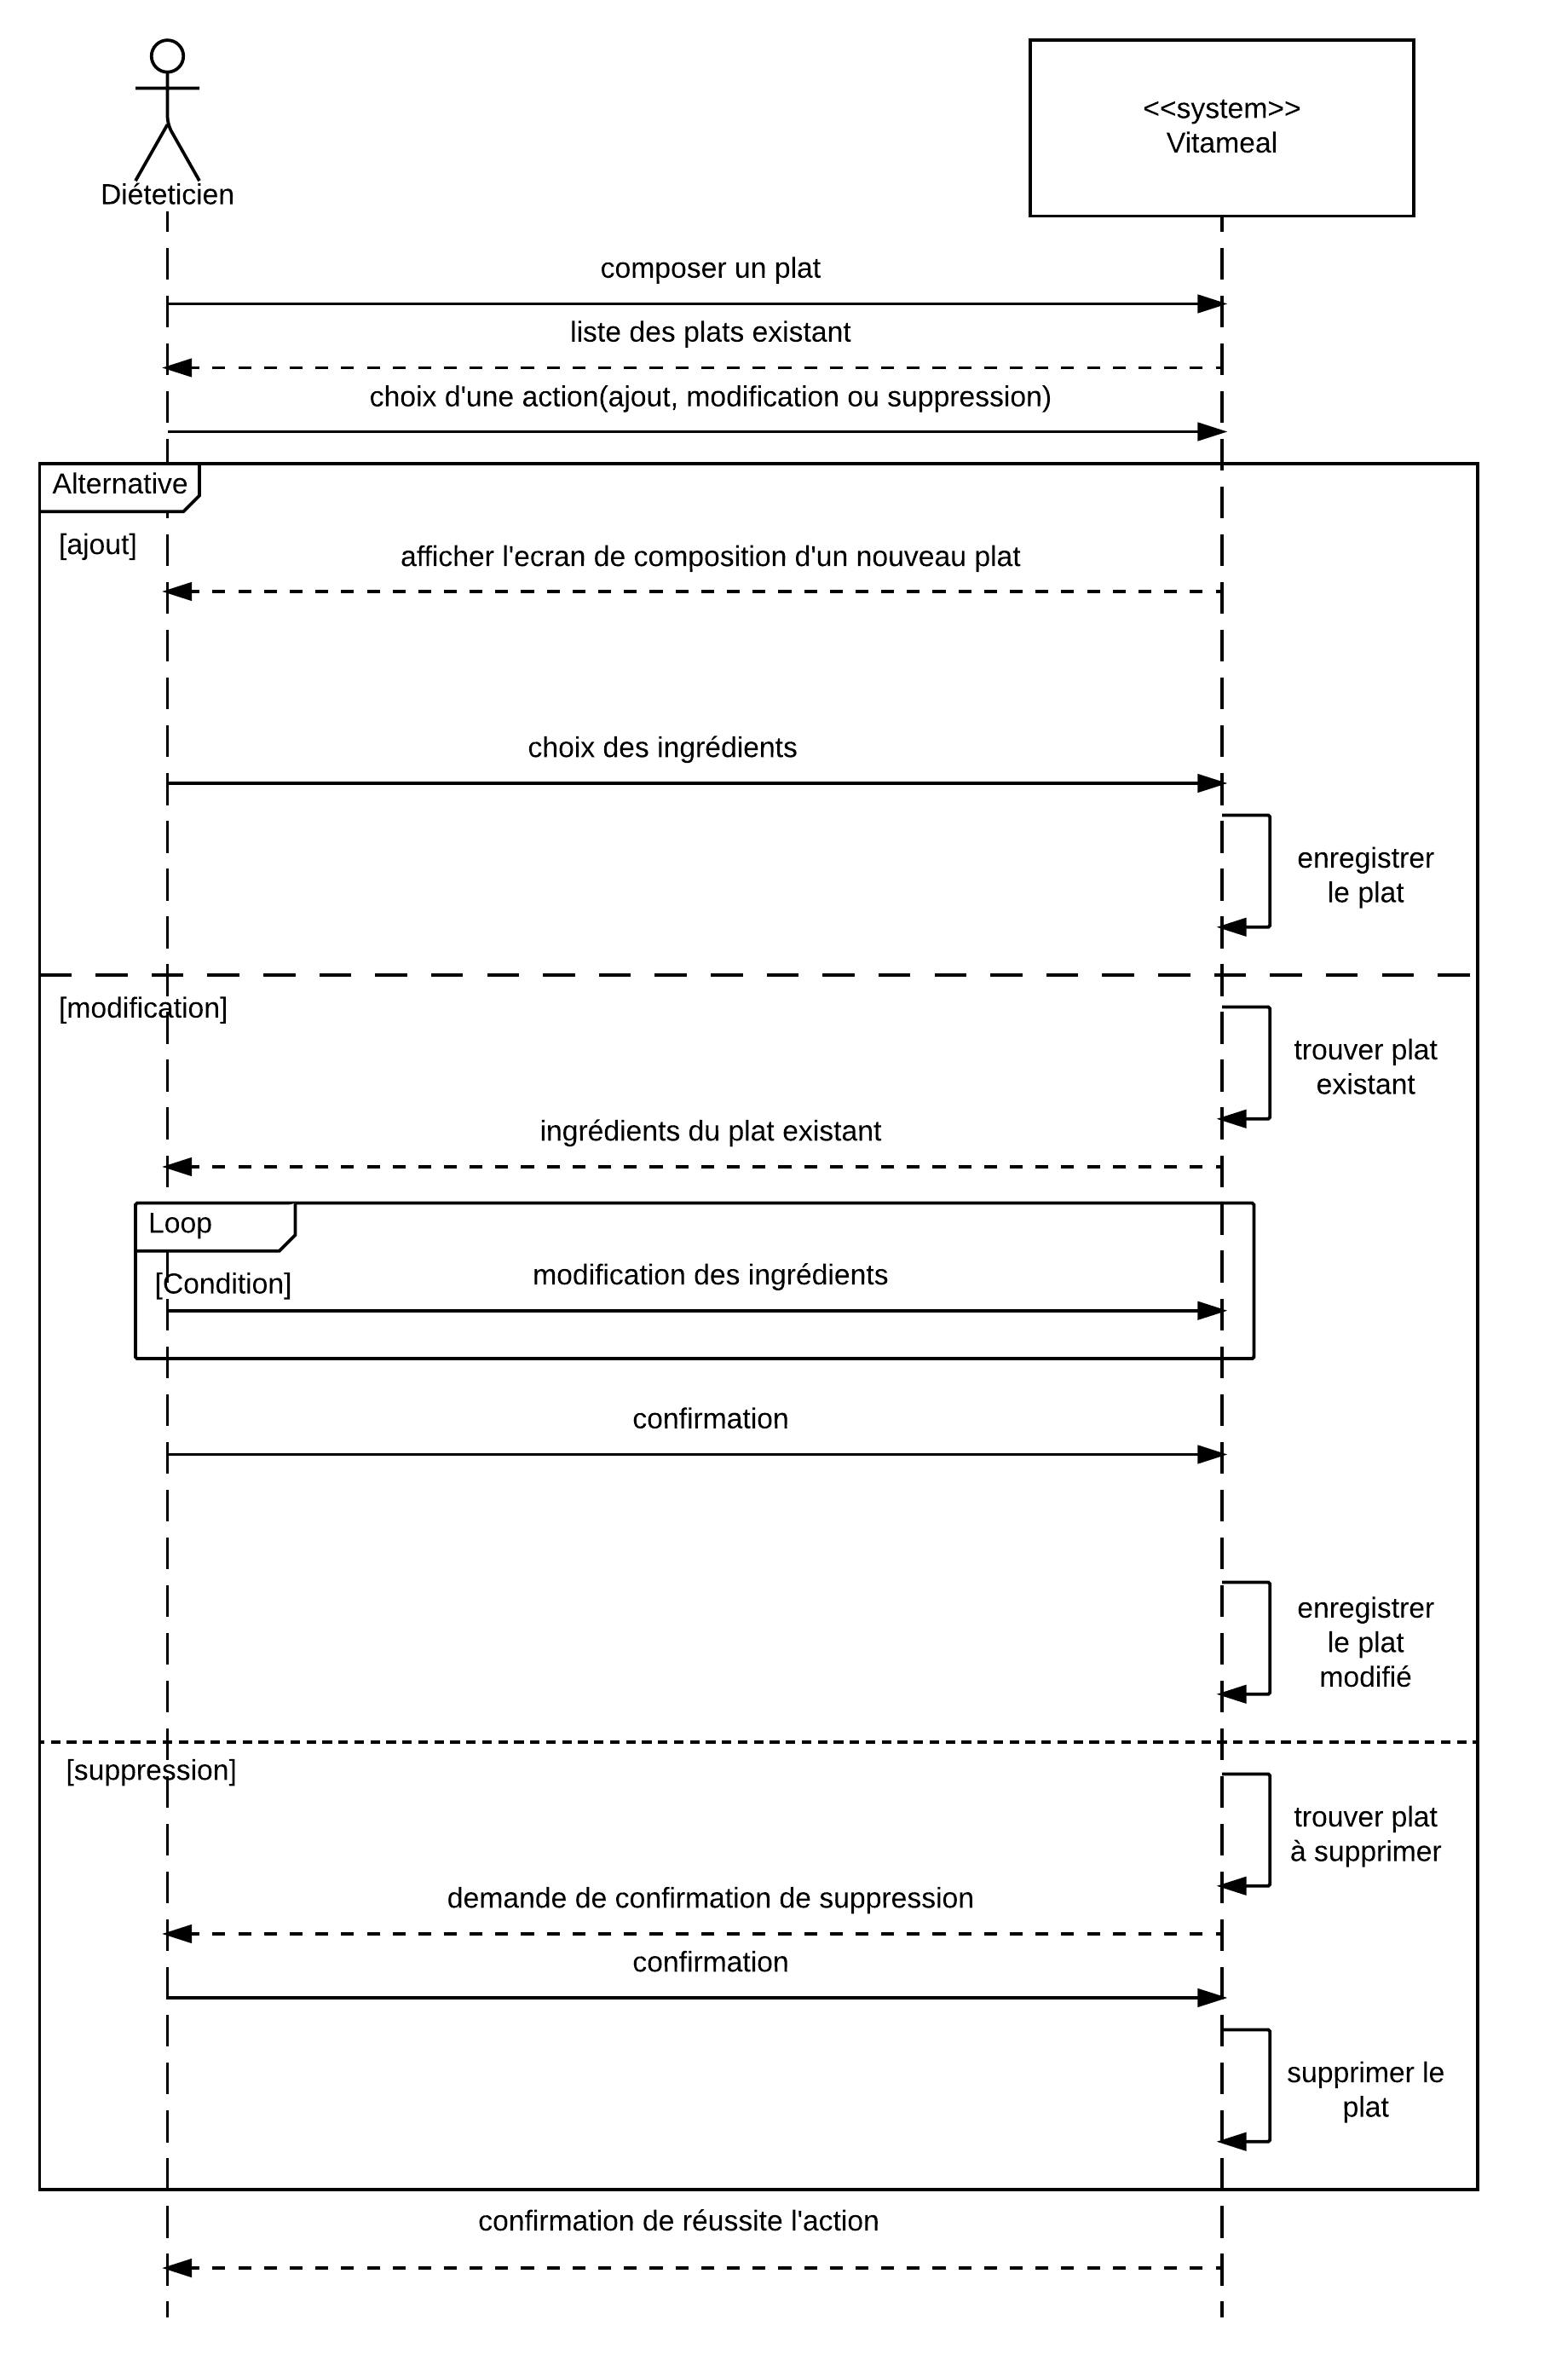
\includegraphics[scale=0.3]{../../CasDUtilisations/CompositionPlat/sequence_UC_ComposerPlat.png}
\caption{Diagramme de séquence du cas d'utilisation composer un plat}
\label{ComposerPlatSeq}
\end{figure}

\subsubsection{Composer un plat - conception détaillée}

L'analyse du cas d'utilisation composer un plat révèle quatre opérations : l'ajout, la modification, suppression et la consultation de plat. Se qui revient à définir les opérations CRUD (Create, Read, Delete, Update) pour la persistances des plats.

De plus, la solution doit respecter un modèle MVC.

Pour le modèle, les plats sont représenter par trois entités JPA : Plat, ComposantPlat, Ingrédient gérer par le framework Hibernate.L'entité ComposantPlat correspond à l'association d'un plat et d'un ingrédient et permet de stocker des informations comme la quantité d'un ingrédient dans un plat. De plus, chaque entité est géré par un DAO qui implémente les opérations CRUD.

Pour le contrôle, l'application utilise un servlet PlatServlet et un beans de contrôle PlatControleur.
La servlet est en charge de traiter les requête http GET et POST. Les requétes GET servent à envoyer le type d'opération à effectuer selon le format : /Plats\? action=[opération]\& id=[id du plat sur lequel porte l'action]. L'opération créer ne demande pas d'id, l'opération consulter sans id, revient à consulter tous les plats.
Les requêtes POST servent à envoyer les données servant à la création et à l'édition par le récupération des informations sur le plat dans un formulaire.
Le contrôleur traite les informations transmise à la servlet et modifie les entités selon l'opération demandé, elle a un durée de vie de type session et crée les DAO associé au entité.

La servlet redirige sur deux vue selon le type d'opération : consulterPlat.jsp pour les opérations consulter et supprimer, et editerPlat.jsp pour la création et l'édition. Chaque vue adapte son affichage en fonction du type d'opération. 

\begin{figure}
\centering
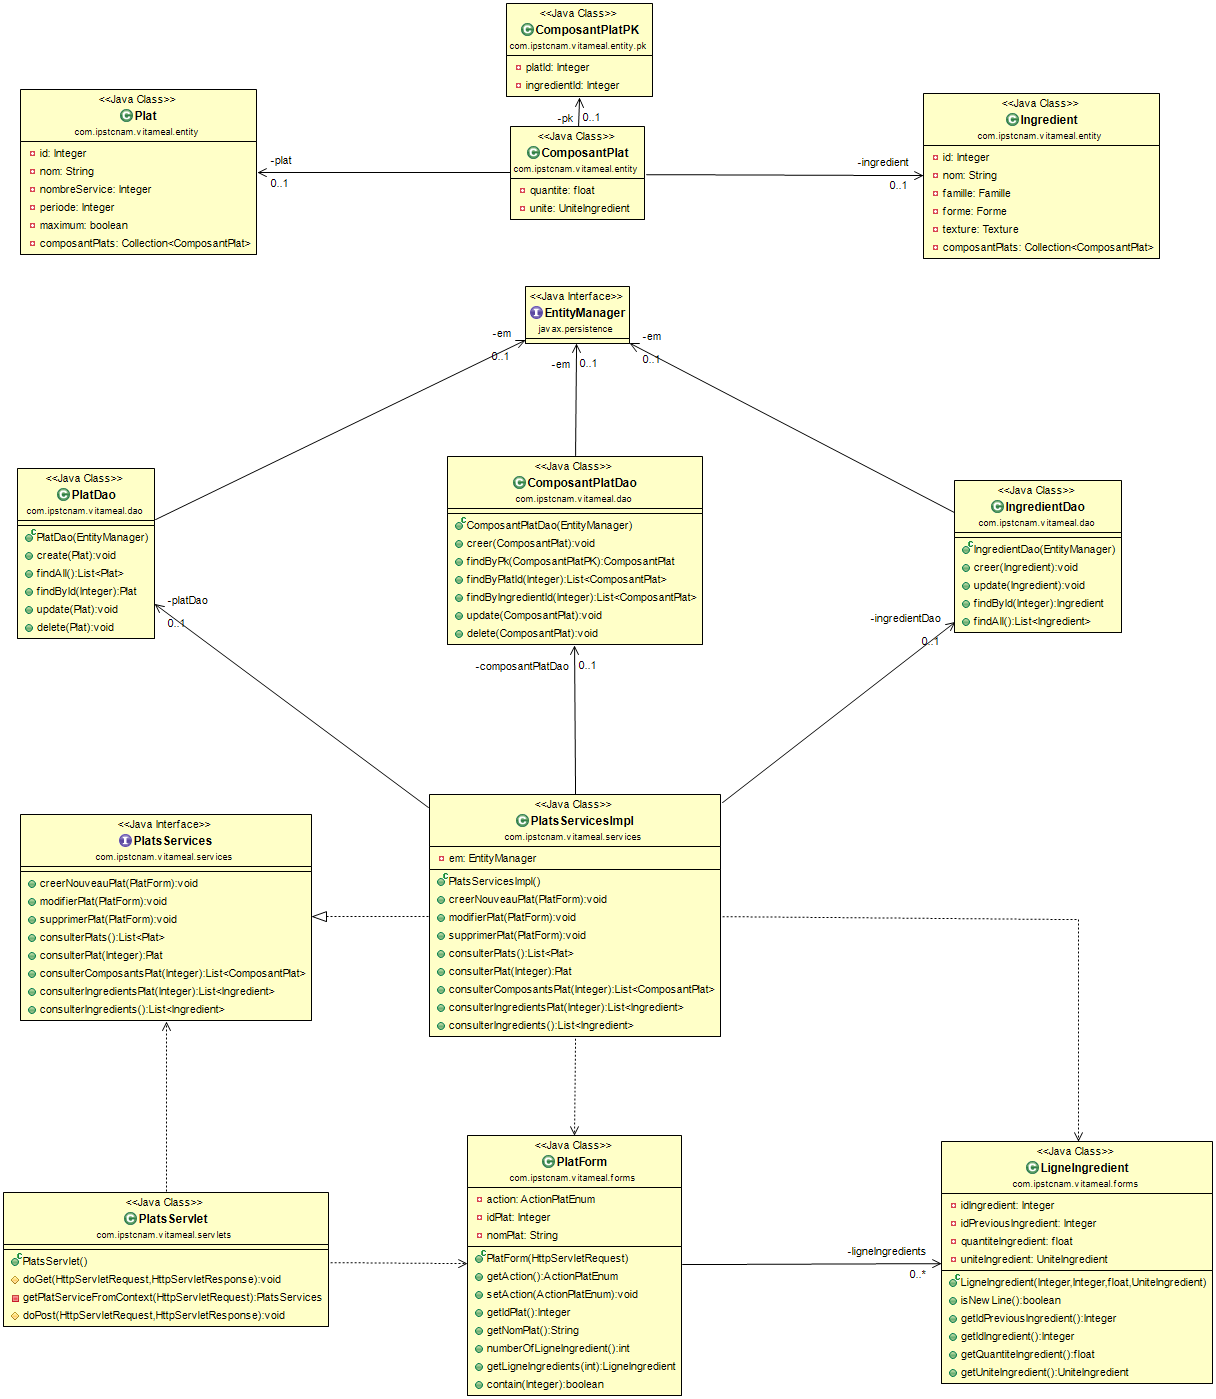
\includegraphics[scale=0.4]{../../CasDUtilisations/CompositionPlat/classDiagram_ComposerPlat.png}
\caption{Diagramme de classe de la compostion d'un plat}
\label{DiagrammeClassComposerPlat}
\end{figure}

\begin{figure}
\centering
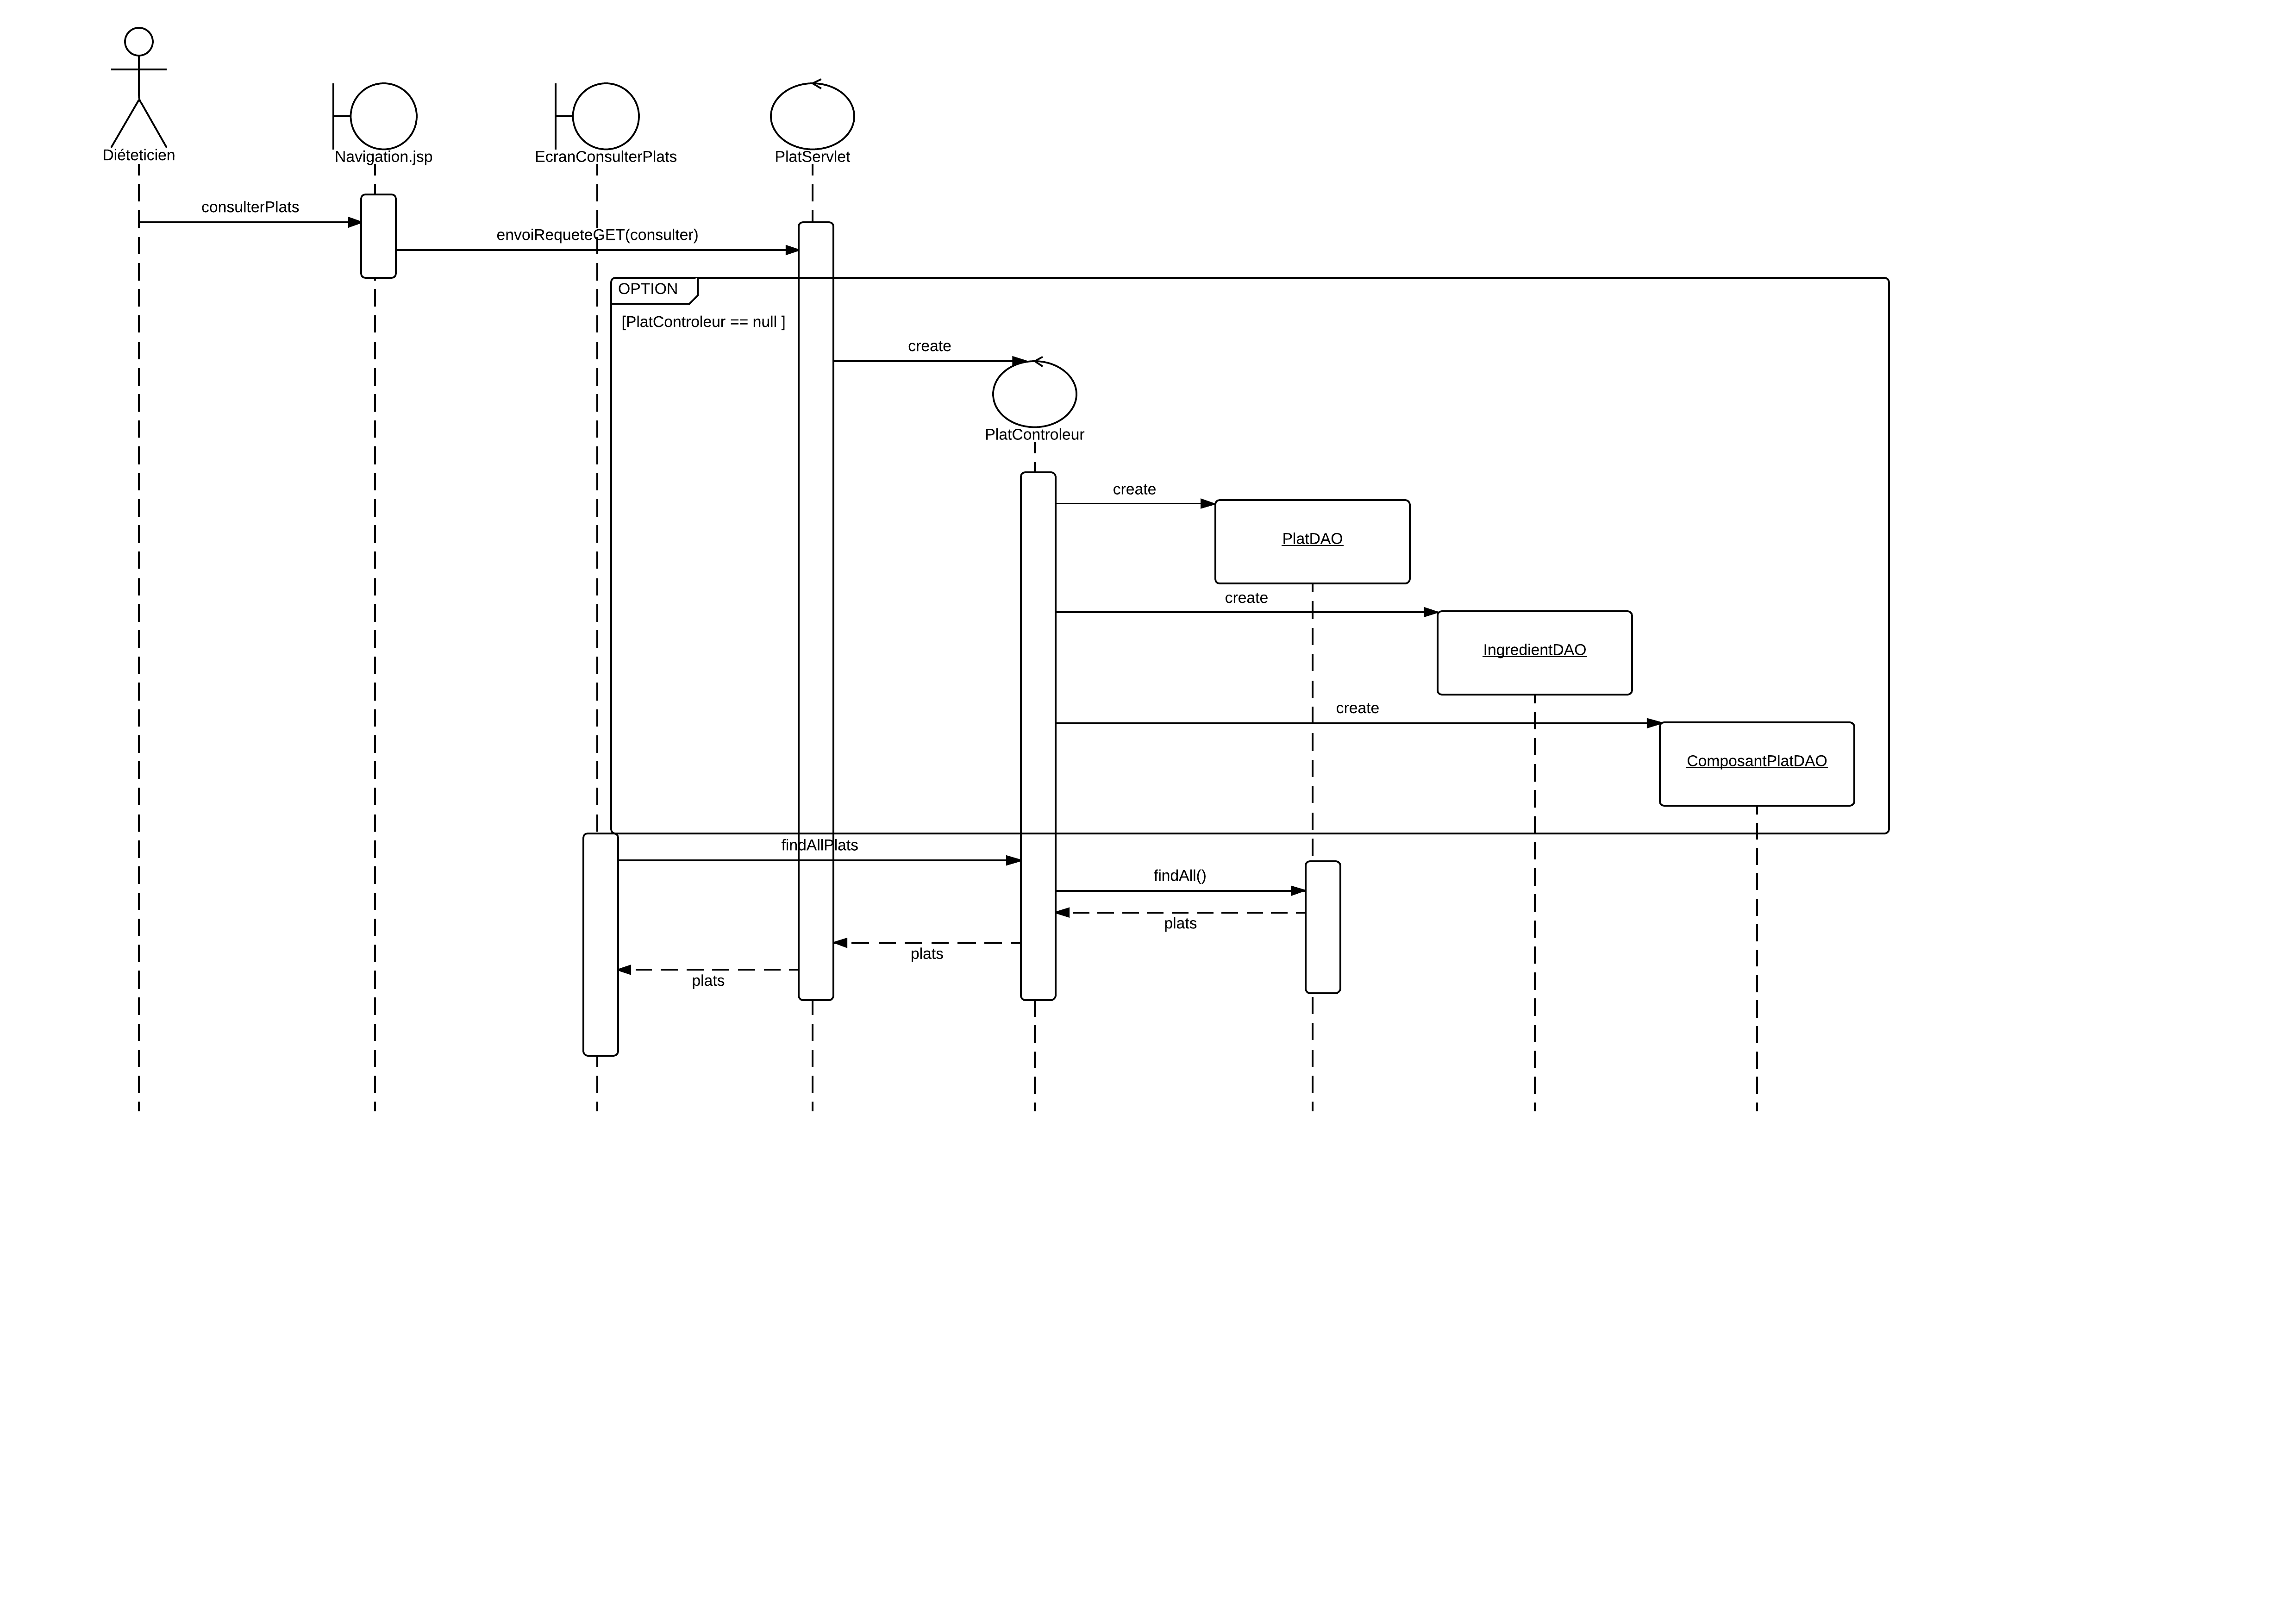
\includegraphics[scale=0.15]{../../CasDUtilisations/CompositionPlat/sequence_InitialisationPlatControleur.png}
\caption{Diagramme de séquence d'initialisation du contrôleur de plat}
\label{SequenceInitPlatControleur}
\end{figure}

\begin{figure}
\centering
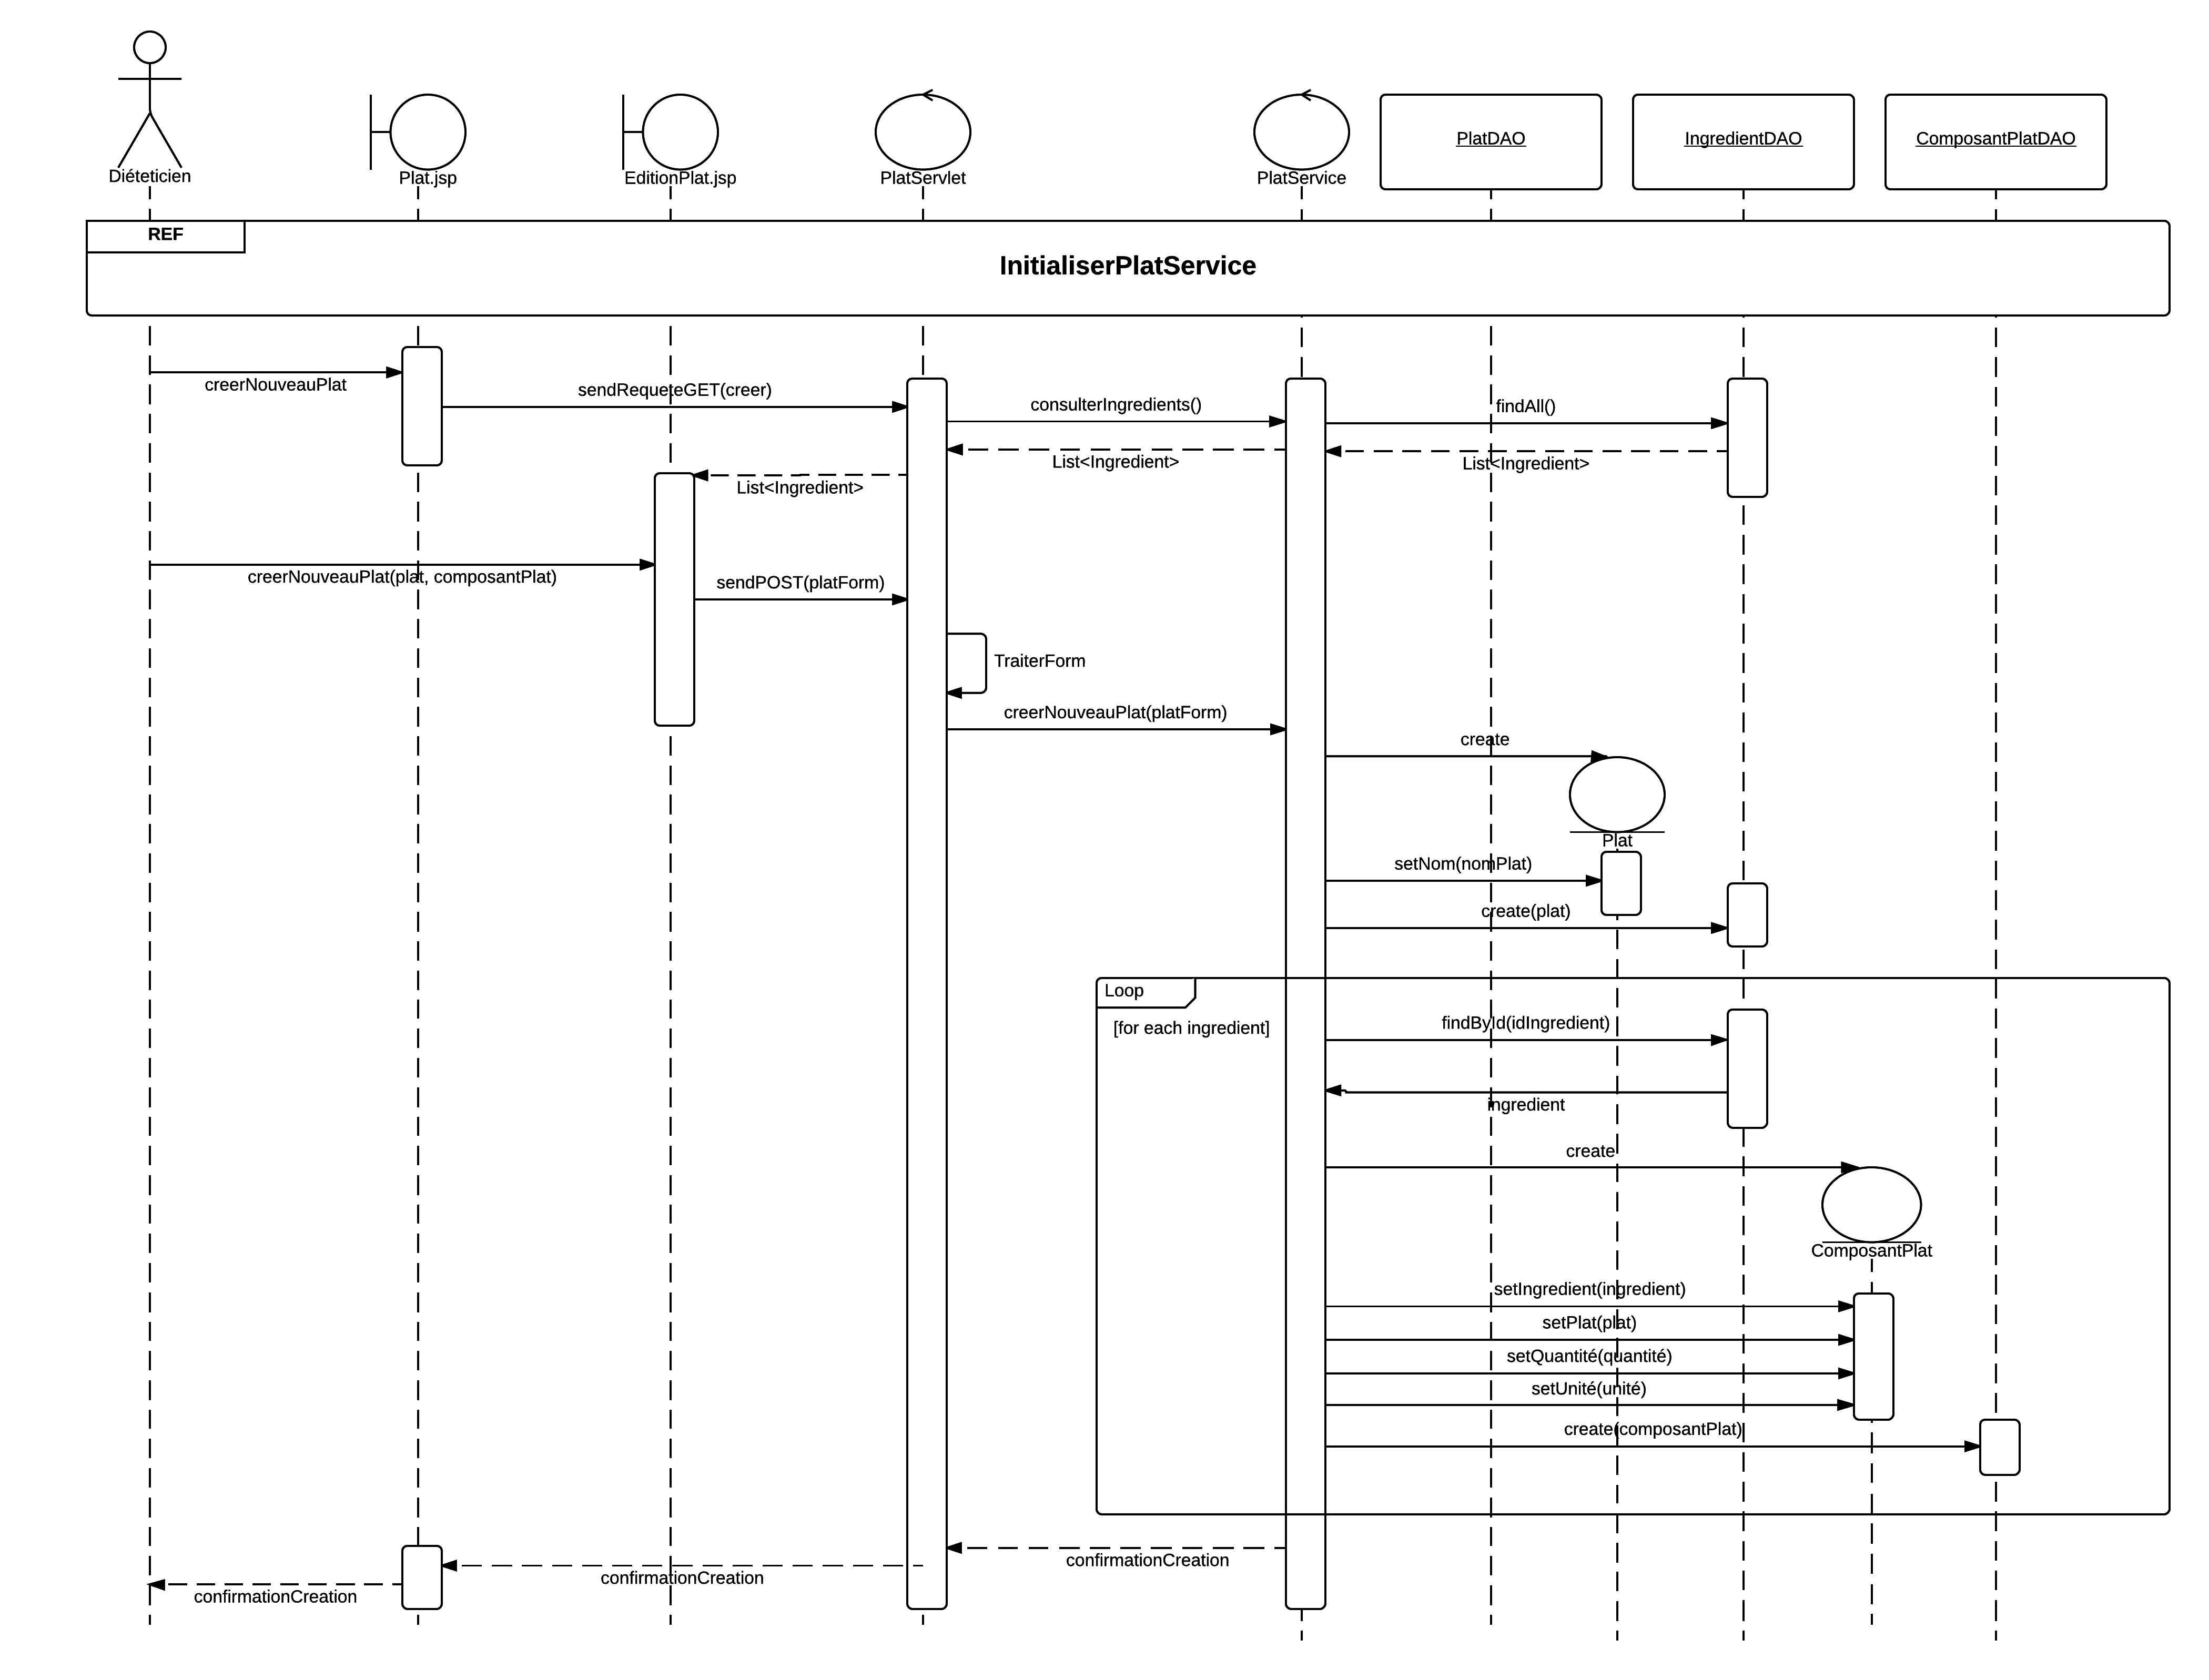
\includegraphics[scale=0.45]{../../CasDUtilisations/CompositionPlat/sequence_CreerPlat.png}
\caption{Diagramme de séquence de création d'un plat}
\label{SequenceCreerPlat}
\end{figure}

\begin{figure}
\centering
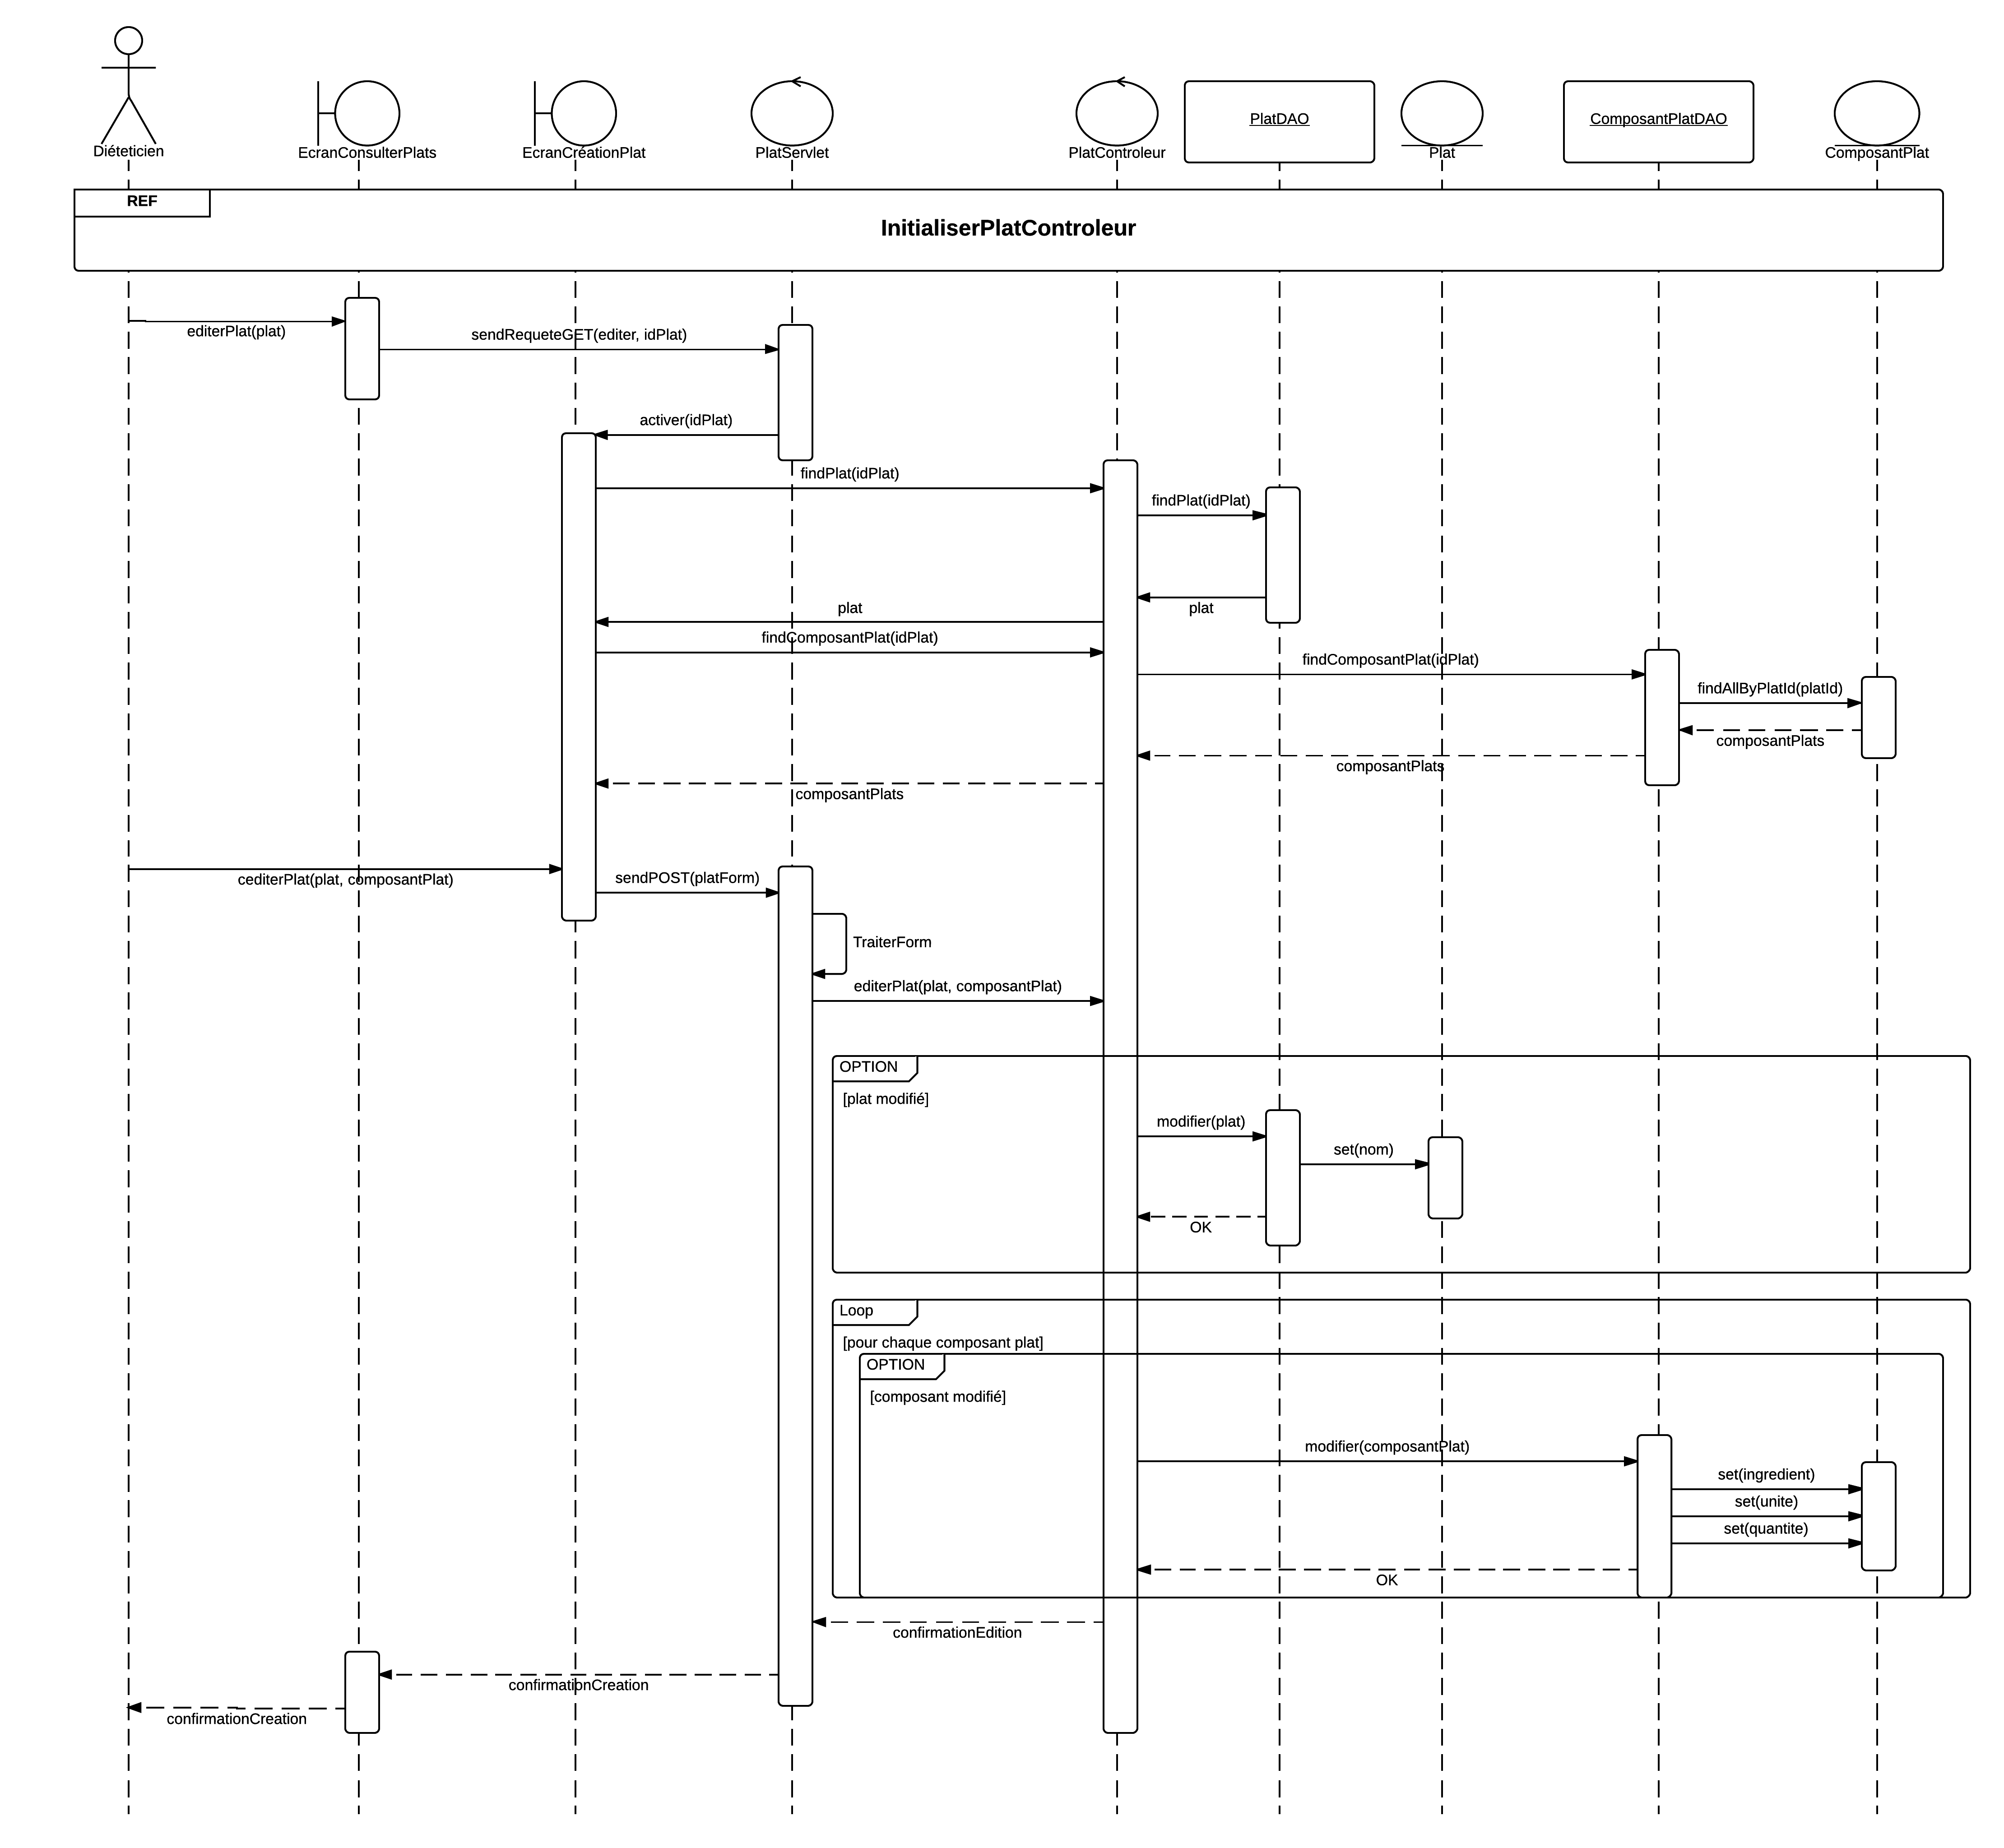
\includegraphics[scale=0.45]{../../CasDUtilisations/CompositionPlat/sequence_EditerPlat.png}
\caption{Diagramme de séquence d'édition d'un plat}
\label{SequenceEditerPlat}
\end{figure}

\begin{figure}
\centering
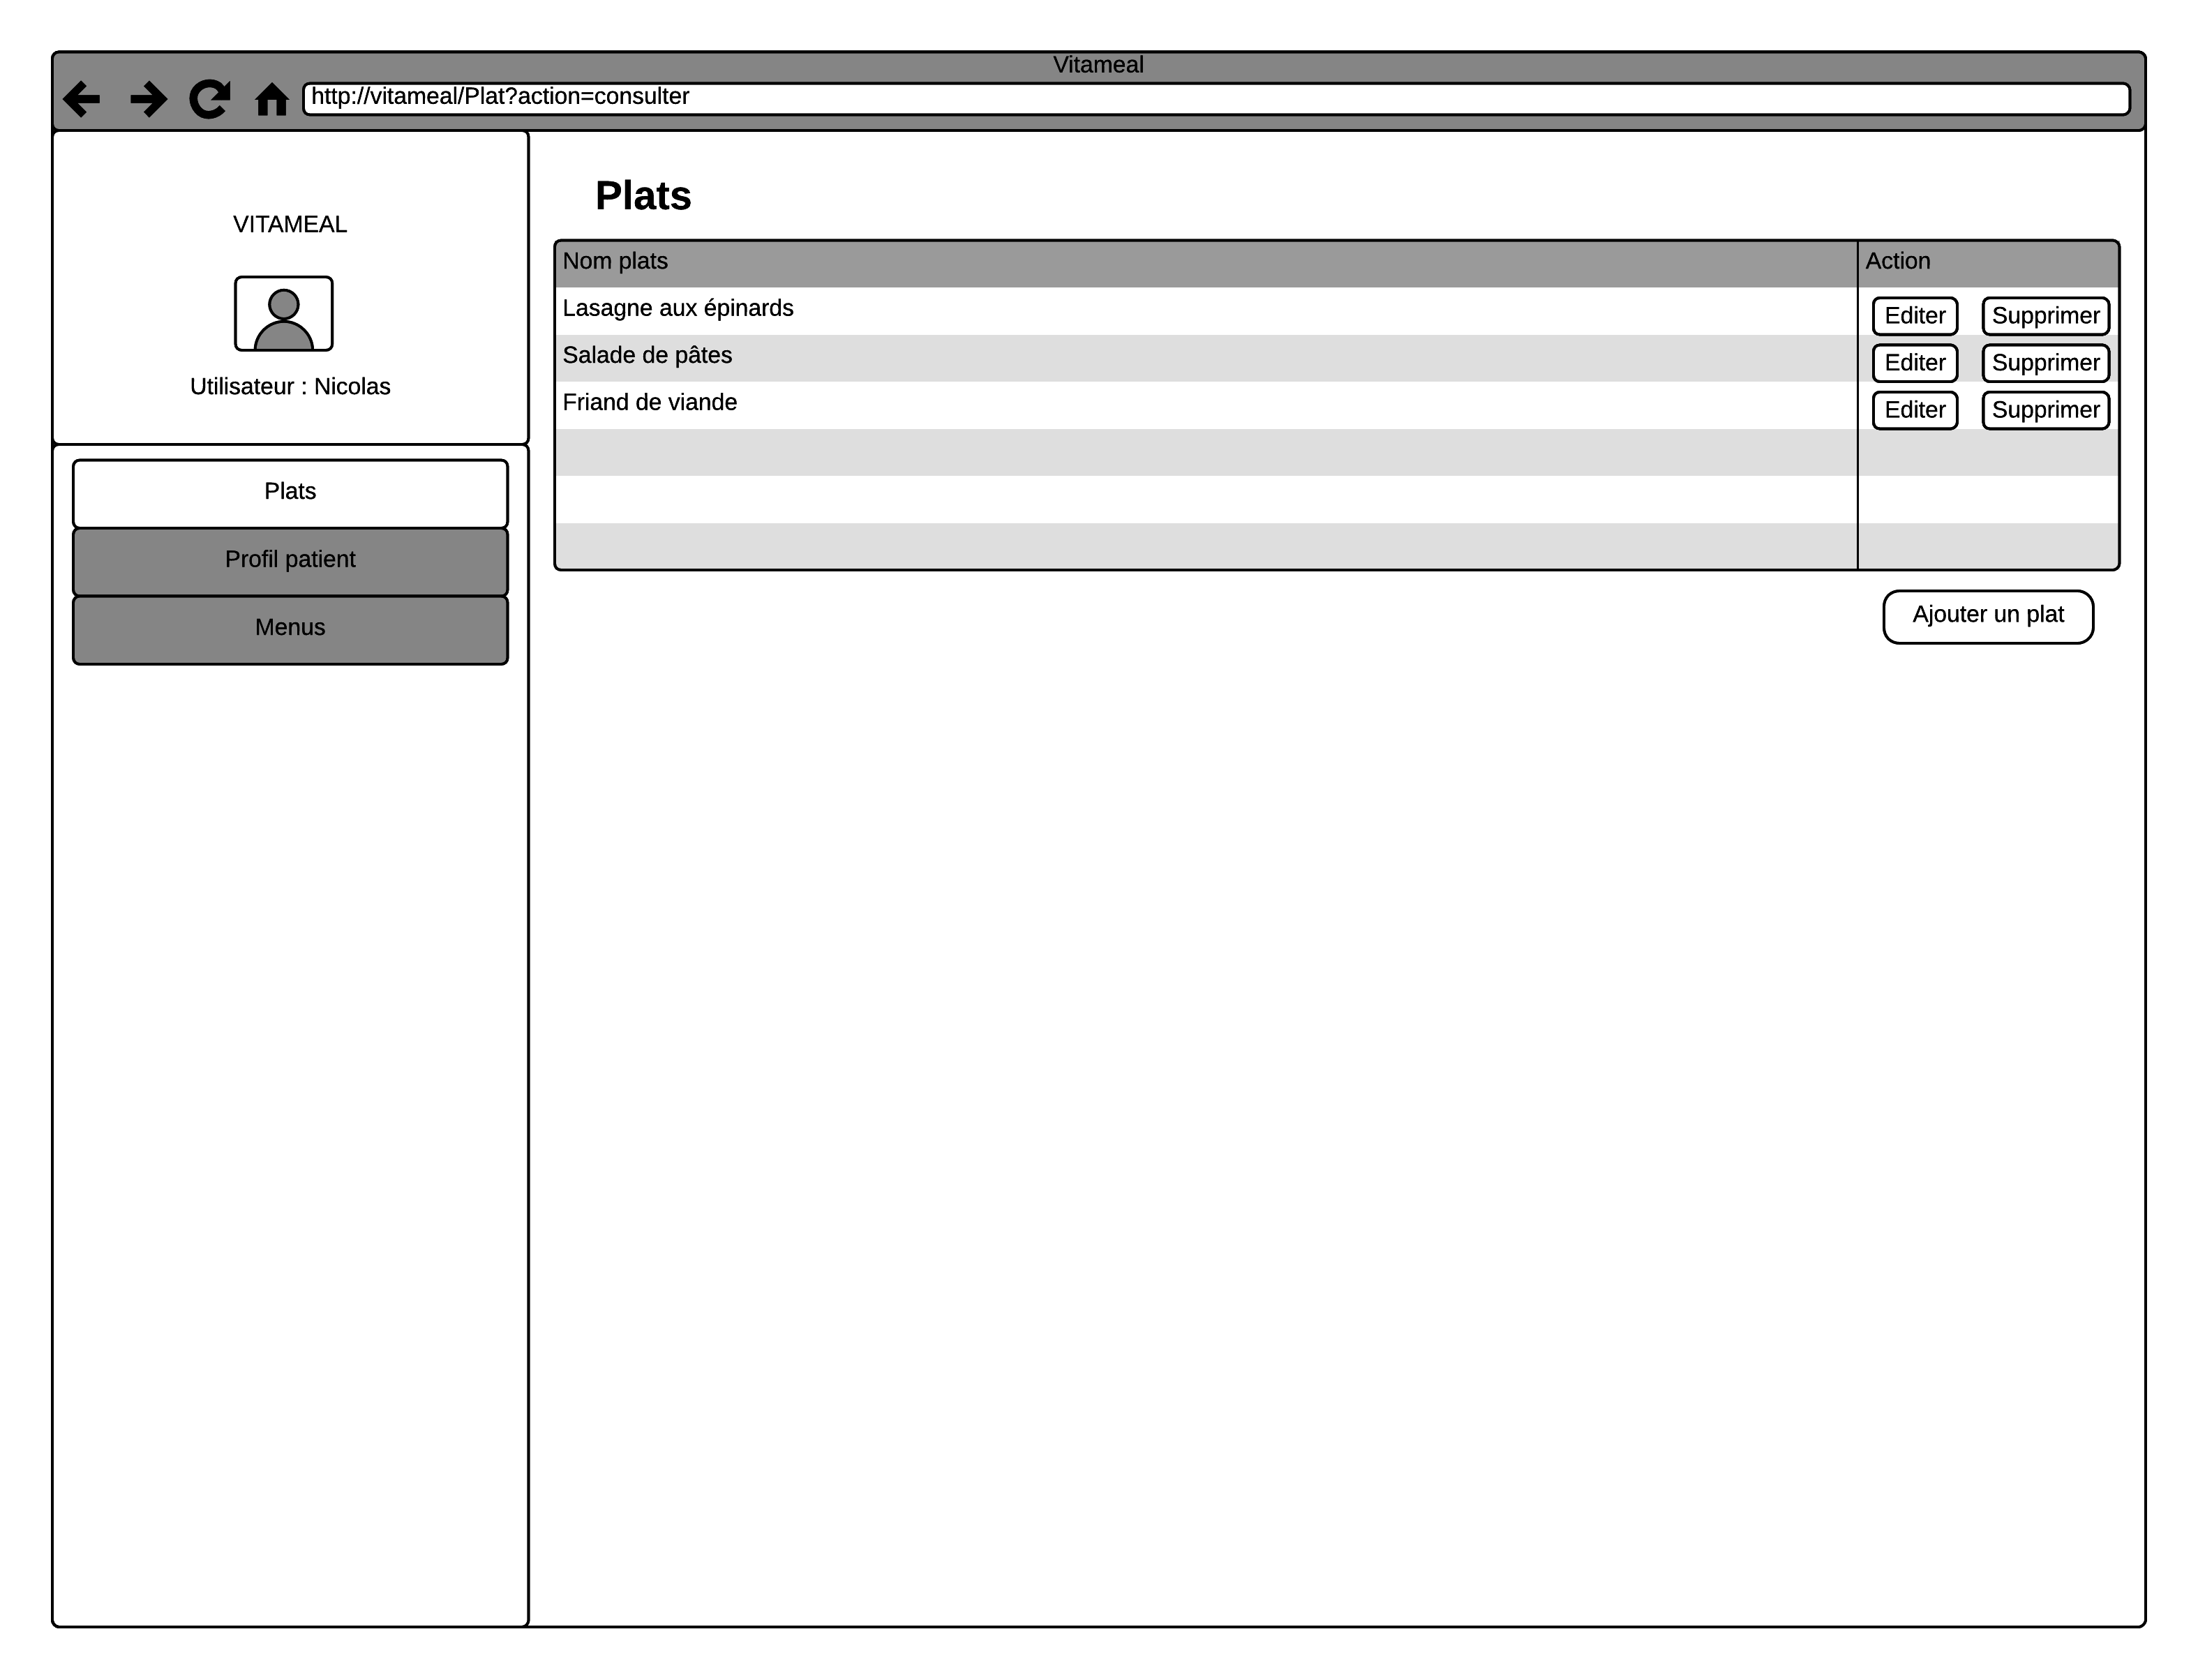
\includegraphics[scale=0.5]{../../CasDUtilisations/CompositionPlat/maquette_EcranConsulterPlats.png}
\caption{Maquette de consultation d'un plat}
\label{MaquetteConsultationPlat}
\end{figure}

\begin{figure}
\centering
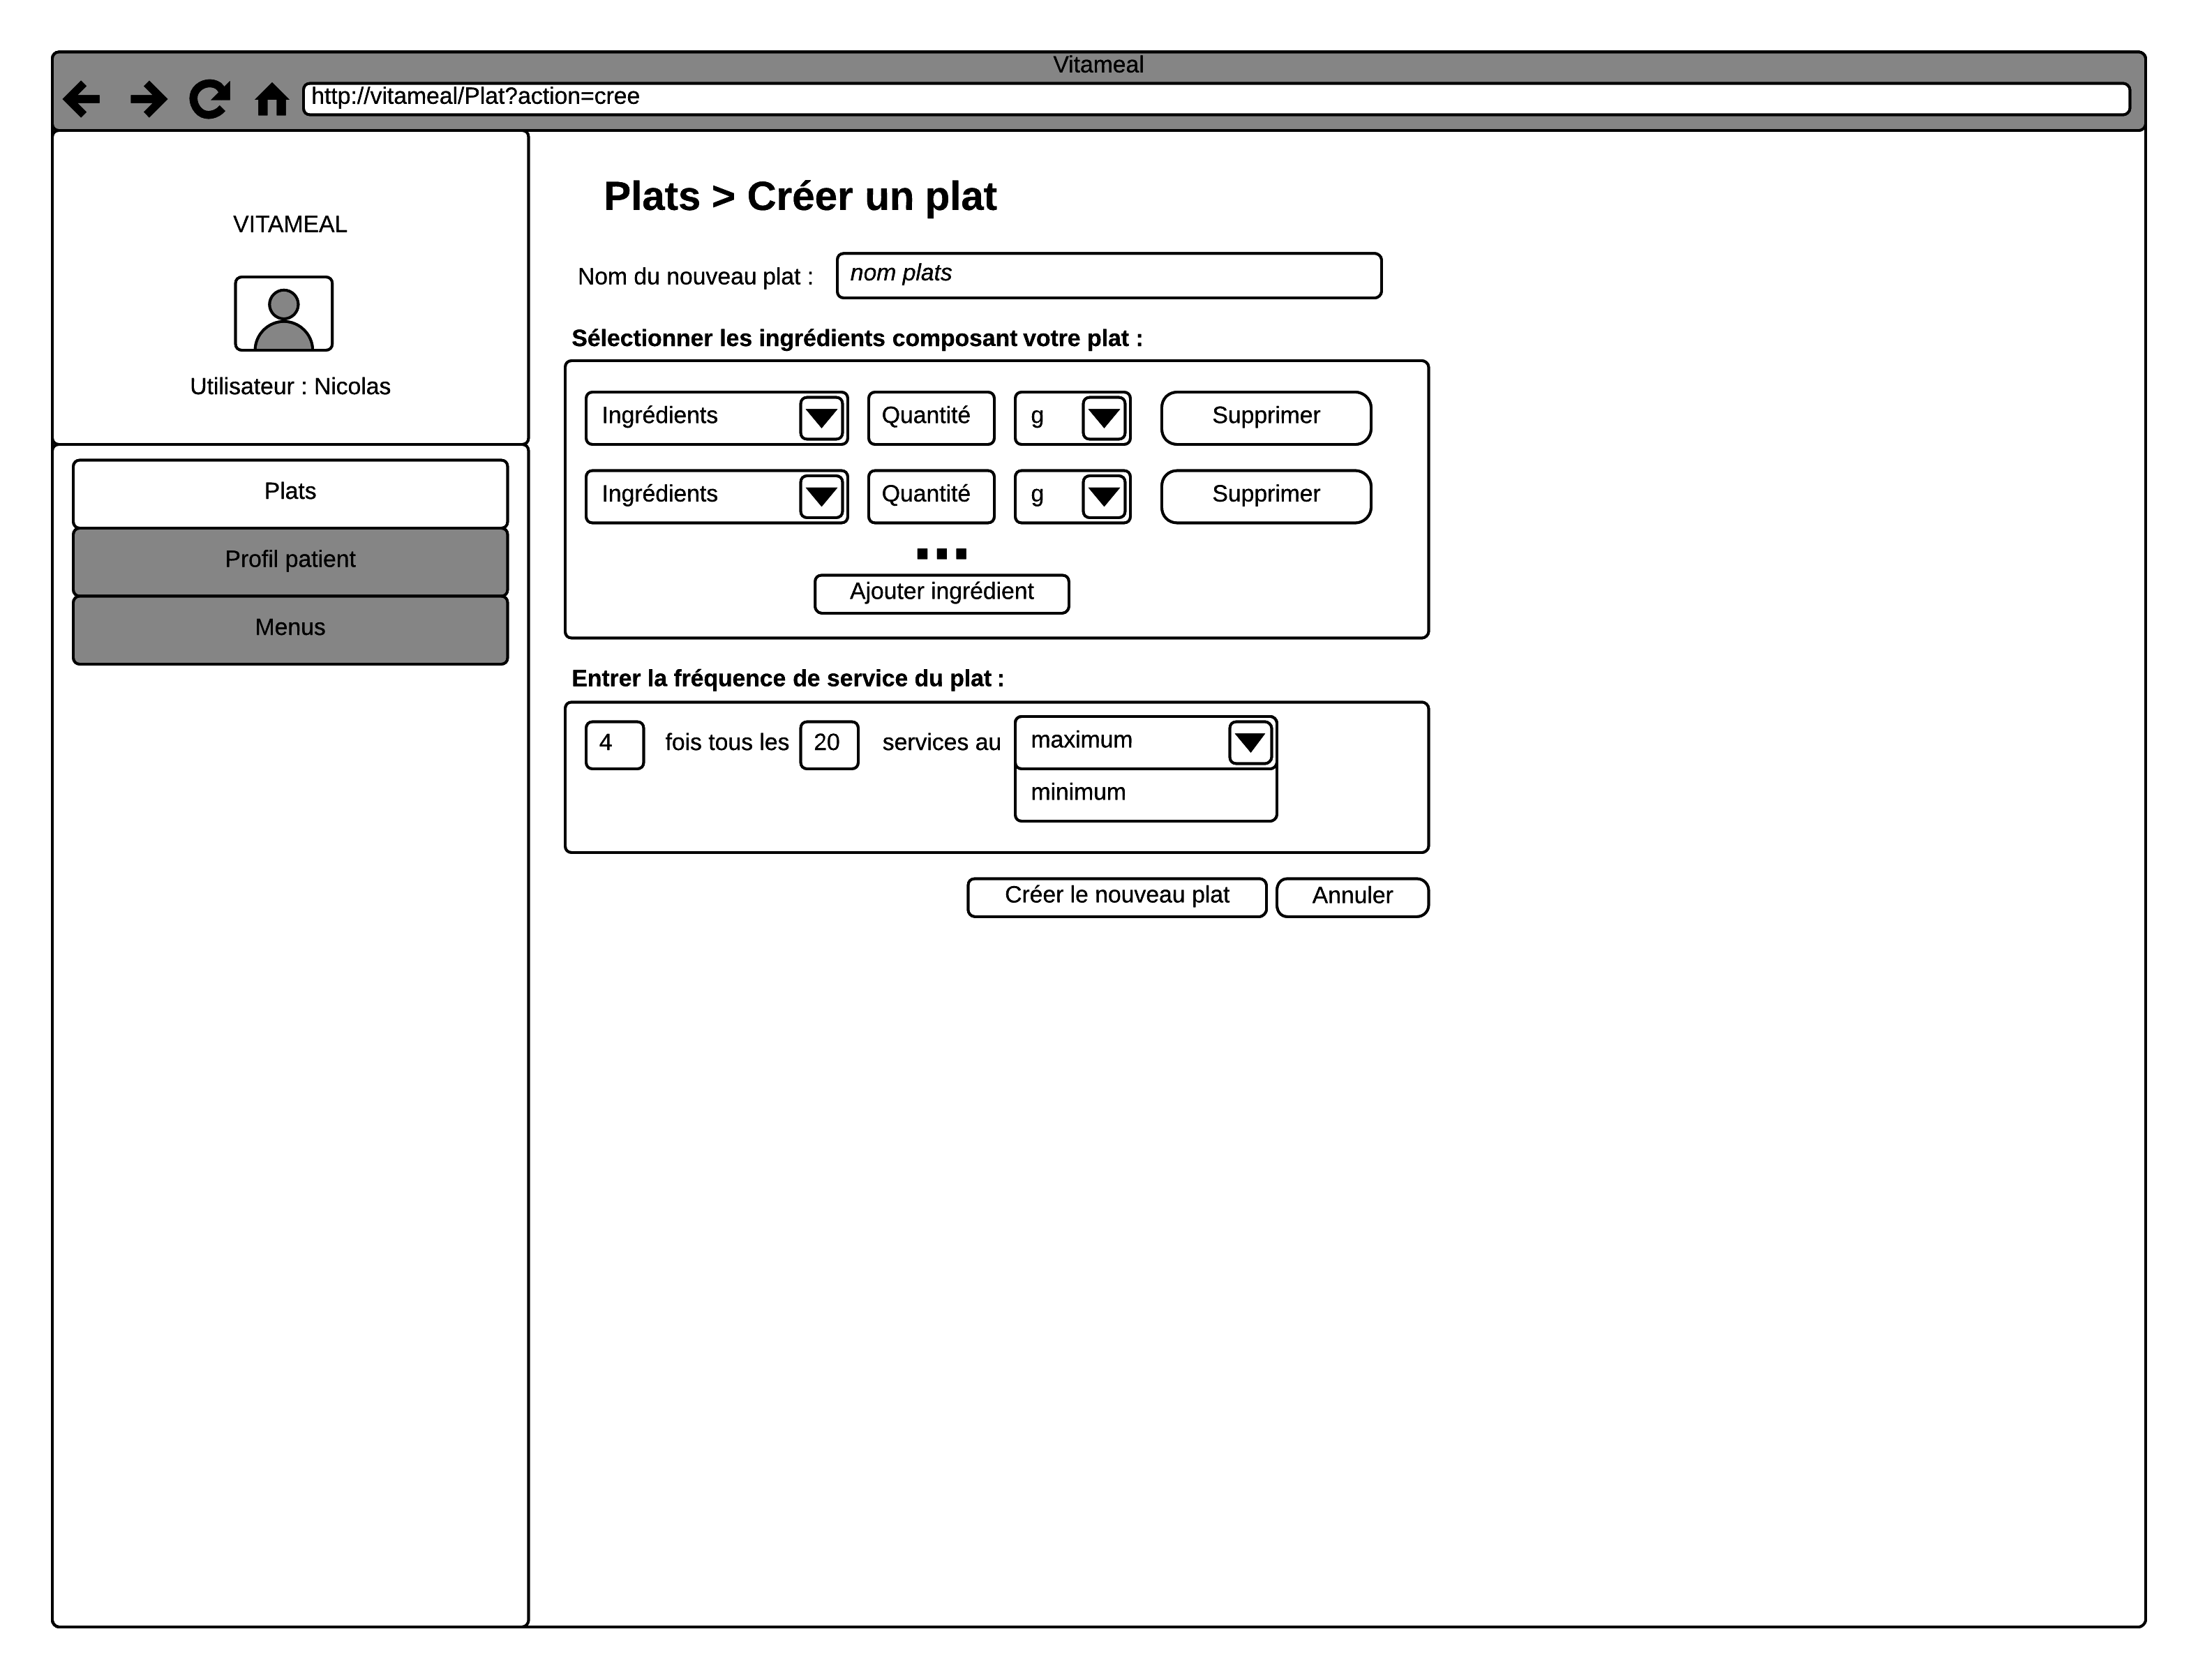
\includegraphics[scale=0.5]{../../CasDUtilisations/CompositionPlat/maquette_EcranCreationPlat.png}
\caption{Maquette de la création d'un plat}
\label{MaquetteCreationPlat}
\end{figure}

\begin{figure}
\centering
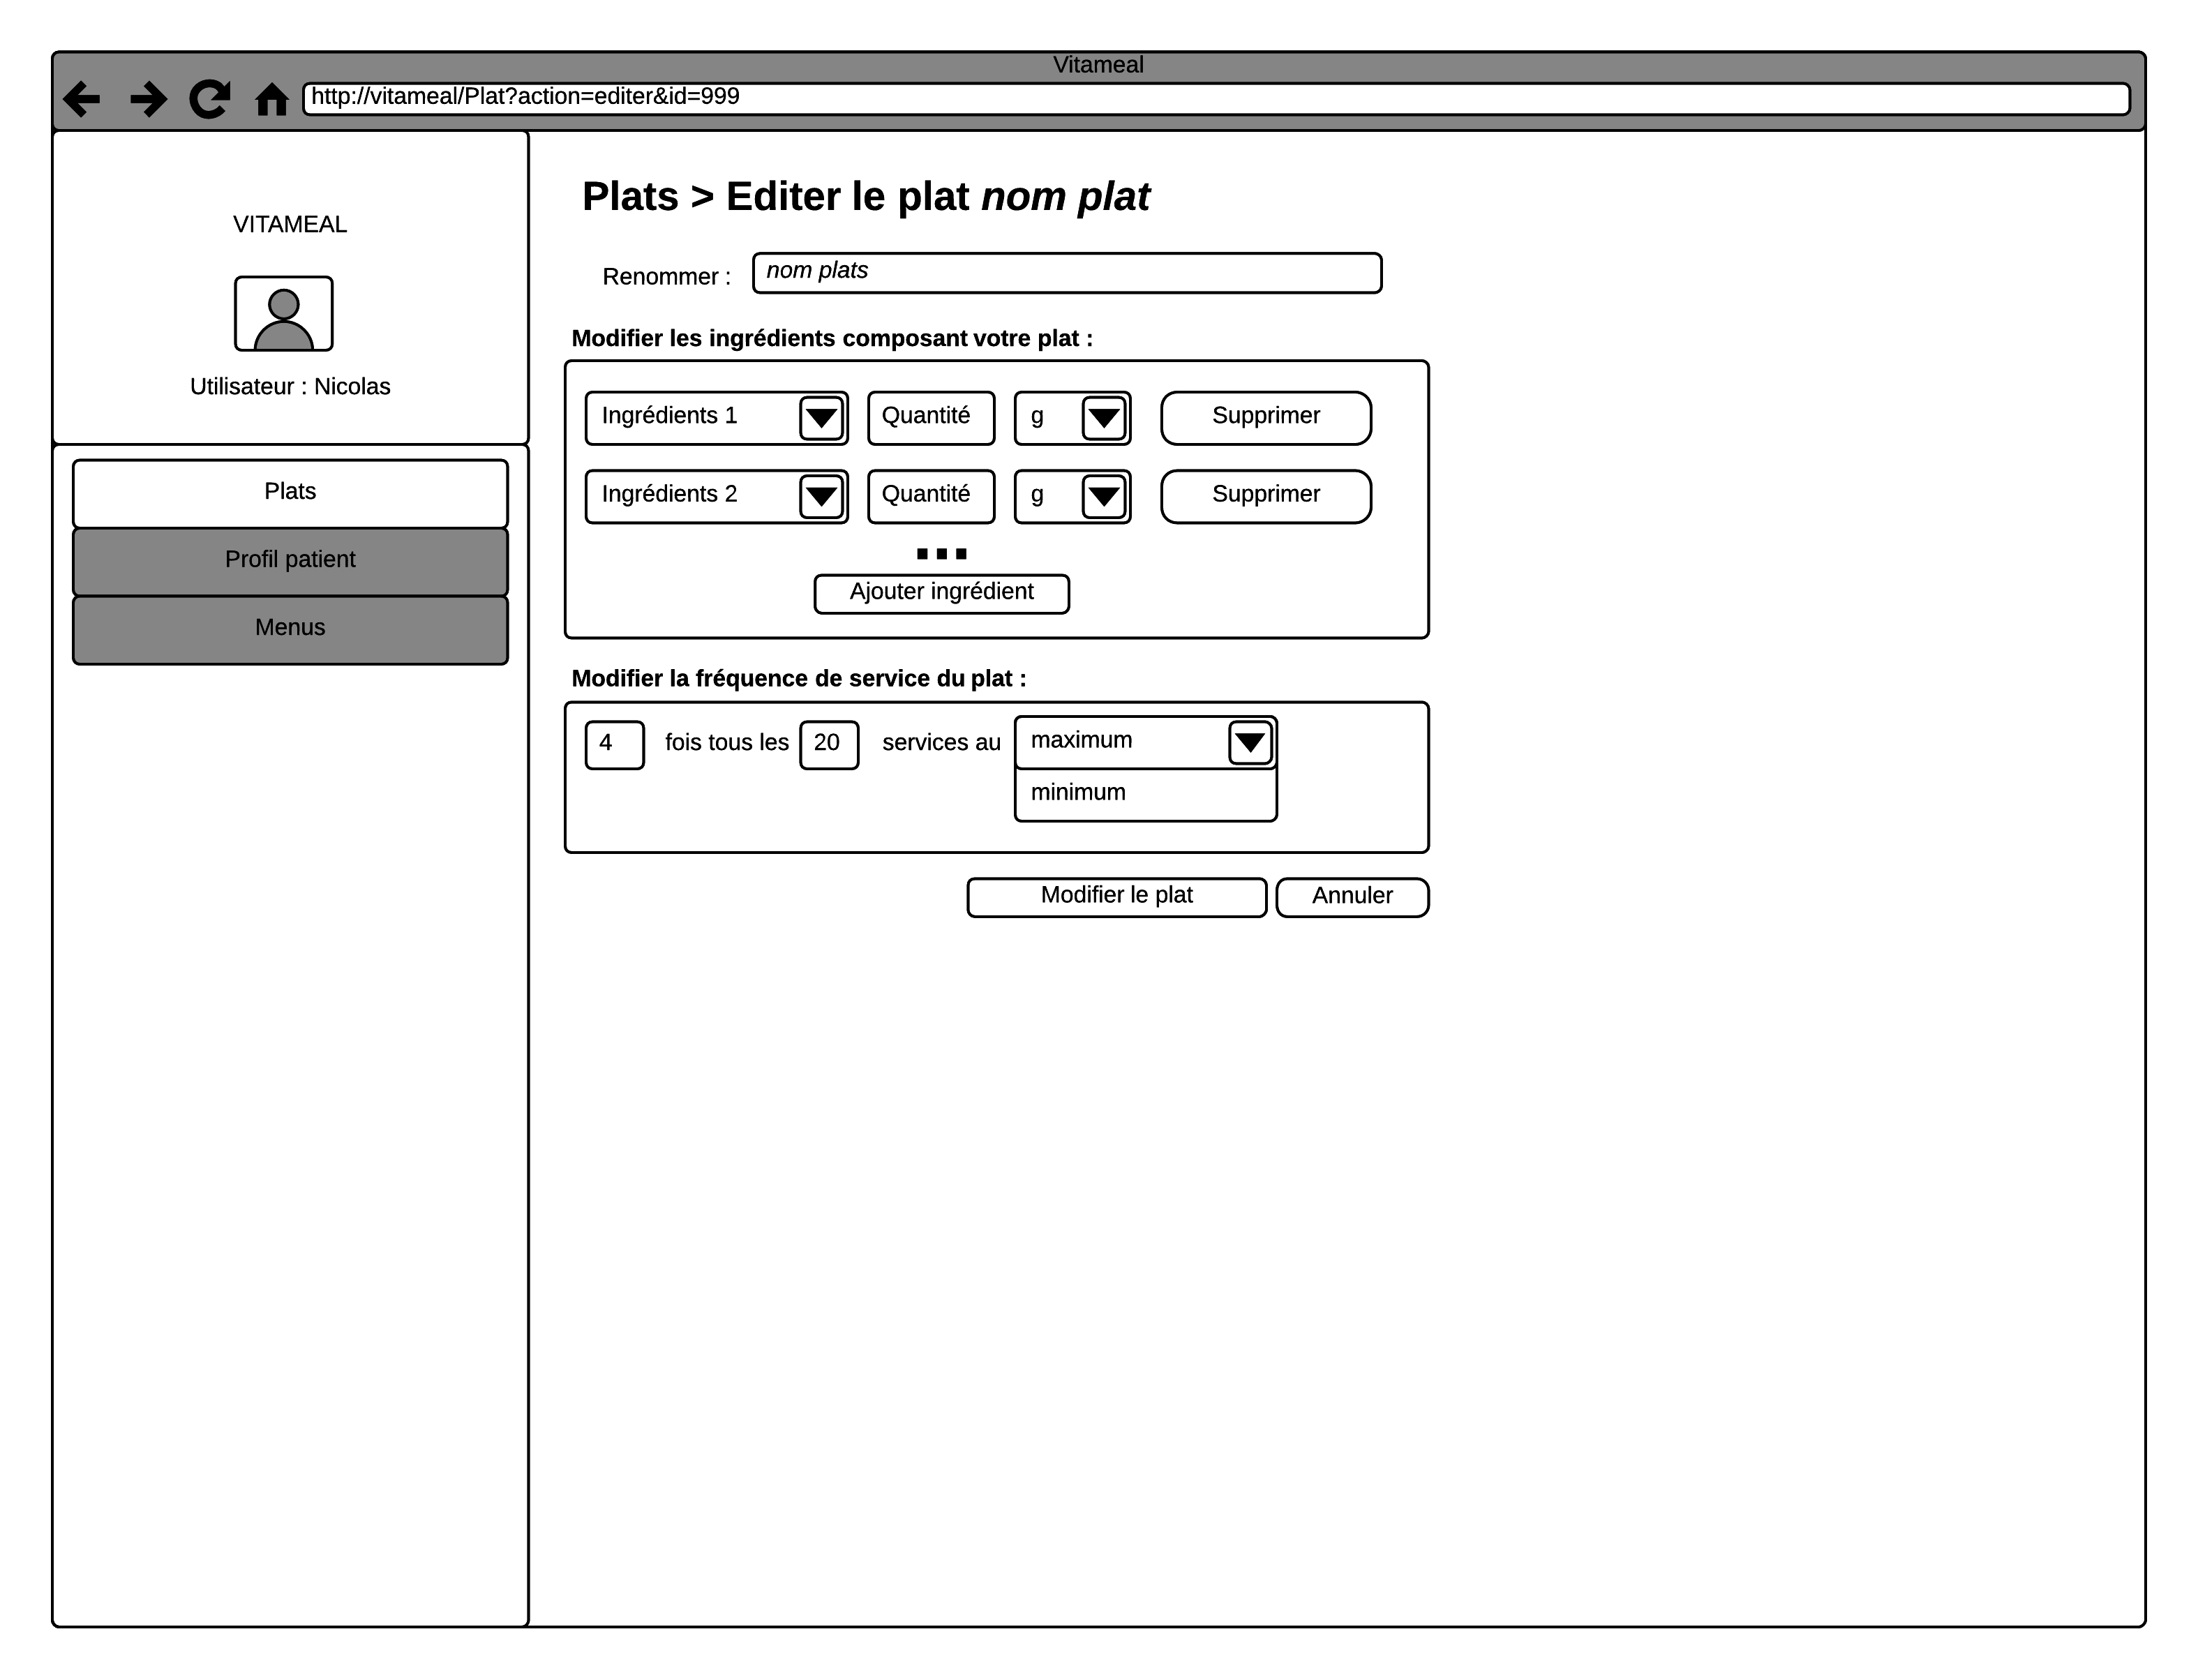
\includegraphics[scale=0.5]{../../CasDUtilisations/CompositionPlat/maquette_EcranEditionPlat.png}
\caption{Maquette de l'édition d'un plat}
\label{MaquetteEditionPlat}
\end{figure}

\begin{figure}
\centering
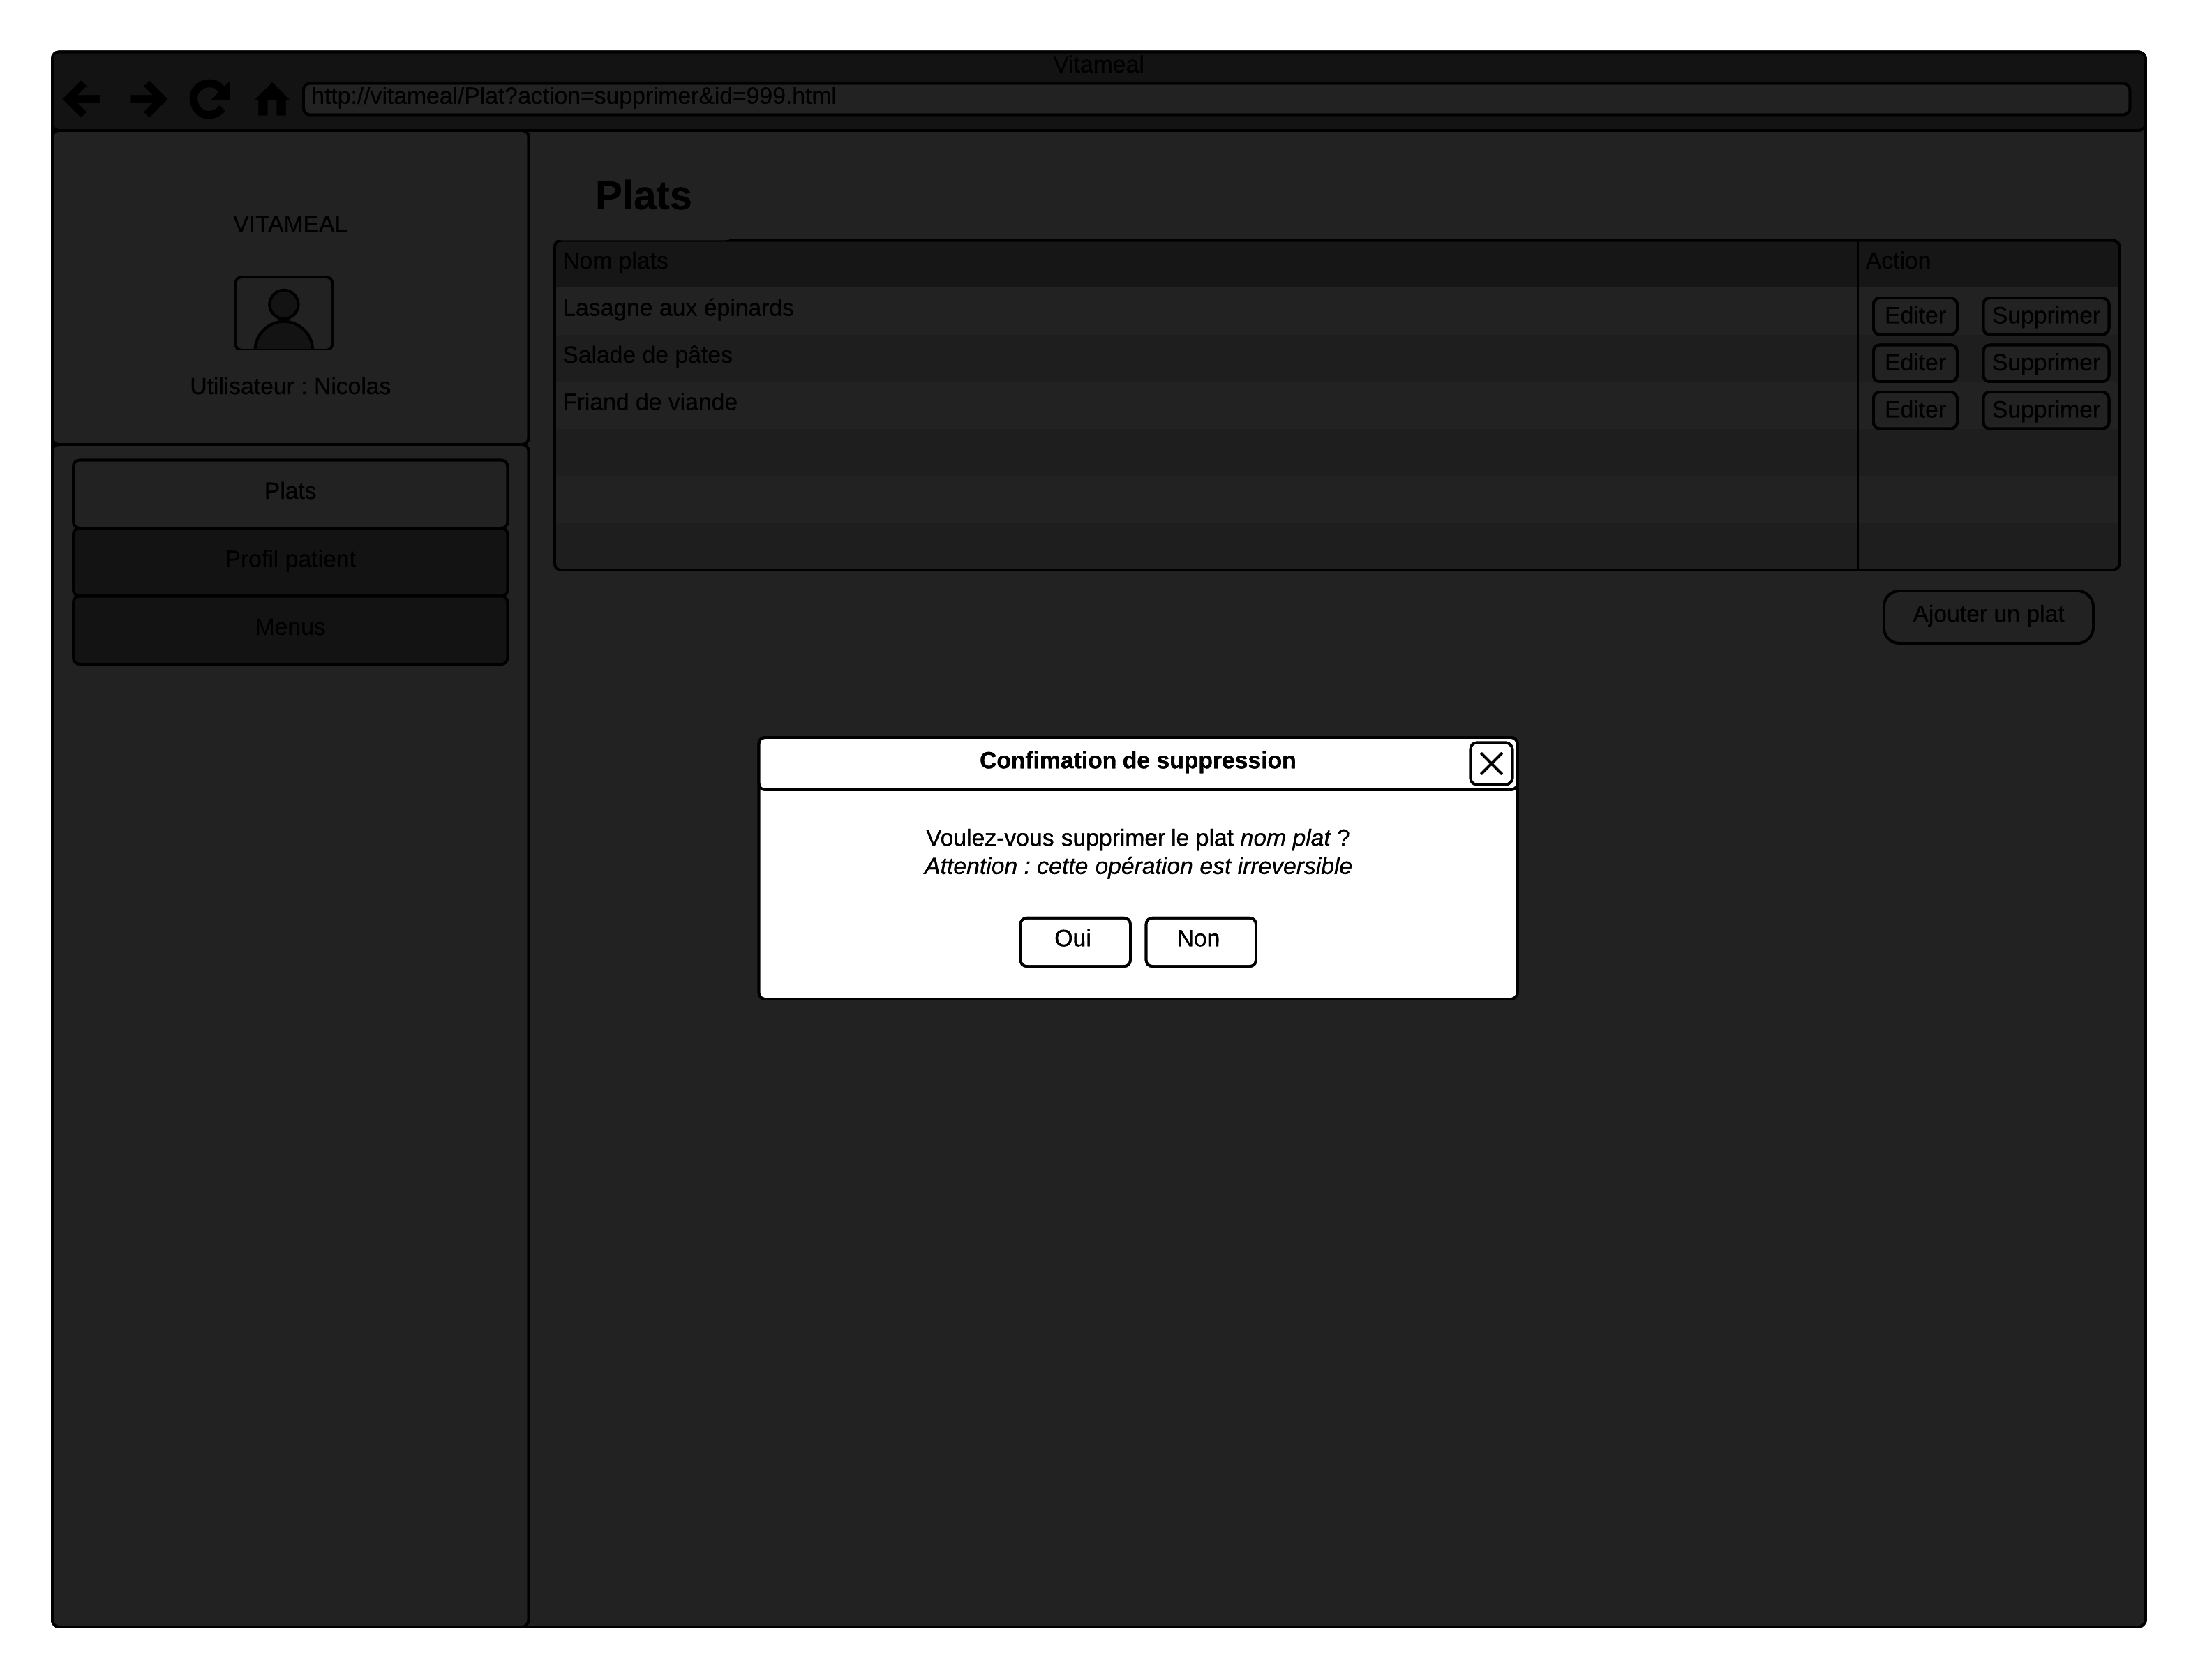
\includegraphics[scale=0.5]{../../CasDUtilisations/CompositionPlat/maquette_MessageSupressionPlat.png}
\caption{Maquette de suppression d'un plat}
\label{MaquetteSuppressionPlat}
\end{figure}


%-*- coding: utf-8 -*-
\subsubsection{Élaboration des menus}
\begin{figure}
  \centering
      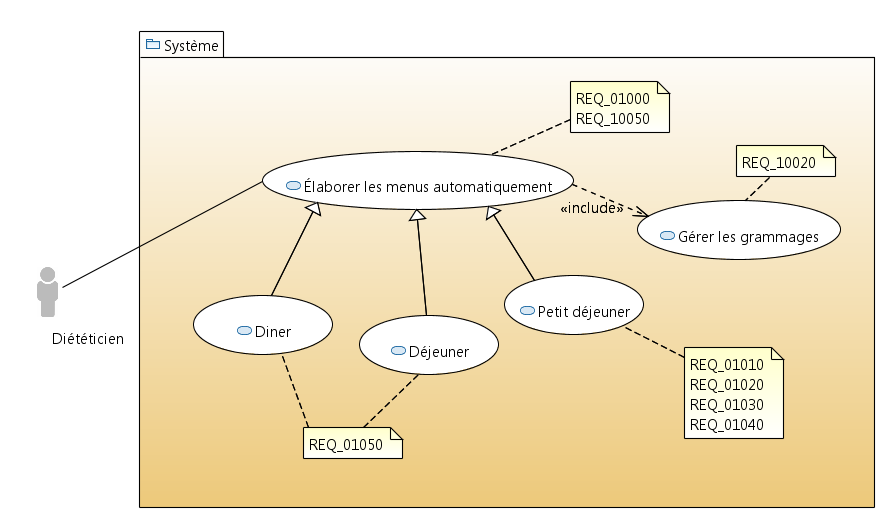
\includegraphics[width=1.00\textwidth]{../../CasDUtilisations/MenuGen/CasDUtilisation/MenuGen.png} %
\caption{Cas d'utilisation élaboration des menus}
\label{MenuGenCU}
\end{figure}

\begin{description}
\item[Nom:] Élaboration des menus (Figure \ref{MenuGenCU}).
\item[ID:] UC300
\item[Description:] Permet l'élaboration des menus.
\item[Auteur:] Jean-Félix BENITEZ.
\item[Date:] 15/06/2017
\item[Acteurs:] Diététiciens.
\item[Pré-Conditions:] Le diététicien s'est connecté au système.
\item[Scénario principal:] Figure \ref{MenuGenSeq}
  \begin{enumerate}
  \item Le diététicien sélectionne le groupe de patients pour lequel il veut générer les menus,
  \item \label{LanceElab}ensuite il lance l'élaboration des menus.
  \item L'élaboration automatique ce déroule en prenant en compte les grammages.
  \item Lorsque les menus sont élaborés, s'il estime l'élaboration correcte, il la valide.
  \item S'il estime l'élaboration incorrecte, il peut la rejeter, auquel cas il reviens à l'étape \ref{LanceElab}
  \item S'il estime l'élaboration incorrecte, il peut aussi la modifier manuellement.
  \end{enumerate}
\item[Scénario alternatif:] Aucun.
\item[Post-Conditions:] Les menus sont générés.
\end{description}

\begin{figure}
  \centering
      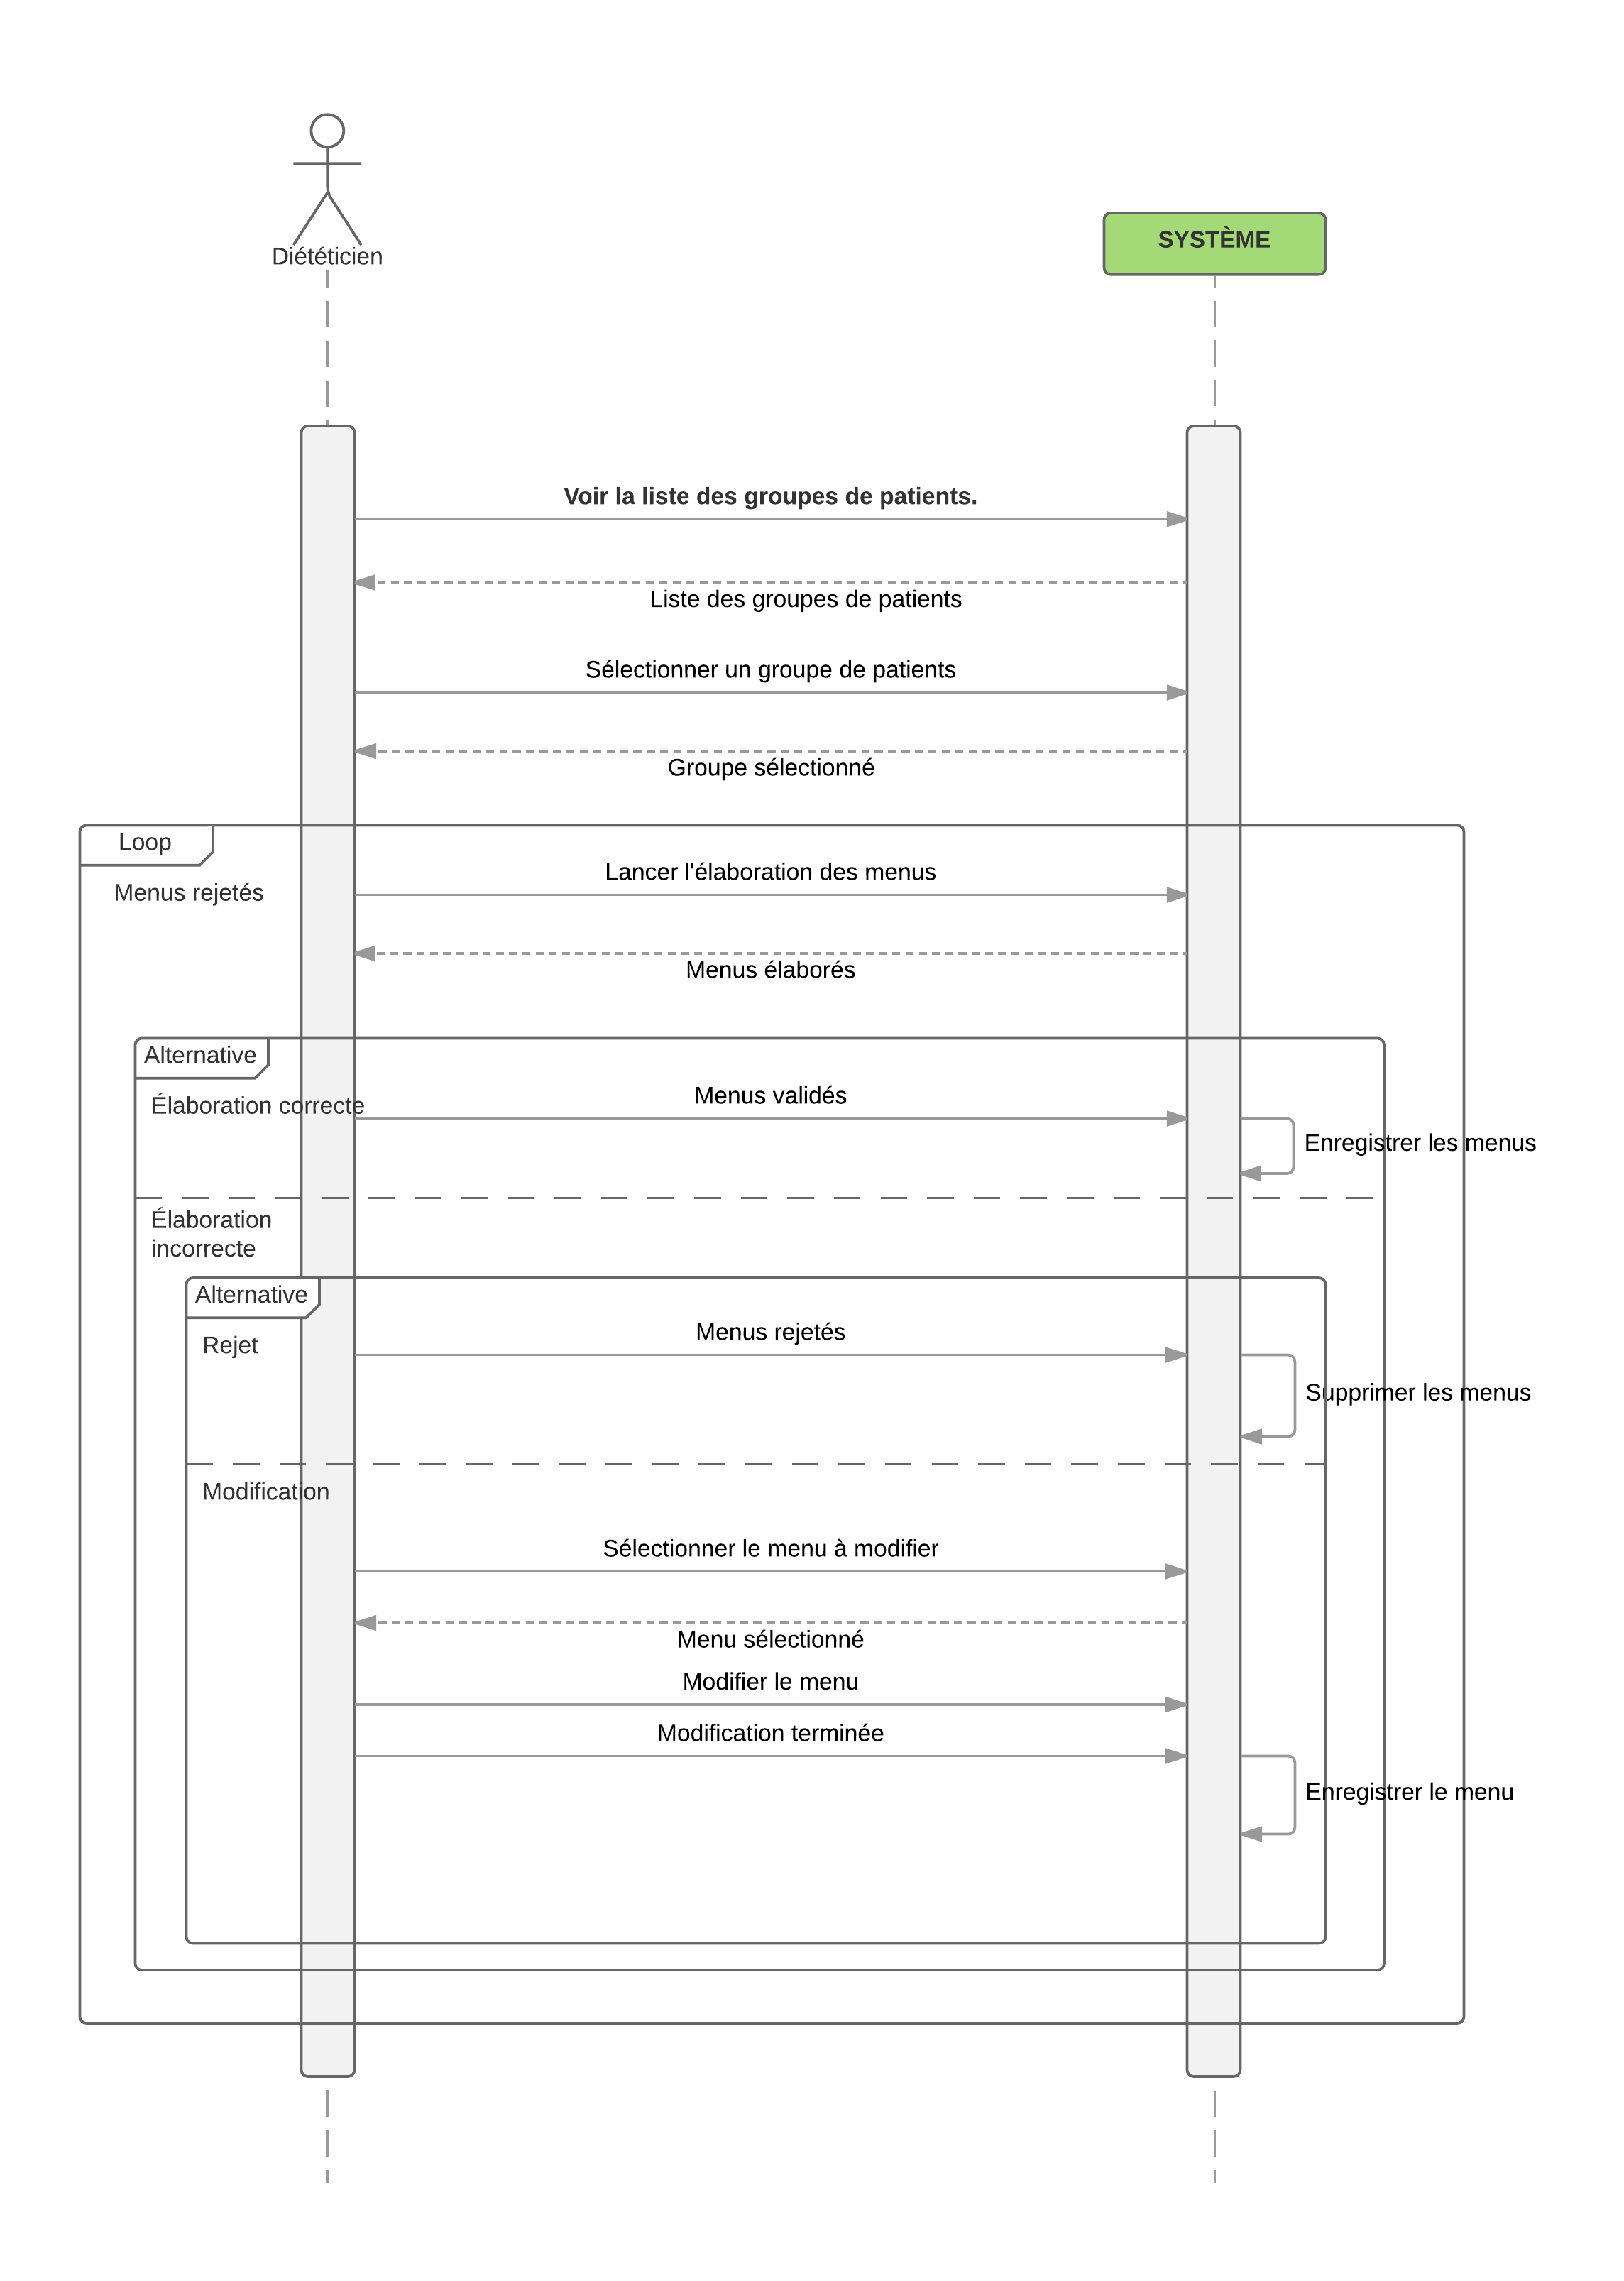
\includegraphics[width=1.00\textwidth]{../../CasDUtilisations/MenuGen/Sequence/ElaborationMenus.png} %
\caption{Séquence élaboration des menus}
\label{MenuGenSeq}
\end{figure}


%-*- coding: utf-8 -*-
\subsection{Renseigner les profils patients}

\begin{figure}[!h]
  \label{diagramme-renseigner-les-profils-patients}
  \centering
  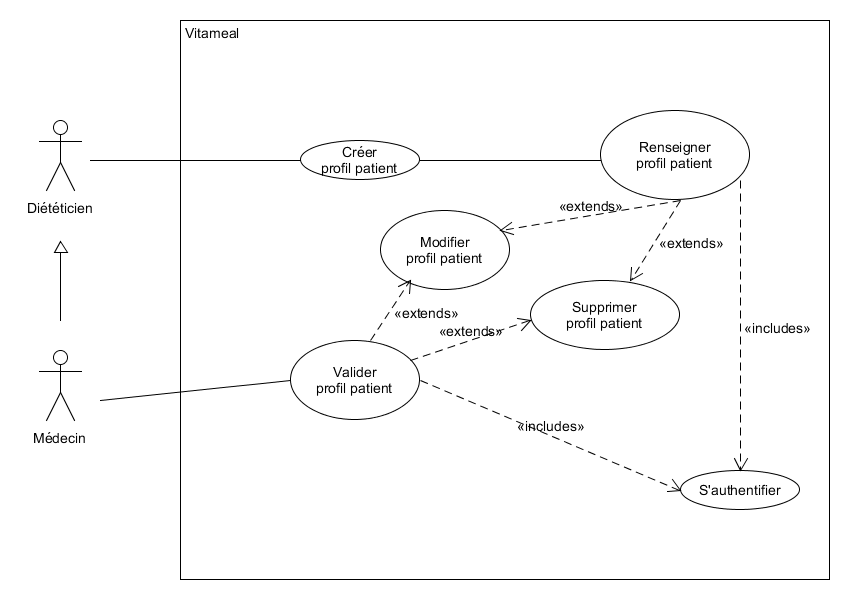
\includegraphics[width=0.9\textwidth]{../../CasDUtilisations/ProfilPatient/ProfilPatient.png}
  \caption{Use case renseigner les profils patients}
\end{figure}

\subsubsection{UC400 - Renseigner profil patient}
\begin{description}
\item [Nom :] Renseigner profil patient
\item [ID :] UC400
\item [Description :] Le diététicien souhaite pouvoir renseigner un profil patient.
\item [Auteur :] Sonia OTHMANI
\item [Date :] 08/05/2017
\item [Acteurs :] Le diététicien
\item [Pré-condition :] L’utilisateur doit être identifié en tant que diététicien (Voir cas d’utilisation \enquote{S’authentifier})
\item [Scénario principal :]
  \begin{enumerate}
  \item Le système affiche une page permettant de créer un profil patient.
  \item L’utilisateur complète les champs relatifs au patient : nom, prénom, date de naissance, pathologies, allergies, régime alimentaire prescrit.
  \item L’utilisateur valide le profil patient.
  \item Le système enregistre le profil patient.
  \end{enumerate}
\item [Scénario alternatif :] Aucun
\item [Post-Conditions :] Le profil patient est créé et enregistré.
\end{description}

\subsubsection{UC401 - Modifier profil patient}
\begin{description}
\item [Nom :] Modifier profil patient
\item [ID :] UC401
\item [Description :] Le diététicien souhaite pouvoir modifier un profil patient.
\item [Auteur :] Sonia OTHMANI
\item [Date :] 08/05/2017
\item [Acteurs :] Le diététicien
\item [Pré-condition :] L’utilisateur doit être identifié en tant que diététicien (Voir cas d’utilisation \enquote{S’authentifier})
\item [Scénario principal :]
  \begin{enumerate}
  \item Le système affiche une liste de profils patients.
  \item L’utilisateur sélectionne la fiche patient à modifier.
  \item L’utilisateur modifie le profil patient.
  \item L’utilisateur valide le profil patient.
  \item Le système enregistre le profil patient modifié.
  \end{enumerate}
\item [Scénario alternatif :] Aucun
\item [Post-Conditions :] Le profil patient est modifié et enregistré.
\end{description}

\subsubsection{UC402 - Supprimer profil patient}
\begin{description}
\item [Nom :] Supprimer profil patient
\item [ID :] UC402
\item [Description :] Le diététicien souhaite pouvoir supprimer un profil patient.
\item [Auteur :] Sonia OTHMANI
\item [Date :] 08/05/2017
\item [Acteurs :] Le diététicien
\item [Pré-condition :] L’utilisateur doit être identifié en tant que diététicien (Voir cas d’utilisation \enquote{S’authentifier})
\item [Scénario principal :]
  \begin{enumerate}
  \item Le système affiche une liste de profils patients.
  \item L’utilisateur sélectionne la fiche patient à supprimer .
  \item L’utilisateur supprime le profil patient.
  \item Le système enregistre la suppression.
  \end{enumerate}
\item [Scénario alternatif :] Aucun
\item [Post-Conditions :] Le profil patient est supprimé
\end{description}


\input{../ModeleDuDomaine/ModeleDudomaine}

%-*- coding: utf-8 -*-
\section{Backlog}
\subsection{Profil patient}
\begin{enumerate}
\item En tant que diététicien, je souhaite pouvoir créer un profil patient.
\item En tant que diététicien, je souhaite pouvoir renseigner un profil patient comportant les éléments suivants : nom, prénom, date de naissance.
\item En tant que diététicien, je souhaite pouvoir renseigner des allergies éventuelles dans le profil patient.
\item En tant que diététicien, je souhaite pouvoir renseigner un régime alimentaire prescrit, en choisissant entre les items suivants : régime sans sel, régime sans sucre, régime sans matières grasses, régime sans gluten, régime sans lactose.
\item En tant que diététicien, je souhaite pouvoir modifier un profil patient.
\item En tant que diététicien, je souhaite pouvoir supprimer un profil patient.
\item En tant que diététicien, je souhaite pouvoir gérer les patients par groupes selon leur régime prescrit, exemple le groupe des intolérants au lactose.
\item En tant que médecin, je souhaite pouvoir valider le profil diététique du patient, en plus d'effectuer toutes les actions réalisables par le diététicien.
\end{enumerate}

\subsection{Composition des plats}
\begin{enumerate}
\item En tant que diététicien, je souhaite pouvoir ajouter des plats et leurs définitions dans la listes des plats pouvant être préparés.
\item En tant que diététicien, je souhaite pouvoir descrire un plat avec sa liste d'ingrédients et les quantités nécessaires à sa réalisation.
\item Le système doit proposer un plat selon la fréquence de service de ce plat (exemple 4 fois tous les 20 repas).
  \end{enumerate}


%-*- coding: utf-8 -*-
\textcolor[RGB]{46, 116, 181}{\chapter{Architecture}}

%-*- coding: utf-8 -*-
\textcolor[RGB]{46, 116, 181}{\chapter{Codage}}

\section{Conception détaillée}

%-*- coding: utf-8 -*-
\subsubsection{Modèle du domaine}
%\rowcolors{2}{Turquoise}{} % {1}{red!26!green!29!blue!31!}{}
\begin{figure}
  \centering
      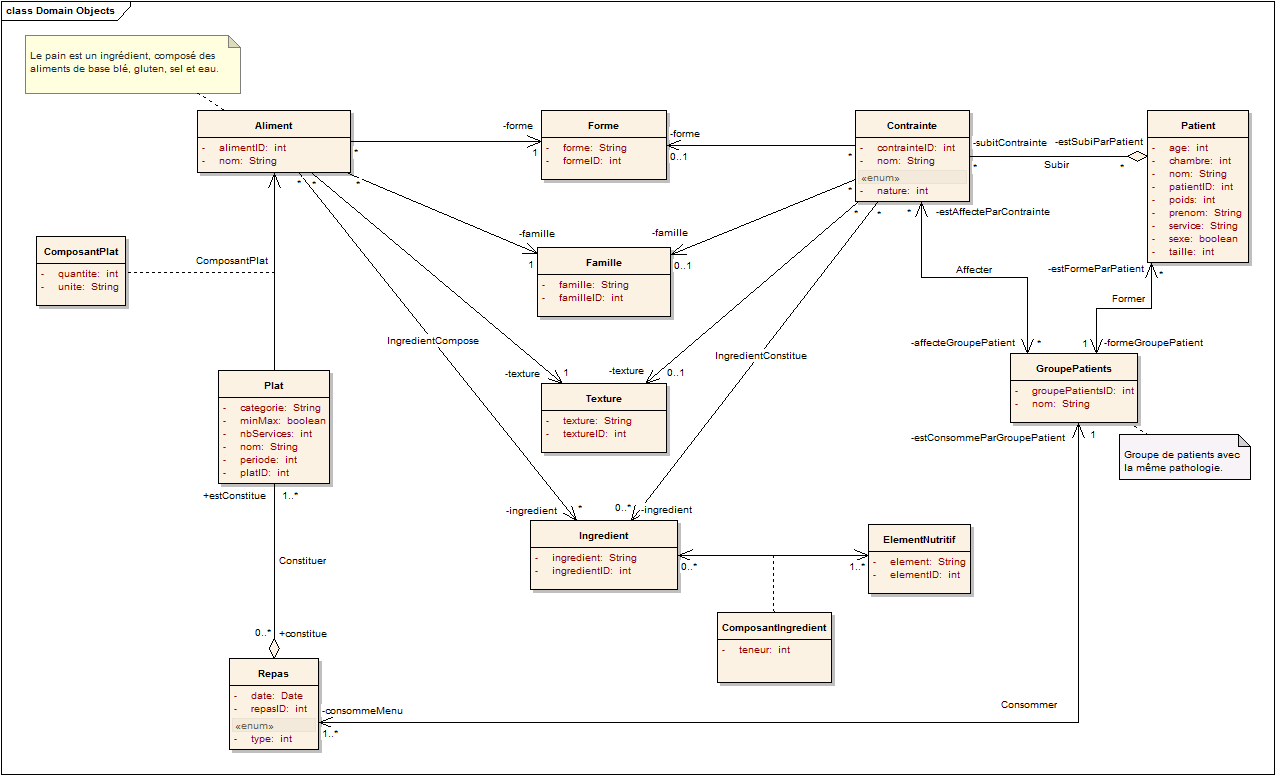
\includegraphics[angle=90, scale=0.55]{../../ModeleDuDomaine/ModeleDuDomaine.png} %
\caption{Modèle du domaine}
\label{ModeleDuDomaine}
\end{figure}

\newcommand{\classe}[1]{\emph{\textbf{#1}}}
\newcommand{\attribut}[1]{\emph{#1}}
\newcommand{\regleD}[1]{\textcolor{NavyBlue}{#1}}
\newcommand{\regleT}[1]{\textcolor{ForestGreen}{#1}}

Le modèle du domaine est représenté \autoref{ModeleDuDomaine}. Ce projet ayant pour objet l'alimentation des personnes hospitalisées, nous considérons les pathologies de ces personnes sous l'aspect de leur impact sur le plan alimentaire, et pour être plus précis sur les aliments qui s'avéreraient être interdits à cause de telle ou telle pathologie. Ces pathologies constituant des contraintes sur le plan alimentaire, c'est la classe \classe{Contrainte} qui les décrit. Elle a un attribut \attribut{nom} pour la désigner, un attribut \attribut{nature} qui permet de déterminer s'il sagit d'une allergie
\footnote{\label{allergies}\href{https://allergies.afpral.fr/allergie/en-savoir-plus-sur-les-allergies/alimentaires/89-liste-des-14-allergenes-alimentaires-majeurs}{AFPRAL: Liste des 14 allergènes alimentaires majeurs.}},
d'une contre~indications
\footnote{\label{contreIndications}La prise de certains médicaments interdit la consommation de certains aliments.}
ou d'une maladie.
Les contraintes peuvent porter aussi bien sur l'aliment luis même, que sur sa forme (solide, liquide), sa famille (fruits à coque, crustacès, ...) ou sa texture
\footnote{\label{textures}Terme métier pour dire si l'on travaille avec des \href{http://plone.vermeil.org:8080/ehpad/Bibliotheque/Memoires/annee-2012-2013/07 - Les textures modifiees et le plaisir de manger de Jacques Caby.pdf}{aliments à texture modifiée} (mixés) ou à texture maintenue (entiers).}.
Les quatres classes \classe{AlimentsBase}, \classe{Formes}, \classe{Familles} et \classe{Textures} véhicules ces informations. Elles servent aussi à renseigner la classe \classe{Ingredient} qui définit les ingrédients composant un \classe{Plat}. Les quantités misent en oeuvre sont décrites dans la classe~association \classe{ComposantPlat}. Un plat, en plus des ingrédients qui le compose, contient des informations liées à sa fréquence de service: nombre de services (\attribut{nbServices}) maximum ou minimum (\attribut{minMax}) par période (\attribut{periode}).
La classe \classe{GroupePatients} permet d'avoir la liste des patients qui subissent les mêmes contraintes alimentaires. Il y aura donc autant de menus à faire qu'il y a de groupes de patients.

\subsubsection{Modèle Logique de Données}
Le dictionnaire est décrit \autoref{DictionnaireMDD}.
\begin{description}
\item[Règle 1:] classe = relation, si héritage, les classes filles contiennent l'identifiant de la classe mère comme clè étrangère.
\regleD{\item[Règle 2:] association 1 à plusieurs devient clé étrangère de la classe fille}
\regleT{\item[Règle 3:] association plusieurs à plusieurs devient relation avec clé primaire composé des 2 clé primaires des 2 classes en relations.}
\end{description}

Ingredient(\underline{ingredientID}, nom, \regleD{famille\#}, \regleD{texture\#}, \regleD{forme\#})

\regleT{ComposantPlat(\underline{ingredientID\#, platID\#}, quantite, unite)}

Plat(\underline{platID}, nom, categorie, nbServices, periode, minMax)

\regleT{Constituer(\underline{menuID\#, platID\#})}

Menu(\underline{menuID}, date, \regleD{groupePatientsID\#})

PetitDejeuner(menuID\#)

Dejeuner(menuID\#)

Diner(menuID\#)

Patient(\underline{patientID}, prenom, nom, sexe, age, poids, taille, service, chambre, \regleD{groupePatientsID\#})

\regleT{Subir(\underline{patientID\#, contrainteID\#})}

Contrainte(\underline{contrainteID}, nom, nature, \regleD{famille\#}, \regleD{texture\#}, \regleD{forme\#})

\regleT{Affecter(\underline{groupePatientsID\#, contrainteID\#})}

GroupePatients(\underline{groupePatientsID}, nom)

Formes(\underline{forme})

Familles(\underline{famille})

Textures(\underline{texture})

AlimentsBase(\underline{alimentsBase})

\regleT{AlimentCompose(\underline{ingredientID\#, alimentsBaseID\#})}

\regleT{AlimentConstitue(\underline{contrainteID\#, alimentsBaseID\#})}
\newpage
\begin{longtable}{llp{5cm}ll}
  \hline
  \textbf{Classe} & \textbf{Attribut} & \textbf{Description} & \textbf{Type} & \textbf{Contrainte} \\ \endfirsthead \hline
  \textbf{Classe} & \textbf{Attribut} & \textbf{Description} & \textbf{Type} & \textbf{Contrainte} \\ \endhead \hline
  Ingredient & ingredientID & Clé primaire & Integer & Identifiant \\
  Ingredient & nom & Nom de l'ingredient & String & \\
  Ingredient & famille & Clé étrangère & Integer & \\
  Ingredient & texture & Clé étrangère & Integer & \\
  Ingredient & forme & Clé étrangère & Integer & \\ \hline
  ComposantPlat & ingredientID & Clé étrangère & Integer & Identifiant \\
  ComposantPlat & platID & Clé étrangère & Integer & Identifiant \\
  ComposantPlat & quantite & Quantité d'ingrédient dans le plat & Integer & \\
  ComposantPlat & unite & Unité de mesure de la quantité & String & \\ \hline
  Plat & platID & Clé primaire & Integer & Identifiant \\
  Plat & nom & Nom du plat & String & \\
  Plat & categorie & Entrée, plat ,dessert, ... & String & \\
  Plat & nbServices & Fréquence de service & Integer & \\
  Plat & periode & Période de la fréquence de service & Integer & \\
  Plat & minMax & Fréquence de service min ou max & Boolean & \\ \hline
  Constituer & menuID & Clé étrangère & Integer & Identifiant \\
  Constituer & platID & Clé étrangère & Integer & Identifiant \\ \hline
  Menu & menuID & Clé primaire & Integer & Identifiant \\
  Menu & date & Date du repas & Date &  \\
  Menu & groupePatientID &  Groupe de patients auxquels est destiné le menu & Integer & Clé étrangère \\ \hline
  PetitDejeuner & menuID & Clé étrangère & Integer & Identifiant \\ \hline
  Dejeuner & menuID & Clé étrangère & Integer & Identifiant \\ \hline
  Diner & menuID & Clé étrangère & Integer & Identifiant \\ \hline
  Patient & patientID & Clé primaire & Integer & Identifiant \\
  Patient & prenom & Prénom du patient & String & Non NULL\\
  Patient & nom & Nom du patient & String & Non NULL\\
  Patient & sexe & Sexe du patient & Boolean & \\
  Patient & age & Age du patient & Integer & $\geqslant 18$\\ %
  Patient & poids & Poids du patient & Integer & $> 0$ \\
  Patient & taille & Taille du patient & Integer & $> 0$ \\
  Patient & service & Service dans lequel ce trouve le patient & String & \\
  Patient & chambre & Numéro de chambre du patient & Integer & $> 0$ \\
  Patient & groupePatientID &  Groupe de patients auquels auquel apartient le patient & Integer & Clé étrangère \\ \hline
  Subir & patientID & Clé étrangère & Integer & Identifiant \\
  Subir & contrainteID & Clé étrangère & Integer & Identifiant \\ \hline
  Contrainte & contrainteID & Clé primaire & Integer & Identifiant \\
  Contrainte & nom & Nom de la contrainte & String & Non NULL \\
  Contrainte & nature & Nature de la contrainte & Natures & \\
  Contrainte & famille & Famille de l'ingredient & Familles & \\
  Contrainte & texture & Texture de l'ingredient & Textures & \\
  Contrainte & forme & Forme de l'ingredient & Formes & \\ \hline
  Affecter & groupePatientsID & Clé étrangère & Integer & Identifiant \\
  Affecter & contrainteID & Clé étrangère & Integer & Identifiant \\ \hline
  GroupePatients & groupePatientsID & Clé primaire & Integer & Identifiant \\
  GroupePatients & nom & Nom du groupe de patients & String & \\ \hline
  Formes & forme & Clé primaire & Integer & Identifiant \\ \hline
  Familles & famille & Clé primaire & Integer & Identifiant \\ \hline
  Textures & texture & Clé primaire & Integer & Identifiant \\ \hline
  AlimentsBase & alimentBase & Clé primaire & String &  \\ \hline
  AlimentCompose & alimentBase & Clé étrangère & String &  \\
  AlimentCompose & ingredientID & Clé étrangère & Integer & Identifiant \\ \hline
  AlimentConstitue & alimentBase & Clé étrangère & String &  \\
  AlimentConstitue & contrainteID & Clé étrangère & Integer & Identifiant \\ \hline
\caption{Dictionnaire}
\label{DictionnaireMDD}
\end{longtable}

%\hiderowcolors


%-*- coding: utf-8 -*-
\subsection{Préparer menus}


%-*- coding: utf-8 -*-
\subsection{Consulter menus}


%-*- coding: utf-8 -*-
\subsection{Composer plat}


%-*- coding: utf-8 -*-
\subsubsection{Élaboration des menus}
\begin{figure}
  \centering
      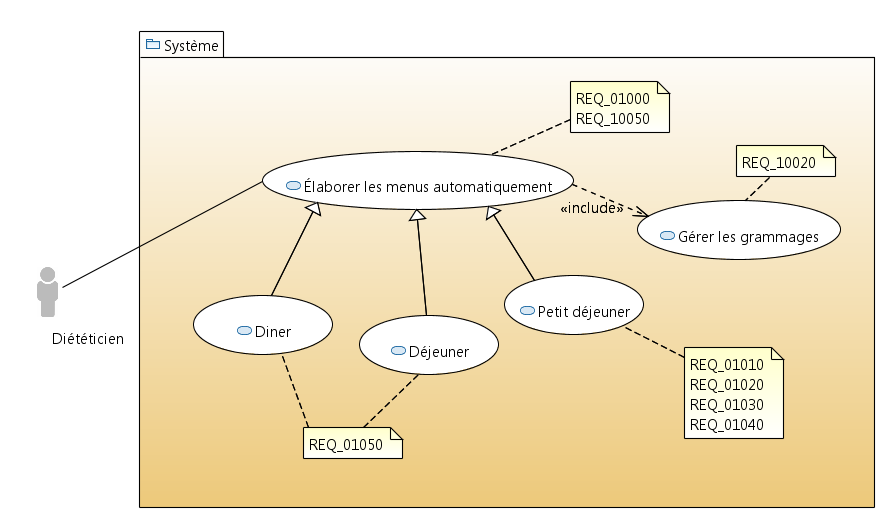
\includegraphics[width=1.00\textwidth]{../../CasDUtilisations/MenuGen/CasDUtilisation/MenuGen.png} %
\caption{Cas d'utilisation élaboration des menus}
\label{MenuGenCU}
\end{figure}

\begin{description}
\item[Nom:] Élaboration des menus (Figure \ref{MenuGenCU}).
\item[ID:] UC300
\item[Description:] Permet l'élaboration des menus.
\item[Auteur:] Jean-Félix BENITEZ.
\item[Date:] 15/06/2017
\item[Acteurs:] Diététiciens.
\item[Pré-Conditions:] Le diététicien s'est connecté au système.
\item[Scénario principal:] Figure \ref{MenuGenSeq}
  \begin{enumerate}
  \item Le diététicien sélectionne le groupe de patients pour lequel il veut générer les menus,
  \item \label{LanceElab}ensuite il lance l'élaboration des menus.
  \item L'élaboration automatique ce déroule en prenant en compte les grammages.
  \item Lorsque les menus sont élaborés, s'il estime l'élaboration correcte, il la valide.
  \item S'il estime l'élaboration incorrecte, il peut la rejeter, auquel cas il reviens à l'étape \ref{LanceElab}
  \item S'il estime l'élaboration incorrecte, il peut aussi la modifier manuellement.
  \end{enumerate}
\item[Scénario alternatif:] Aucun.
\item[Post-Conditions:] Les menus sont générés.
\end{description}

\begin{figure}
  \centering
      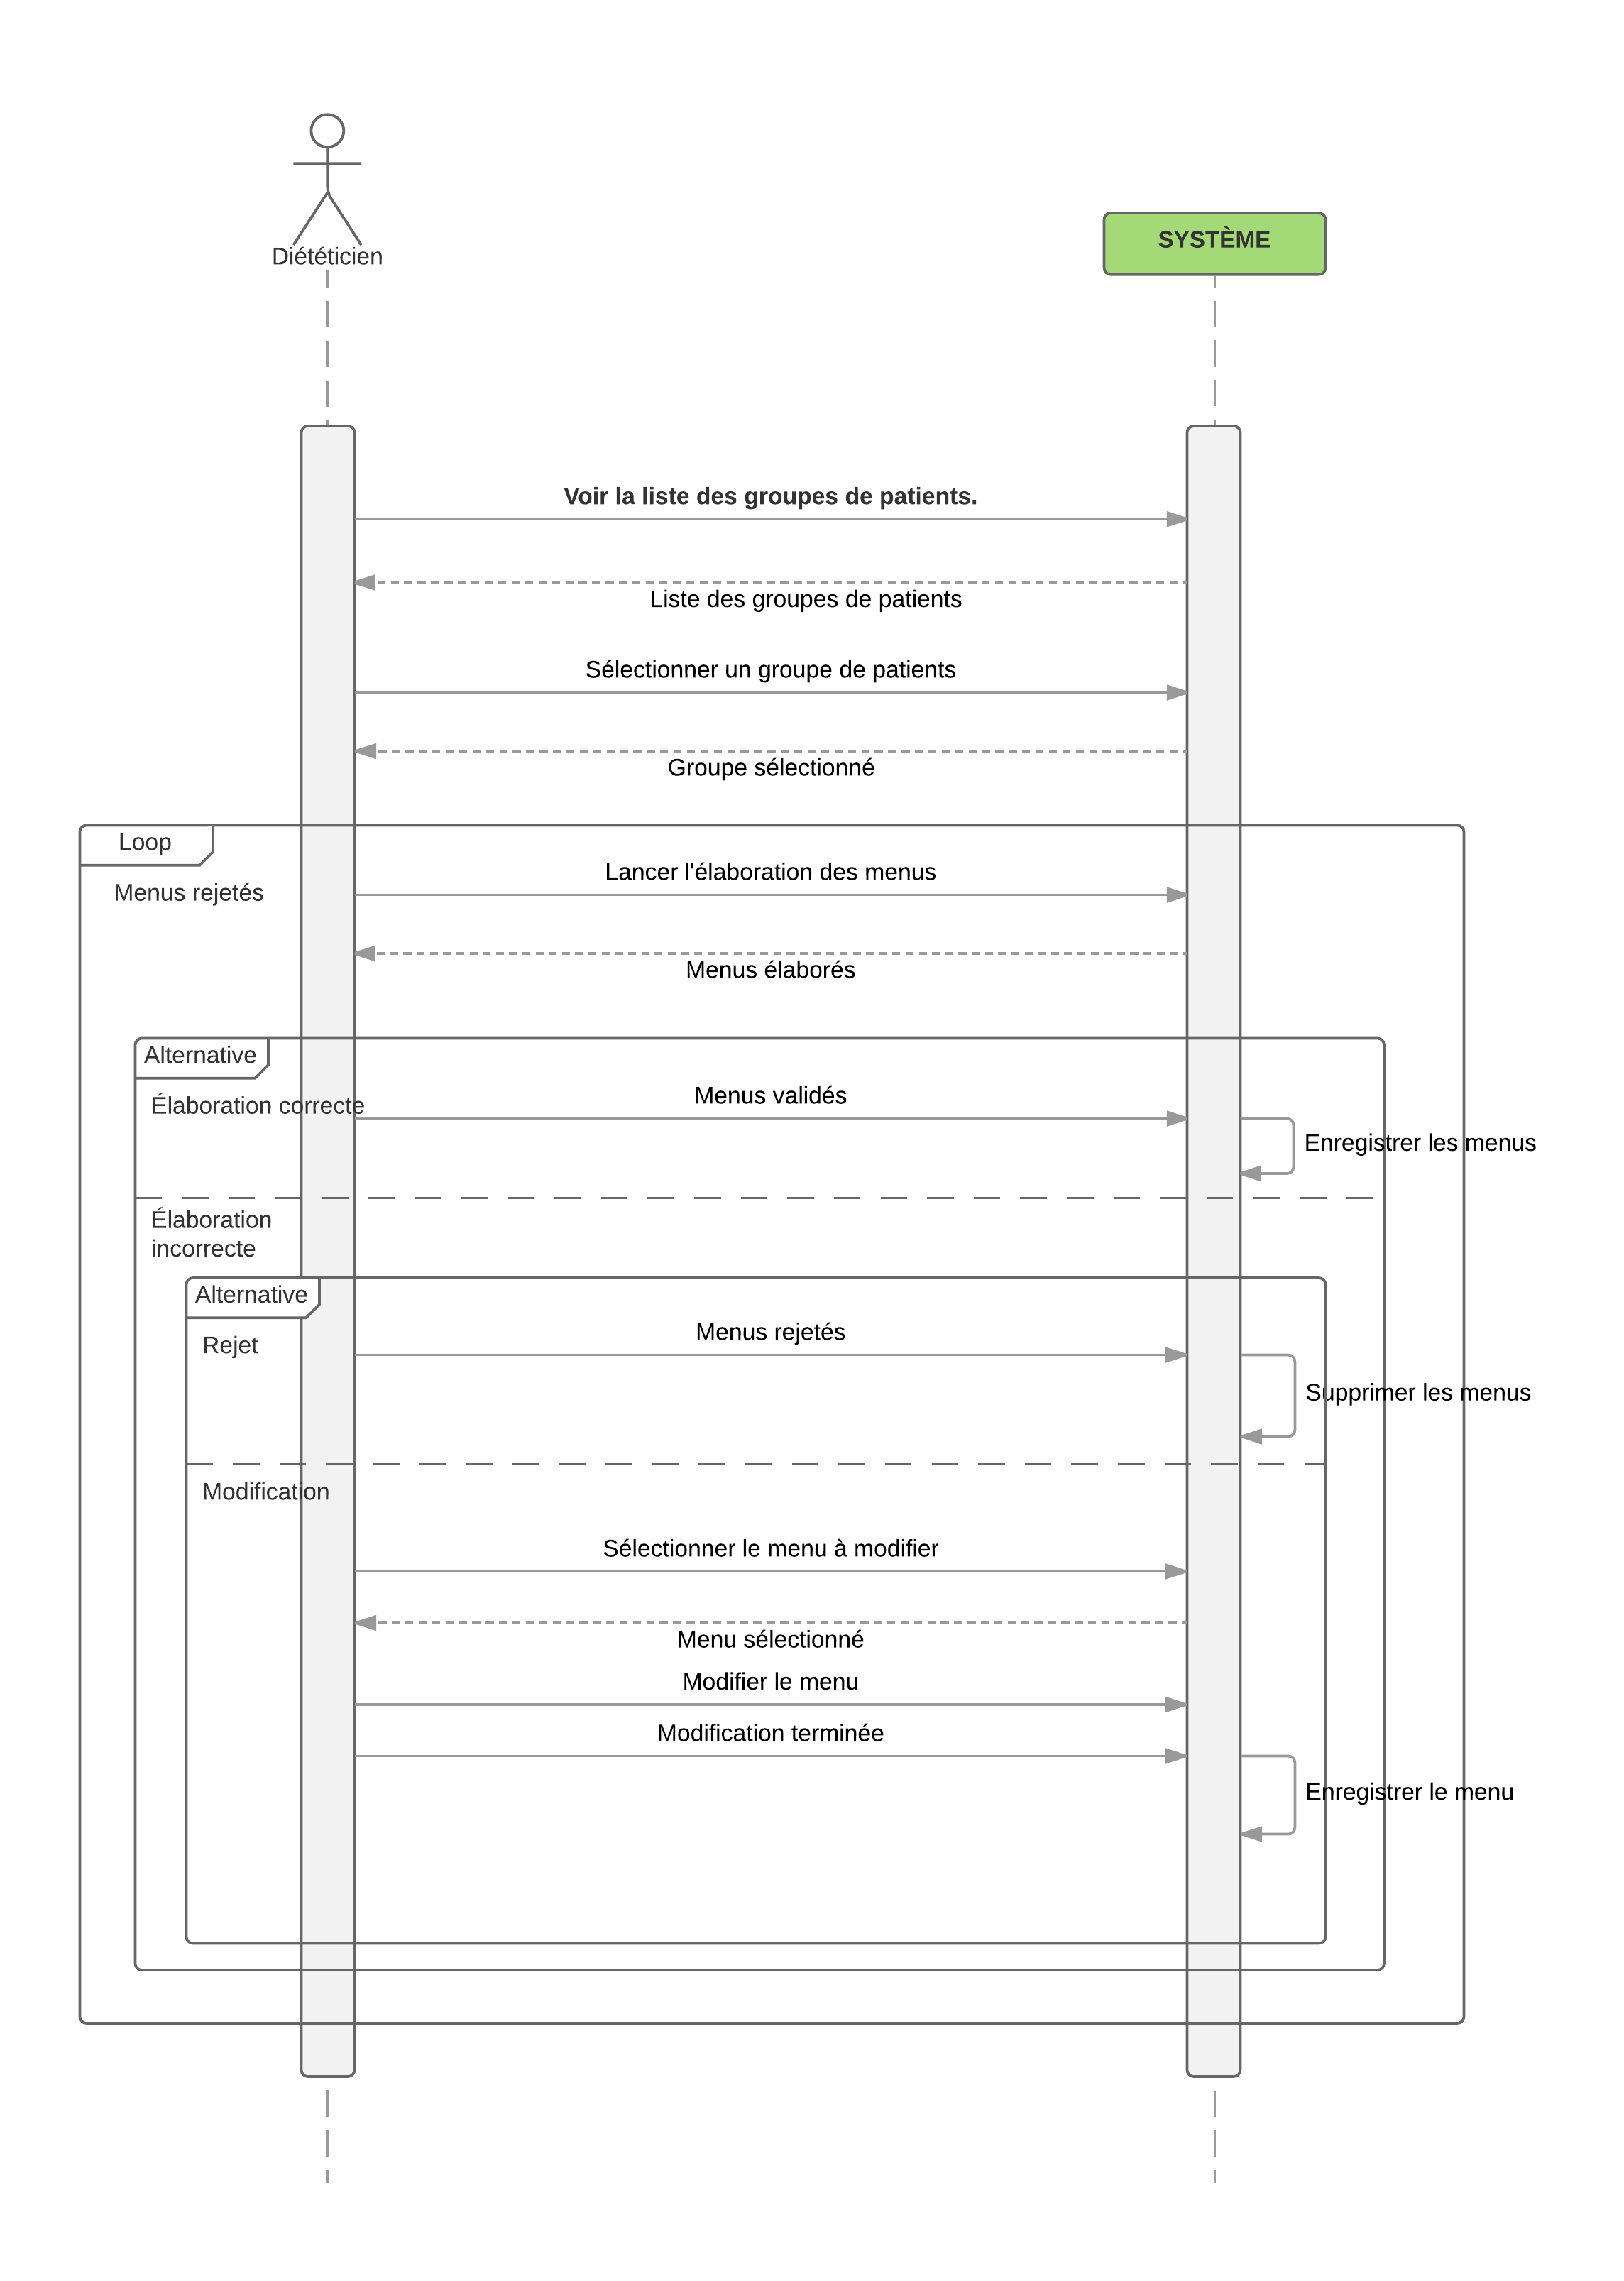
\includegraphics[width=1.00\textwidth]{../../CasDUtilisations/MenuGen/Sequence/ElaborationMenus.png} %
\caption{Séquence élaboration des menus}
\label{MenuGenSeq}
\end{figure}


%-*- coding: utf-8 -*-
\subsection{Renseigner profil patient}

L'analyse du cas d'utilisation renseigner un profil pâtient se fait en plusieurs opérations : l'ajout, la modification, suppression et la validation de profil patient, qui sont implémentées selon un modèle MVC.

\begin{figure}
  \label{diagramme-renseigner-les-profils-patients}
  \centering
  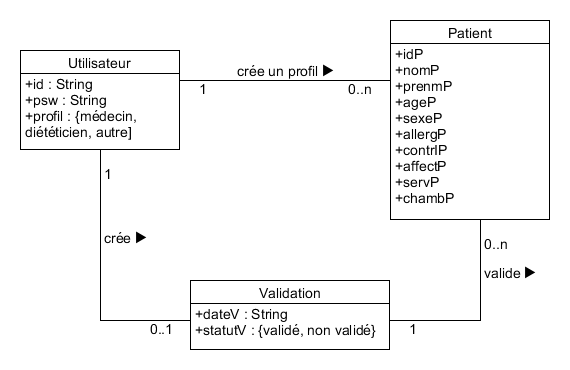
\includegraphics[width=0.9\textwidth]{../../CasDUtilisations/ProfilPatient/diagclassProfilPatient.png}
  \caption{Diagramme de classe renseigner les profils patients}
\end{figure}


\begin{figure}
  \label{diagramme-renseigner-les-profils-patients}
  \centering
  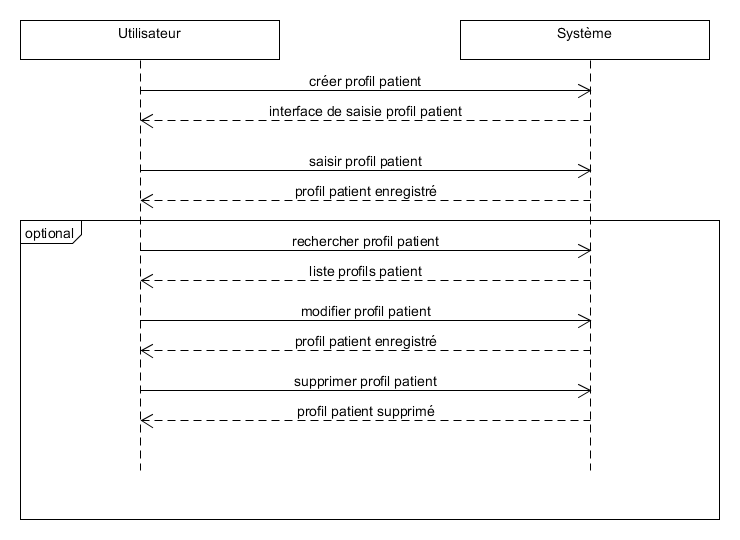
\includegraphics[width=0.9\textwidth]{../../CasDUtilisations/ProfilPatient/diagseqProfilPatient.png}
  \caption{Diagramme de séquence renseigner les profils patients}
\end{figure}

\begin{figure}
  \label{diagramme-renseigner-les-profils-patients}
  \centering
  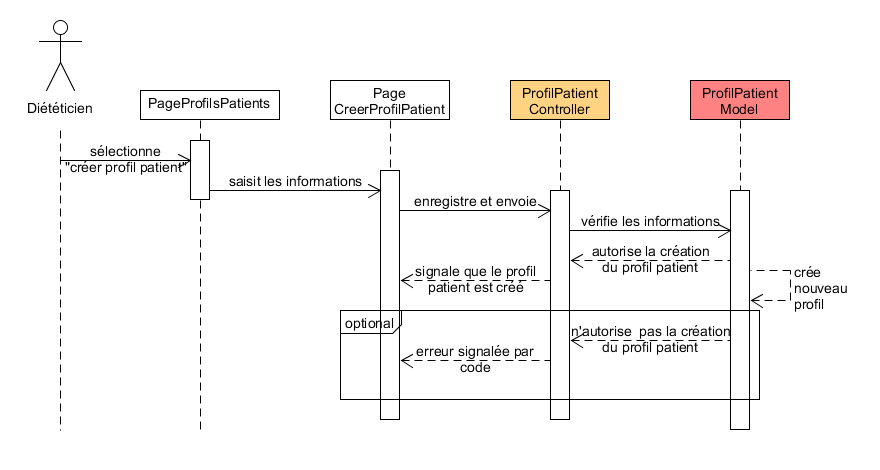
\includegraphics[width=0.9\textwidth]{../../CasDUtilisations/ProfilPatient/diagSrqDetaillProfilPatient.png}
  \caption{Diagramme de séquence détaillé renseigner les profils patients}
\end{figure}

\begin{figure}
  \label{diagramme-renseigner-les-profils-patients}
  \centering
  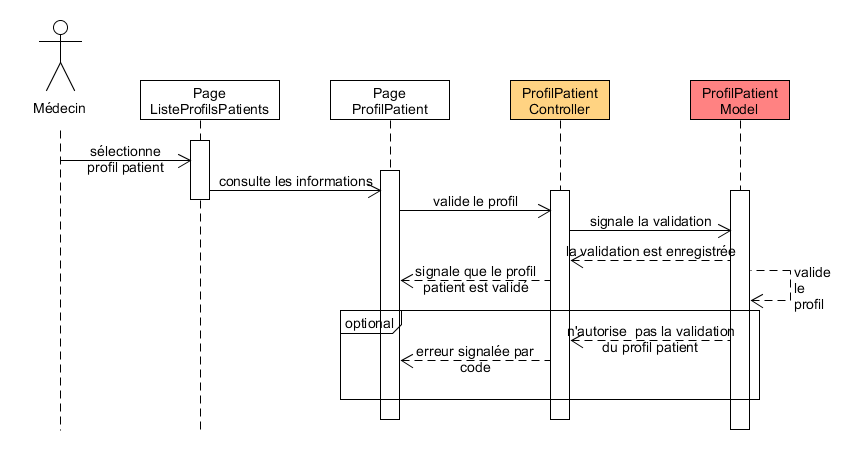
\includegraphics[width=0.9\textwidth]{../../CasDUtilisations/ProfilPatient/diagSrqDetaillValidProfilPatient.png}
  \caption{Diagramme de séquence détaillé valider les profils patients}
\end{figure}


\section{Intégration}
\colorbox{yellow}{TODO}

\section{Tests}
\colorbox{yellow}{TODO}

%-*- coding: utf-8 -*-
\textcolor[RGB]{46, 116, 181}{\chapter{Bilan}}


\appendix
\newcommand{\annexe}[1]{%
	\refstepcounter{chapter}%
	\phantomsection%
	\addcontentsline{toc}{chapter}{\appendixname~{\thechapter}: #1}%
	\chapter*{\appendixname~{\thechapter}: #1}}
\chapter{Composition des repas}

\label{annexeA}

\section{Le petit-déjeuner}

\subsection{Composition}

Le petit-déjeuner comporte au minimum les éléments suivants :
\begin{itemize}
	\item une boisson : eau, jus de fruit (100\% fruit, sans sucre ajoutée), lait demi écrémé, café, café décaféinée, thé, tisane, chicorée, ... ;
	\item un aliment céréalier : pain, biscottes, ou autre produit céréalier, ... ;
	\item un produit laitier : lait, yaourt, fromage ou autre produit laitier, ... ;
	\item un fruit : fruit cru, jus de fruit, compote, purée de fruit.
\end{itemize}

Le lait est considéré comme une boisson et un produit laitier et le jus de fruit est considéré comme une boisson et comme un fruit.

Selon type de population, le petit-déjeuner peut éventuellement être complété par :
\begin{itemize}
	\item un élément lipidique  : beurre, margarine, ... ;
	\item un élément sucré : confiture, gelée, miel, ... ;
	\item un élément protidique : jambon, oeuf, ... .
\end{itemize}

\subsection{Restrictions}

Il convient d'éviter les pâtes à tartiner et les pâtisseries contenant plus de 15 \% de matières grasses, c'est à dire :

les viennoiseries (croissant, pain au chocolat, ...), les barres chocolatées, les biscuits chocolatés ou fourrés, les céréales fourrées, les beignets, les gaufres, les crêpes fourrées au chocolat, les gâteaux à la crème ou au chocolat, les brownies au chocolat et aux noix, les quatre-quarts, les gâteaux moelleux chocolatés type napolitain mini-roulé, les biscuits chocolatés, les biscuits sablés nappés de chocolat, les biscuits secs chocolatés, les galettes ou les sablés, les goûters chocolatés fourrés, les gaufrettes fourrées, les madeleines, les biscuits secs feuilletés type palmier, les cookies au chocolat.

Ainsi que les desserts suivant :

les tiramisus,les crèmes brûlées, les glaces ou les nougats glacés.

La fréquence recommandée est de 3 repas sur 20 repas successifs au maximum.

\subsection{Références}

\ref{docNutrition}, § 3.2.1 (page 17), § 4.2.1.1.4 (page 39)

\section{Le déjeuner et le souper}

\subsection{Composition}

Le déjeuner et le souper se composent de quatre ou cinq composantes selon le tableau ci-dessous. Cinq composantes donnent plus de latitude et de souplesse dans la mise en œuvre des fréquence de services (\colorbox{yellow}{TODO}).

\newcommand\Chbx{\centering{\CheckedBox}}

\begin{center}

\begin{tabular}{|l|c|c|c|c|}
	\hline
	\textbf{Composantes} & \textbf{5 composantes} & \multicolumn{3}{|c|}{\textbf{4 composantes}} \\
	\hline
	Entrée & \checkmark & \checkmark & \checkmark ** & \cellcolor{gray} \\
	\hline
	Plats protidiques & \checkmark & \checkmark & \checkmark & \checkmark \\
	\hline
	Garnitures & \checkmark & \checkmark & \checkmark & \checkmark \\
	\hline
	Produits laitiers & \checkmark & \cellcolor{gray} & \checkmark & \checkmark \\
	\hline
	Desserts & \checkmark & \checkmark ** & \checkmark & \checkmark \\
	\hline
	Pain & \multicolumn{4}{|c|}{Présence systématique} \\
	\hline
	Eau & \multicolumn{4}{|c|}{Présence systématique} \\
	\hline
\end{tabular}

\end{center}

\noindent * Seule boisson indispensable, du lait demi-écrémé non sucré peut aussi être proposé. \\
** Présence obligatoire d'un produit laitier dans l'entrée ou le dessert.

\vspace{0.5cm}

Les composantes des repas principaux sont généralement constituées de : 
\begin{itemize}
	\item Les entrées : crudités, cuidités, entrées de légumes secs et ou d’autres féculents, entrées protidiques (oeuf, poisson), préparations pâtissières salées, charcuteries ;
	\item Les plats protidiques : plat principal à base de viande, poisson, oeuf, abats. Préparations pâtissières salées servies en plat principal (crêpes salées, friands divers, pizzas, tartes, quiches, tourtes). Charcuteries servies en plat principal (préparation traditionnelle à base de chair de porc, boudin noir, saucisses diverses, crépinettes, ...) ;
	\item Les garnitures : légumes, légumes secs, pommes de terre, produits céréaliers ;
	\item Les produits laitiers : Lait demi-écrémé, lait fermenté ou autre produit laitier frais, fromage, dessert lacté ;
	\item Les desserts : fruit crus entier ou en salade, fruit cuit ou au sirop, pâtisserie, biscuit, sorbet, dessert lacté, glace.
\end{itemize}

\subsection{Restrictions}

Il est déconseillé de distribuer des boissons sucrées.

\subsection{Références}

\ref{docNutrition}, § 3.2.3 (page 18-19)
\label{LastPage}
\end{document}
